%%%%%%%%%%%%%%%%%%%%%%%%%%%%%%%%%%%%%%%%%%%%%%%%%%%%%%%%%%%%%%%%
%                                                               %
%             sPHENIX BUP for 2020           %
%                                                               %
%%%%%%%%%%%%%%%%%%%%%%%%%%%%%%%%%%%%%%%%%%%%%%%%%%%%%%%%%%%%%%%%%

\documentclass[11pt,twoside,notitlepage]{book}

\RequirePackage{lineno}
\usepackage{import}
\usepackage{titlesec}
\usepackage{enumitem}
\usepackage{amssymb, amsmath}
\usepackage{mathpazo}
\usepackage{float,graphicx}
\graphicspath{{figs/}} 
\usepackage[figuresright]{rotating}
\usepackage[usenames,dvipsnames]{color}
\usepackage{microtype}
\usepackage{tabulary}
\usepackage{booktabs,multirow,dcolumn,bigdelim}
\newcommand{\otoprule}{\midrule[\heavyrulewidth]}
\usepackage{xr-hyper}
\usepackage[pdftex,plainpages=false,pdfpagelabels,backref,pdfborder={0 0 0}]{hyperref}
\usepackage{url}
\usepackage[toc,page,titletoc]{appendix}
\usepackage{afterpage}
\usepackage[font=small,labelfont=bf]{caption}
\setlength\captionmargin{15pt}
\usepackage[scaled]{helvet}
\usepackage{sectsty}
\allsectionsfont{\normalfont\sffamily}
\usepackage{titletoc}
\titlecontents{chapter}
  [1.5em]
  {\linespread{0.9}\normalfont\sffamily\bfseries}
  {\contentslabel{2em}} 
  {\hspace*{-2.3em}} 
  {\mdseries\titlerule*[1pc]{.}\contentspage} 
\titlecontents{section}
  [3.5em]
  {\linespread{0.9}\normalfont\sffamily}
  {\contentslabel{2.3em}} 
  {\hspace*{-2.3em}} 
  {\titlerule*[1pc]{.}\contentspage} 
\titlecontents{subsection}
  [4.5em]
  {\linespread{0.9}\normalfont\sffamily}
  {\contentslabel{2.3em}} 
  {\hspace*{-2.3em}} 
  {\titlerule*[1pc]{.}\contentspage} 
\titlecontents{subsubsection}
  [5.5em]
  {\linespread{0.9}\normalfont\sffamily}
  {\contentslabel{2.3em}} 
  {\hspace*{-2.3em}} 
  {\titlerule*[1pc]{.}\contentspage} 
\tolerance = 10000

\usepackage[text={6.5in,8.75in},headheight=15pt,centering]{geometry}
\usepackage{xspace}
\usepackage{siunitx}
\DeclareGraphicsExtensions{.pdf,.png,.jpg}
\DeclareUnicodeCharacter{2009}{\,}

\newcommand{\filenamedot}{.}
\setlength{\parindent}{0.0in}
\setlength{\parskip}{0.1in}
\renewcommand{\topfraction} {0.9}
\renewcommand{\bottomfraction} {0.9}
\renewcommand{\textfraction} {0.1}
\renewcommand{\floatpagefraction} {0.8}

\renewcommand{\arraystretch}{1.9}
%\addtolength{\tabcolsep}{-0.5pt}

\usepackage{fancyhdr}
\pagestyle{fancy}
\renewcommand{\chaptermark}[1]{\markboth{#1}{}}
\renewcommand{\sectionmark}[1]{\markright{#1}{}}
\fancyhead{} % clear all header fields 
\fancyhead[RO,LE]{\sffamily \rightmark}
\fancyhead[LO,RE]{\sffamily \leftmark}
\fancyfoot{} % clear all footer fields 
\fancyfoot[RO,LE]{\sffamily \thepage}
\renewcommand{\headrulewidth}{0pt} 
\fancypagestyle{plain}{%
  \fancyhf{}
  \fancyfoot[RO,LE]{\sffamily \thepage}
}

\usepackage{eurosym}
\usepackage{xcolor}
\usepackage{framed}
\colorlet{shadecolor}{blue!10}

\setcounter{secnumdepth}{2}
\setcounter{tocdepth}{1}

\newcommand{\hic}{\mbox{$A$$+$$A$}\xspace}
\newcommand{\pA}{\mbox{$p$$+$$A$}\xspace}
\newcommand{\AuAu}{\mbox{Au$+$Au}\xspace}
\newcommand{\auau}{\mbox{Au$+$Au}\xspace} 
\newcommand{\alal}{\mbox{Al$+$Al}\xspace} 
\newcommand{\oo}{\mbox{O$+$O}\xspace} 
\newcommand{\agag}{\mbox{Ag$+$Ag}\xspace} 
\newcommand{\cucu}{\mbox{Cu$+$Cu}\xspace} 
\newcommand{\raa}{\mbox{$R_{AA}$}\xspace}
\newcommand{\pbpb}{\mbox{Pb$+$Pb}\xspace} \newcommand
{\pdau}{\mbox{$p(d)$$+$Au}\xspace} \newcommand
{\aj}{\mbox{$A_J$}\xspace} \newcommand {\pp}{\mbox{$p$$+$$p$}\xspace}
\newcommand {\ppbar}{\mbox{$p$$+$$\overline{p}$}\xspace}
\newcommand{\pT}{\mbox{${p_T}$}\xspace}
\newcommand{\jpsi}{\mbox{$J/\psi$}}
\newcommand{\sqrtsnn}{\mbox{$\sqrt{s_{\scriptscriptstyle NN}}$}}
\newcommand{\npart}{$N_\mathrm{part}$}
\newcommand{\ncoll}{$N_\mathrm{coll}$}
\newcommand{\qgp}{\mbox{quark-gluon plasma}\xspace}
\newcommand{\jt}{\mbox{$J_T$}} \newcommand{\qhat}{\mbox{$\hat{q}$}}
\newcommand{\Qsqr}{\mbox{$Q^2$}} \newcommand{\CuCu}{\mbox{Cu$+$Cu}}
\newcommand{\PbPb}{\mbox{Pb$+$Pb}} \newcommand{\pPb}{\mbox{$p$$+$Pb}}
\newcommand{\gjet}{\mbox{$\gamma$-jet}}
\newcommand{\Qmax}{\mbox{$Q_{\max}$}} \newcommand{\ET}{\mbox{$E_T$}}
\newcommand{\Et}{\mbox{$E_T$}} \newcommand{\kt}{\mbox{$k_T$}}
\newcommand{\RAA}{\mbox{$R_{AA}$}\xspace} \newcommand{\IAA}{\mbox{$I_{AA}$}}
\newcommand{\pt}{\mbox{${p_T}$}\xspace}
\newcommand{\highpt}{high-${\rm p_{_{T}}}$}
\newcommand{\lessim}{{\stackrel{<}{\sim}}} \newcommand{\eqnpt}{p_T}
\newcommand{\eA}{\mbox{$e-{\rm A}$}}
\newcommand{\dAu}{\mbox{$d$$+$Au}\xspace}
\newcommand{\pAu}{\mbox{$p$$+$Au}\xspace}
\newcommand{\pau}{\mbox{$p$$+$Au}\xspace}
\newcommand{\GeVSQ}{\mbox{${\rm GeV}^2$}}
\newcommand{\fastjet}{\mbox{\sc FastJet}\xspace}
\newcommand{\geant}{\mbox{\sc Geant4}\xspace}
\newcommand{\antikt}{\mbox{anti-$k_T$}\xspace}
\newcommand{\pythia}{\mbox{\sc Pythia}\xspace}
\newcommand{\rapgap}{\mbox{\sc Rapgap}\xspace}
\newcommand{\milou}{\mbox{\sc Milou}\xspace}
\newcommand{\pyquen}{\mbox{\sc Pyquen}\xspace}
\newcommand{\hijing}{\mbox{\sc Hijing}\xspace}
\newcommand{\roofit}{\mbox{\sc RooFit}\xspace}
\newcommand{\roounfold}{\mbox{\sc RooUnfold}\xspace}
\newcommand{\beetle}{\mbox{\sc Beetle}\xspace}
\newcommand{\gj}{\mbox{$\gamma$+jet}\xspace}
\newcommand{\gh}{\mbox{$\gamma$+hadron}\xspace}
\newcommand{\martinimusic}{\mbox{\sc Martini+Music}\xspace}
\newcommand{\martini}{\mbox{\sc Martini}\xspace}
\newcommand{\music}{\mbox{\sc Music}\xspace}
\newcommand{\Ephenix}{Electron-Ion Collider (EIC) detector built
  around the BaBar magnet and sPHENIX calorimetry\xspace}
\newcommand{\ephenix}{EIC detector built around the BaBar magnet and
  sPHENIX calorimetry\xspace} 
\newcommand{\refdesign}{reference design\xspace}
\newcommand{\refconfig}{reference configuration\xspace}
\newcommand{\dijet}{\mbox{dijet}\xspace}
\newcommand{\fake}{\mbox{fake}\xspace}
\newcommand{\fast}{\mbox{fast}\xspace}
\newcommand{\veryfast}{\mbox{very fast}\xspace}
\newcommand{\epem}{\mbox{$e^+e^-$}\xspace}
\newcommand{\onewidth}{0.6\linewidth}
\newcommand{\twowidth}{0.48\linewidth}
\newcommand{\threewidth}{0.32\linewidth}

\newcommand{\egoing}{\mbox{electron-going}\xspace}
\newcommand{\hgoing}{\mbox{hadron-going}\xspace}
\newcommand{\egodir}{electron-going direction\xspace}
\newcommand{\hgodir}{hadron-going direction\xspace}


\newcommand{\lyxdot}{.}
\usepackage{subfig}

\setlength\fboxsep{0pt}
\setlength\fboxrule{0.5pt}

\begin{document} 

\linenumbers

\frontmatter

\pagestyle{empty}
\newpagecolor{black}\afterpage{\restorepagecolor}
\renewcommand*\familydefault{\sfdefault}
{\sffamily

\vspace*{\fill}
\noindent
\makebox[0pt][l]{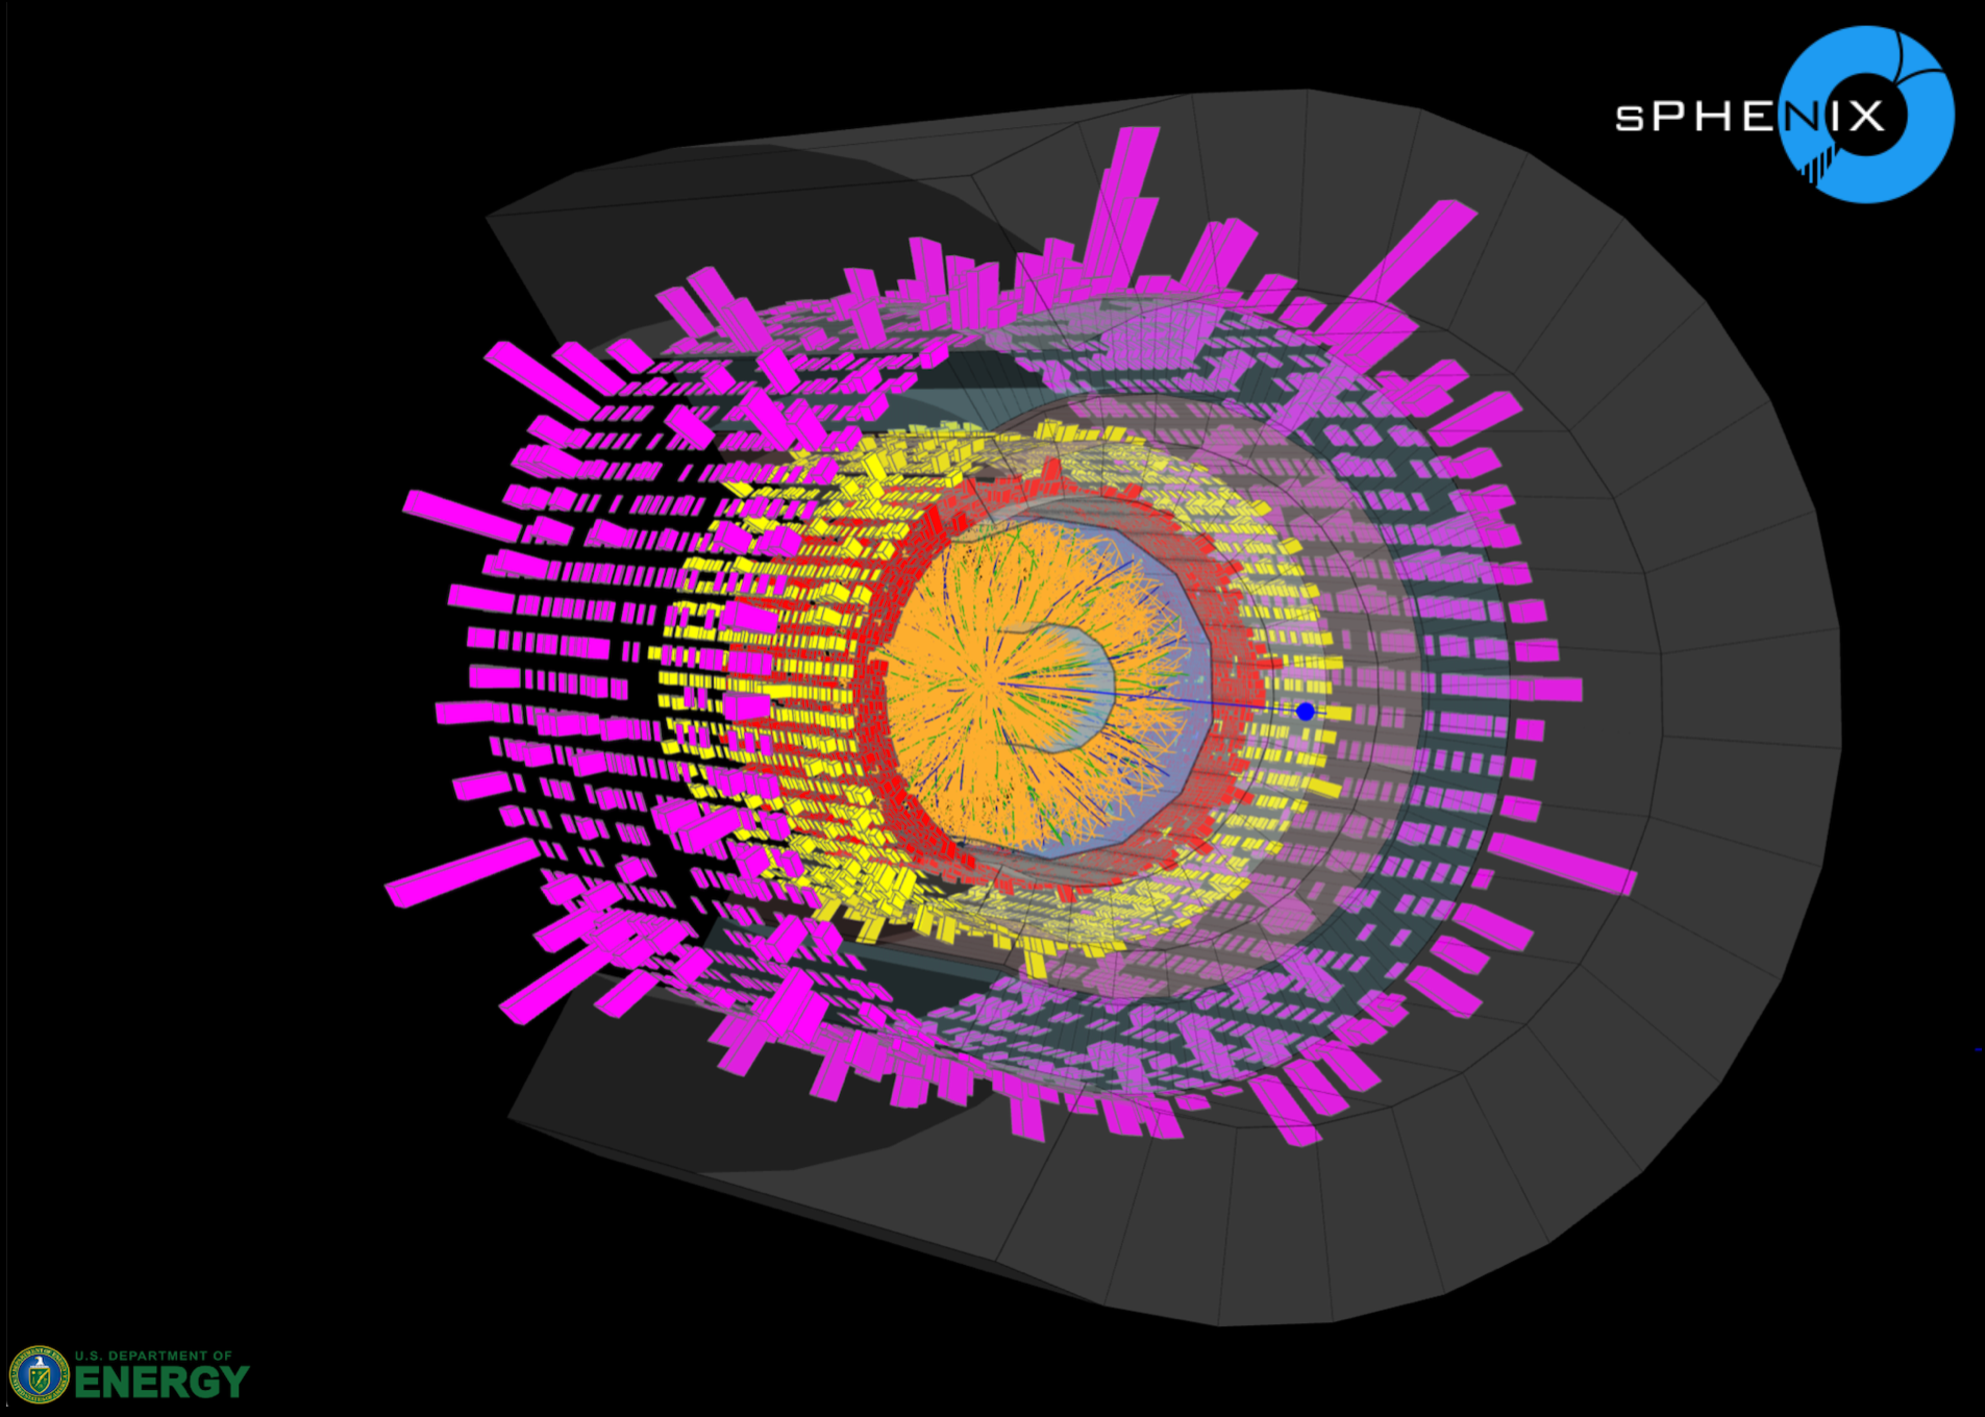
\includegraphics[width=\linewidth]{figs/EventDisplayAuAuLogo.pdf}}
\vspace*{\fill}

\begin{center}
  \begin{tabular}{c}
    \emph{\Large{\textcolor{white}{sPHENIX Beam Use Proposal}}} \\
    \large{\textcolor{white}{September 10, 2020}}
  \end{tabular}
\end{center}
}

\renewcommand*\familydefault{\rmdefault}


\cleardoublepage
\pagestyle{fancy}
\chapter*{Executive Summary}
\label{executive_summary}
\setcounter{page}{1}

sPHENIX will be the first new collider detector at RHIC in over twenty
years, focusing measurement capabilities on heavy-ion collisions in
this energy range that have not been available before.  The experiment
is a specific priority of the DOE/NSF NSAC Long Range Plan, and the
significance of its expected results, complementing those coming from
the LHC, was highlighted in the WG5 Heavy-Ion input to the European
Strategy for Particle Physics.  sPHENIX will play a critical role in
the completion of the RHIC science mission by enabling qualitatively
new measurements of the microscopic nature of quark-gluon plasma.
These studies rely on very high statistics measurements of jet
production, jet substructure and open and hidden heavy flavor over an
unprecedented kinematic range at RHIC.  They are enabled by the high
rate capability and large acceptance of the detector, combined with
high precision tracking and electromagnetic and hadronic calorimetry.

The effort to construct the experiment is officially underway, with
the DOE MIE project having been granted PD-2/3 approval in September
2019.  Additional detectors, funded as BNL capital projects (such as
the MVTX micro-vertex tracker) or realized as contributions from
collaborating institutions, are also under construction and will be
integrated into the full experiment, completing its science
capabilities.  The sPHENIX resource-loaded schedule leads to a first
year of operation in 2023; the final year of sPHENIX operations in
2025 is dictated by BNL's reference schedule for the EIC project.
This document responds to a charge (see Appendix~\ref{chap:charge})
from the BNL NPP ALD to detail the sPHENIX run plan during the years
2023--2025.

In the run plan described in this document, each of the three years
plays a critical role in fulfilling the science mission outlined in
the NP Long Range Plan:
\begin{itemize}
\item Year-1 serves to commission all detector subsystems and full
  detector operations, and to validate the calibration and
  reconstruction operations essential to delivering the sPHENIX
  science in a timely manner. Close coordination with C-AD will be
  required in the ramp-up of RHIC luminosity and optimization of beam
  operations to achieve these goals in a safe manner, enabling full
  exploitation of RHIC luminosity in Year-2 and Year-3. Year-1 will
  also allow collection of a \auau data set enabling sPHENIX to repeat
  and extend measurements of ``standard candles at RHIC.
\item Year-2 will see commissioning of the detector for \pp collisions
  (unless extended running beyond 24 cryo-weeks and successful \auau
  commissioning permits doing this already in Year-1) and collection
  of a large p+p reference data set, as well as a large \pAu data set
  for studies of cold QCD.
\item Year-3 is focused on collection of a very large statistics \auau
  data set for measurements of jets and heavy flavor observables with
  unprecedented statistical precision and accuracy.
\end{itemize}

We also outline a plan for additional running, should the occasion
arise. This represents unique opportunities for collecting massive,
archival \auau and spin polarized \pp data sets in the final years of
RHIC operation.

Table~\ref{tab:exec:summary1} provides an overview of the data we
expect to obtain in Year-1 to Year-3, as requested in the ALD charge,
and Table~\ref{tab:exec:summary2} summarizes possibilities for
additional run periods.

%We describe a plan with three main features:
%\begin{itemize}
%\item A three year run plan that delivers the physics of the sPHENIX science proposal.
%\item A first year that prioritizes proper commissioning of the
%  sPHENIX detector.  Close coordination with C-AD will be required to
%  validate beam handling strategies that will enable full exploitation
%  of RHIC luminosity in years two and three of the plan.
%\item A plan for additional running, should the occasion arise, that
%  represents a unique opportunity for a massive, archival \auau and
%  spin polarized \pp data set in the final years of RHIC operation.
%\end{itemize}
%
%The priority in the first year of sPHENIX operation will be to
%properly commission and calibrate the detector.  Assuming this goes
%well, we would then plan to take several weeks of \auau data.  The
%priority oef the second year is to record the data for the \pp
%baseline.  In a 24 cryo-week scenario, it would be difficult to go
%beyond this plan.  In a sufficiently long run, we would switch species
%and record \pAu data as well.  The third year of running focues on a
%large statistics \auau run.  With the \pp baseline and the \auau data,
%we would be able to carry out the goals of the sPHENIX science
%proposal.  Table~\ref{tab:exec:summary1} summarizes the data we would
%expect to obtain. 

\begin{table}[hbt!]
\centering
\caption{\label{tab:exec:summary1} Summary of sPHENIX Beam Use Proposal for the years
  2023--2025, as requested in the charge.  Details are provided in
  Chaper~\ref{chap:beam_use_proposal}.} 
\bigskip \centering \begin{tabular}{ | c | c | c | c | c | c | c | }
\hline
Year & Species & $\sqrt{s_{NN}}$ & Cyro  & Physics & Rec. Lum. & Samp. Lum. \\
     &         & [GeV]           & Weeks & Weeks   & $|z|<$10~cm & $|z|<$10~cm \\ \hline \hline

2023 & \auau   & 200 & 24 (28) & 9 (13) & 3.7 (5.7) \nb   & 4.5 (6.9) \nb  \\ \hline \hline 
2024 & $p^{\uparrow}p^{\uparrow}$     & 200 & 24 (28) & 12 (16) & 0.3 (0.4) \pb [5 kHz] & 73 (101) \pb  \\
     &                                &     &  & &  7.3 (10.1) \pb [10\%-$str$]&   \\ \hline
2024 & $p^{\uparrow}$+Au    & 200 & -- & 5 & 0.003 \pb [5 kHz]          & 0.11 \pb \\  
 &     &  &  &  &  0.01 \pb [10\%-$str$]         &   \\ \hline \hline
2025 & \auau   & 200 & 24 (28) & 20.5 (24.5) & 13 (15) \nb   & 21 (25) \nb  \\ \hline

\end{tabular}

\end{table}

\begin{table}[h]
\centering
\caption{ \label{tab:exec:summary2} Summary of the sPHENIX Beam Use Proposal should a window of
  opportunity arise for the years 2026--2027. Details of the
  additional physics possibilities are discussed in
  Chapter~\ref{chap:beam_use_proposal_extra}.}  
\bigskip
\centering
\begin{tabular}{ | c | c | c | c | c | c | c  | }
\hline
Year & Species & $\sqrt{s_{NN}}$ & Cryo  & Physics & Rec. Lum. & Samp. Lum. \\
     &         & [GeV]           & Weeks & Weeks   & $|z|<$10~cm & $|z|<$10~cm  \\ \hline \hline
     {2026} & $p^{\uparrow}p^{\uparrow}$   & 200 & 28 & 15.5      & 1.0 \pb [10 kHz]   & 80 \pb \\ 
      & & & & & 80~\pb [100\%-$str$] & \\ \hline
       --  & O+O    & 200 & -- & 2        & 18~\nb & 37~\nb  \\ 
       & & & & & 37~\nb [100\%-$str$] & \\ \hline
 --  & Ar+Ar   & 200 & -- & 2      & 6~\nb  & 12~\nb  \\ 
        & & & & & 12~\nb [100\%-$str$] & \\ \hline \hline
{{2027}} & \auau   & 200 & 28 & 24.5 & 30 \nb [100\%-$str$/DeMux]   & 30 \nb \\ \hline
\end{tabular}

\end{table}

%
%Long Range Plan, sPHENIX will play a critical role in the completion of the RHIC science mission by enabling qualitatively new measurements of the microscopic nature of quark-gluon plasma. These studies rely on very high statistics measurements of jet production, jet substructure and open and hidden heavy flavor over an unprecedented kinematic range at RHIC.  They are enabled by the high rate capability and large acceptance of the detector, combined with high precision tracking and electromagnetic and hadronic calorimetry.
%
% September 2019.  Additional detectors, funded as BNL capital
%construction and will be integrated into the full experiment, completing its science capabilities.  The sPHENIX resource-loaded schedule leads to a first year of operation in 2023; the final year of sPHENIX operations in 2025 is dictated by BNL's reference schedule for the EIC project.  This document responds to a charge (see Appendix~\ref{chap:charge}) from the BNL NPP ALD to detail the sPHENIX run plan during the years 2023--2025.
%
%tlined in the NP Long Range Plan: 
%
%econstruction operations essential to delivering the sPHENIX science in a timely manner. Close coordination with C-AD will be required in the ramp-up of RHIC luminosity and optimization of beam operations to achieve these goals in a safe manner, enabling full exploitation of RHIC luminosity in Year-2 and Year-3. Year-1 will also allow collection of a \auau data set enabling sPHENIX to repeat and extend measurements of ``standard candles at RHIC. 
%ssful \auau commissioning permits doing this already in Year-1) and collection of a large p+p reference data set, as well as a large \pAu data set for studies of cold QCD. 
%rvables with unprecedented statistical precision and accuracy. 
%
%
%massive, archival \auau and spin polarized \pp data sets in the final years of RHIC operation.
%
%D charge, and table~\ref{tab:exec:summary2} summarizes possibilities for additional run periods.


\cleardoublepage

\resetlinenumber

\tableofcontents
\cleardoublepage

\mainmatter

\renewcommand{\thepage}{\arabic{page}}
\setcounter{chapter}{0}
\setcounter{page}{1}

\chapter{sPHENIX overview}
\label{chap:introduction}
\section{Science mission}
Over the last decades, experiments at RHIC and LHC have shown that collisions of heavy nuclei produce a novel hot and dense state of matter, called Quark-Gluon Plasma (QGP). These studies demonstrated that the QGP has properties that are unique among all forms of matter - in particular it is the most perfect liquid known. The QGP is a key example of a class of strongly coupled systems found recently in wide range of areas of physics, from string theory to condensed matter and ultra-cold atom systems.

While measurements have provided detailed knowledge of the QGP's macroscopic (long wavelength) properties, we do not yet understand how these properties arise from the fundamental interactions of its constituents, i.e., quarks and gluons governed by the laws of Quantum Chromodynamics (QCD).  In the 2015 Hot QCD Whitepaper and the US Nuclear Physics Long Range Plan (LRP)~\cite{Geesaman:2015fha}, one of two highest  priority goals in the field of Hot QCD was described as ``Probe the inner workings of QGP by resolving its properties at shorter and shorter length scales.
The complementarity of the two facilities [RHIC and LHC] is essential to this goal, as is a state-of-the-art jet detector at RHIC, called sPHENIX''~\cite{Geesaman:2015fha}.

\begin{figure}[htpb]
\begin{center}
\includegraphics[width=0.8\textwidth]{figs/sPhenix-Assembly-Labeled-With-Tracking-Shaded_with_Black_Lines-3600-BRIG.png}
\end{center}
\vspace{-0.5cm}
\caption{\label{fig:sPHENIX} Engineering drawing (cutaway) of the
  sPHENIX detector. From the inside out the drawing shows tracking
  system, electromagnetic calorimeter and inner hadronic calorimeter,
  superconducting magnet and outer hadronic calorimeter.  Although
  PHENIX was more than twice as heavy as sPHENIX, its larger mass was
  distributed across four different movable carriages.  The supporting
  rail system will be reinforced with high strength concrete to
  provide an appropriate safety margin for the sPHENIX carriage. A
  detailed discussion of the sPHENIX detector subsytems can be found
  in the sPHENIX Technical Design Report~\cite{sPHENIX:TDR}}
\end{figure}

The sPHENIX physics program rests on a broad set of measurements using hard probes that are sensitive to the QGP microscopic structure over a range of length or momentum scales. These measurements include in particular studies of jet production and substructure, quarkonia suppression and open heavy flavor production and correlations.  

sPHENIX was proposed by the PHENIX collaboration in their 2010 decadal plan as an upgrade (or replacement) of the PHENIX experiment at RHIC. The physics case and detector case were further developed in the years leading up to the 2015 Nuclear Physics LRP. A detailed design proposal was completed in 2015~\cite{sPHENIX:2015irh}, and in early 2016 the current sPHENIX collaboration was formed. As of early 2020, sPHENIX has more than 320 members from 80 institutions in 13 countries. The project received DOE CD-0 approval in late 2016, CD-1/3A approval in 2018 and entered its
construction phase in fall 2019. The current schedule foresees commissioning of the detector in 2022 and start of physics data taking in early 2023.

\section{Key performance goals}

sPHENIX has been designed to allow high-statistics, high-resolution measurements for a broad
range of observables related to jet production and modification, quarkonia production
at high mass (or high \pt) and yields and correlations of heavy quark (charm \em and \em bottom) hadrons and heavy flavor tagged jets. Various benchmark plots for planned physics
measurements are shown below, based on the expected statistics in the run plan described
above, and the detector performance and acceptance seen in GEANT simulations.

An important result of the rate capability and resolution provided by the sPHENIX design
is a significantly increased kinematic range for single particle observables, relative
to prior measurements at RHIC.
Figure~\ref{fig:sPHENIX_MIE_master_AuAu_projections_tshirtcompare} compares
statistical projections for sPHENIX for various observables after the first sPHENIX data
taking campaign to the corresponding current $R_\mathrm{AA}$ measurements in central
Au$+$Au events by the PHENIX Collaboration.
While the existing measurements have greatly contributed to our
understanding of the QGP created at RHIC, the overall kinematic reach is
constrained to $< 20$~GeV even for the highest statistics
measurements. In contrast, the projected sPHENIX measurements reach sufficiently high \pt to
provide a large overlap with both low and and high \pt measurements at the LHC.


\chapter{The sPHENIX Project}
\label{chap:project}

The sPHENIX detector is being realized via several projects that are
coordinated under a common project management structure.  There are
the elements of the original DOE MIE --- the 1.5~T BaBar
superconducting solenoid, the outer hadronic calorimeter (oHCal), the
central rapidity portion of electromagnetic calorimeter (EMCal)
covering $|\eta| < 0.85$, the time projection chamber (TPC), and their
associated readout electronics and services.  A silicon strip tracker
(INTT) is being provied by RIKEN.  Additional tungsten/scintillating
fiber blocks extending the coverage of the EMCal to $|\eta| < 1.1$ are
being provided by a consortium of Chinese collaborating institutions.
The inner longitudinal section of the hadronic calorimeter (iHCal) and
the silicon pixel vertex detector (MVTX) are being pursued as BNL
capital projects.  A quartz \v{C}erenkov minimum bias detector,
originally built by Hiroshima University for the PHENIX experiment, is
being repurposed for use in sPHENIX.  There are also BNL funded
projects to upgrade the infrastructure at IP8 and to integrate and
install the sPHENIX detector into the IP.  A labeled depiction of the
sPHENIX detector can be seen in Fig.~\ref{fig:sPHENIX}.

\section{Project timeline}
\label{sec:timeline}

The sPHENIX MIE received CD-1/3A approval in August 2018.  A memo from DOE 

\section{Elements of the Project}
\label{sec:elements}

\begin{figure}[hbt!]
  \centering
  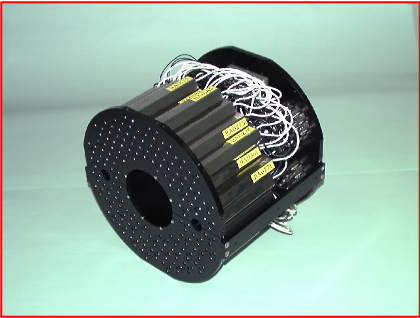
\includegraphics{mbd}
  \caption{The minimum bias detector. Originally built by Hiroshima University for HENIX, being reused for sPHENIX. }
  \label{fig:mbd}
\end{figure}

\begin{figure}[hbt!]
  \centering
  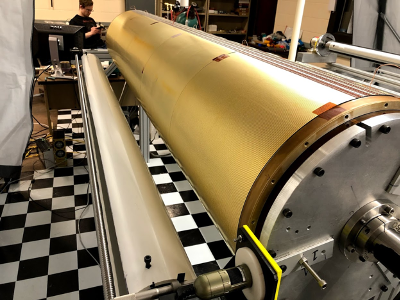
\includegraphics[width=0.49\linewidth]{innerfieldcage}
  \hfill
  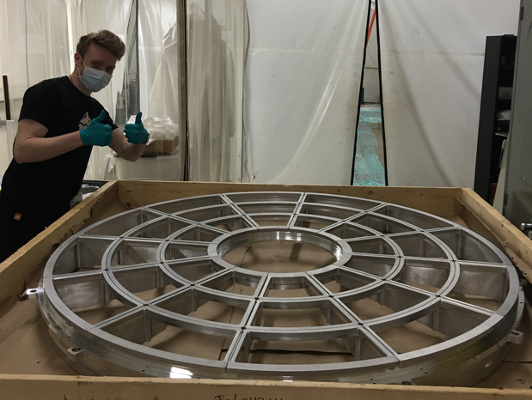
\includegraphics[width=0.49\linewidth]{wagonwheel}
  \caption{The structure --- the ``wagon wheel'' ---  which supports
    the TPC field cages, the GEMs, the readout electronics and all the
    services.  It is milled from a single billet of aluminum in order to
    eliminate joints which could allow seepage and complicate
    controlling the purity of the contained gas. }
  \label{fig:wagonwheel}
\end{figure}

\begin{figure}[hbt!]
  \centering
  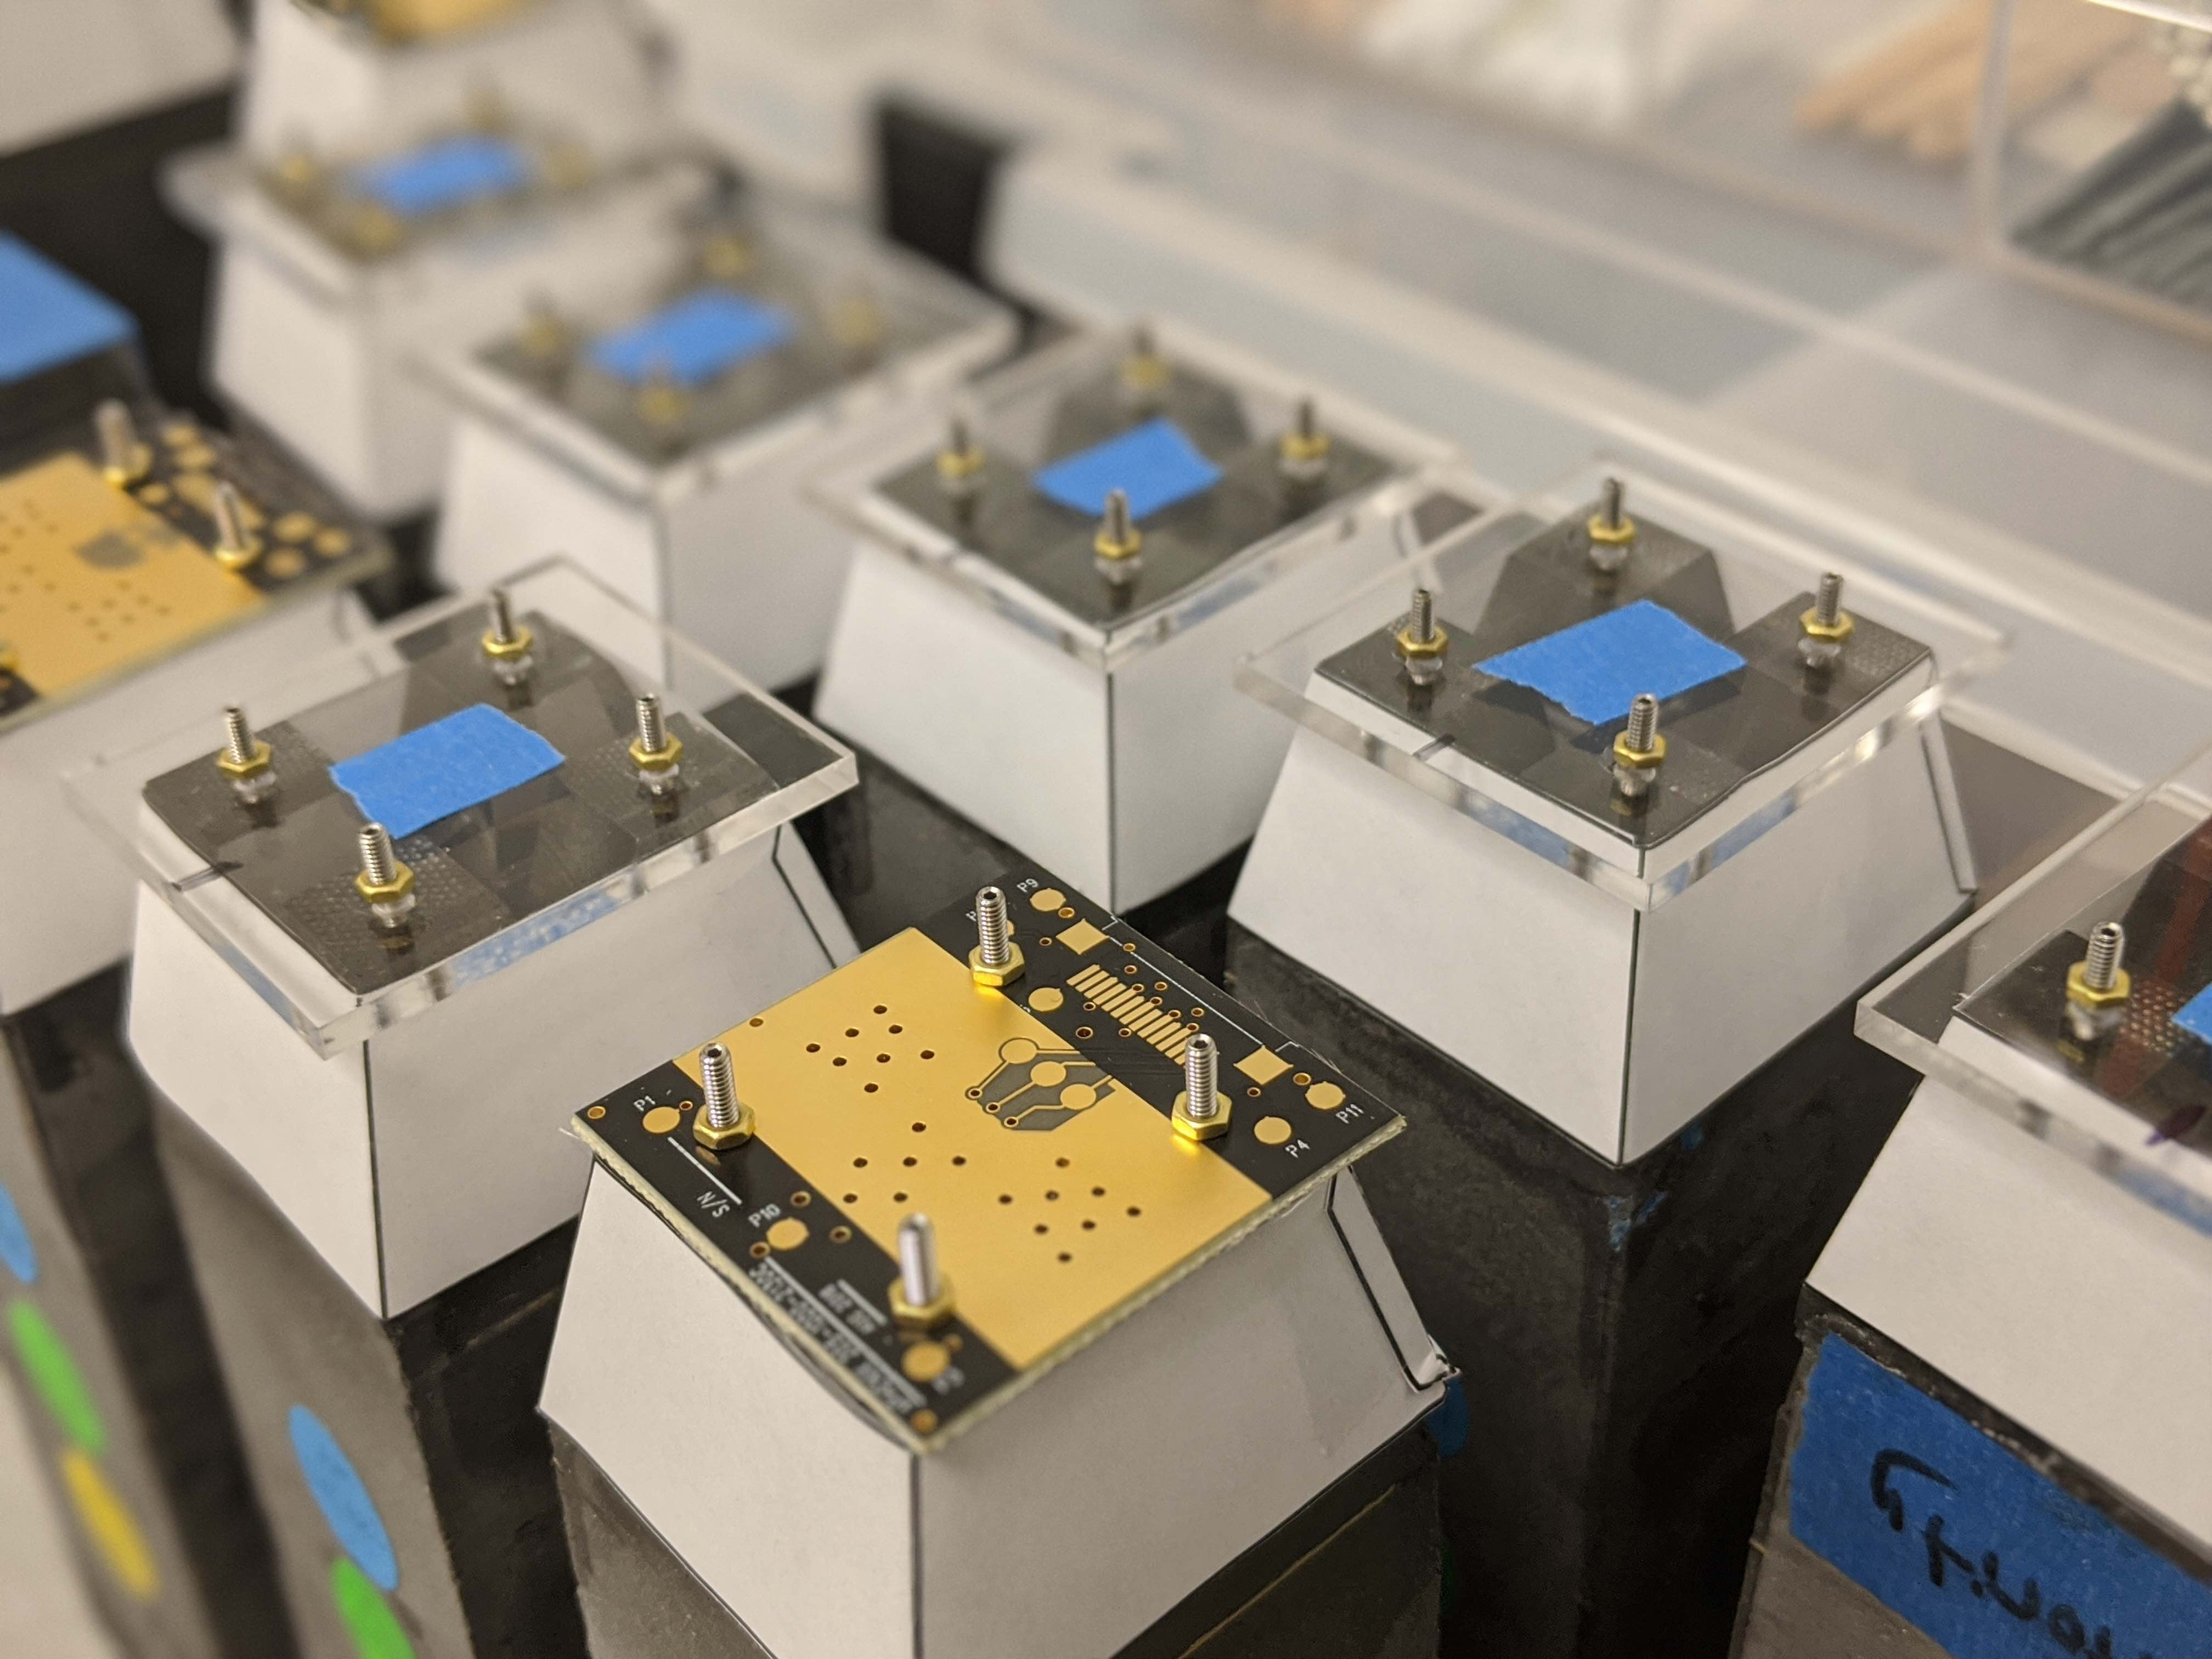
\includegraphics[width=0.49\linewidth]{emcalblocks}
  \hfill
  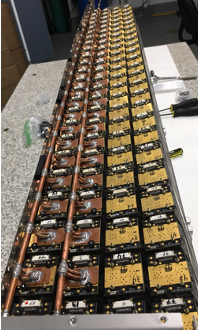
\includegraphics[width=0.49\linewidth]{sector0}
  \caption{The EMCal blocks and the assembled EMCal Sector ``0''.}
  \label{fig:emcal}
\end{figure}

\begin{figure}[hbt!]
  \centering
  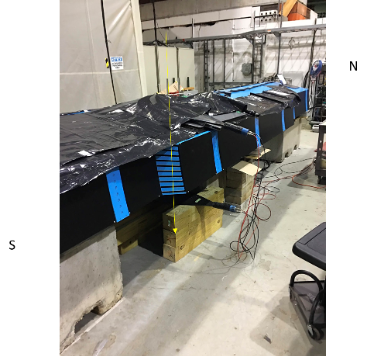
\includegraphics[width=0.49\linewidth]{ohcalsector}
  \hfill
  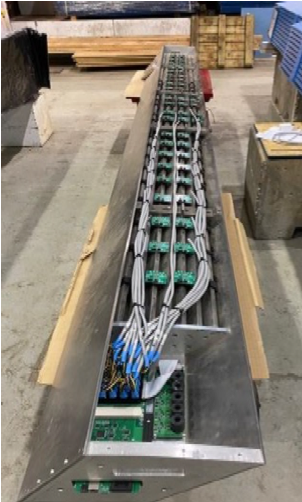
\includegraphics[width=0.49\linewidth]{ihcalsector}
  \caption{Inner and outer HCal sectors.}
  \label{fig:hcal}
\end{figure}

\begin{figure}[hbt!]
  \centering
  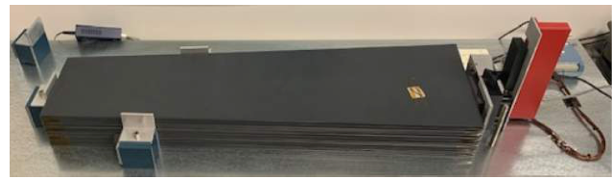
\includegraphics[width=0.75\linewidth]{tiletesting}
  \caption{Testing the HCal tiles at GSU.}
  \label{fig:tiletesting}
\end{figure}




\section{Progress since last PAC}
\label{sec:progress}

The sPHENIX MIE was granted PD-2/3 on September 20, 2019.

\begin{figure}[!hbt]
 \begin{center}
%    \includegraphics[width=0.7\linewidth]{}
        \caption{\label{fig:ohcal}All 32 sectors of the oHCal have
        been delivered and are in Bldg. 912.  A few of the sectors have
        been instrumented.}
 \end{center}
\end{figure}

\begin{figure}[!hbt]
 \begin{center}
%    \includegraphics[width=0.7\linewidth]{}
        \caption{\label{fig:ihcal}Prototype of the iHCal.  The
        construction of this is being pursued as a BNL capital project.}
 \end{center}
\end{figure}

\begin{figure}[!hbt]
 \begin{center}
%    \includegraphics[width=0.7\linewidth]{}
        \caption{\label{fig:tpc}Photos of the TPC under construction
        at Stony Brook University.}
 \end{center}
\end{figure}

\begin{figure}[!hbt]
 \begin{center}
%    \includegraphics[width=0.7\linewidth]{}
        \caption{\label{fig:intt}Staves of the silicon strip detector (INTT).}
 \end{center}
\end{figure}

\begin{figure}[!hbt]
 \begin{center}
%    \includegraphics[width=0.7\linewidth]{}
        \caption{\label{fig:mvtx}Construction photos of the MVTX.}
 \end{center}
\end{figure}


Computing needs.

Effects of COVID-19.

Relationship to EIC.

Prospects for being ready for data taking in 2023.


\chapter{Beam Use Proposal 2023-2025}
\label{chap:beam_use_proposal}

In this Chapter we detail the sPHENIX Beam Use Proposal as requested in the Associate Laboratory Director Charge for three years of running 2023-2025 assuming 24 or 28 cryo-weeks in each year.  The complete charge is reproduced in Appendix~\ref{chap:charge}.   

\section{Years 2023-2025 Proposal}

The three-year proposal is summarized in Table~\ref{tab:summary}.   The numbers correspond to 24-cryo weeks in each year with alternate numbers in parenthesis corresponding to 28-cryo weeks.    The recorded luminosity values correspond to events collected via minimum bias triggers that sample a large fraction of the inelastic cross section ($> 90\%$ in Au+Au for example).    These events are within the optimal acceptance range for the full sPHENIX detector, including the inner tracker, of $|z|<10$~cm.    
The sPHENIX inner vertex tracker MVTX is detailed in sPH-HF-2018-001 [https://indico.bnl.gov/event/4072/].   The MVTX consists of three layers with active ladder length of 271.2~mm or $\pm135.6$~mm at an average radius of 25.2, 33.4, and 41.5~mm, respectively. Therefore, collisions taking place within $|z| < 10$~cm will have optimal acceptance of $|\eta| < 1.0$ if one requires all tracks in this $\eta$ range to pass through at least two layers of the MVTX.

In 2024, we include two sets of values with the first correspond to simply recording 5~kHz of minimum bias data in \pp and \pau collisions.   The second value is with implementation of partial streaming readout (10\%-$str$) for the Time Projection Chamber (TPC) and the inner tracking detectors (MVTX, INTT).    Thus, these recorded luminosities are for the tracking only (i.e. without the calorimeters).   Details on the streaming readout are given in Chapter~\ref{chap:readout}.
The sampled luminosity values correspond to additional events that are efficiently sampled with physics specific Level-1 triggers with trigger efficiencies greater than 90\%.    In this document we detail specifically which physics channels are enhanced from these Level-1 triggers.     

\begin{table}[]
\centering
\caption{Summary of sPHENIX Beam Use Proposal for Years 2023-2025.
\label{tab:summary}}
\bigskip
\centering
\begin{tabular}{ | c | c | c | c | c | c | c | }
\hline
Year & Species & $\sqrt{s_{NN}}$ & Cyro  & Physics & Rec. Lum. & Samp. Lum. \\
     &         & [GeV]           & Weeks & Weeks   & $|z|<$10~cm & $|z|<$10~cm \\ \hline \hline

2023 & \auau   & 200 & 24 (28) & 9 (13) & 3.7 (5.7) \nb   & 4.5 (6.9) \nb  \\ \hline \hline 
2024 & $p^{\uparrow}p^{\uparrow}$     & 200 & 24 (28) & 12 (16) & 0.3 (0.4) \pb [5 kHz] & 73 (101) \pb  \\
     &                                &     &  & &  7.3 (10.1) \pb [10\%-$str$]&   \\ \hline
2024 & $p^{\uparrow}$+Au    & 200 & -- & 5 & 0.003 \pb [5 kHz]          & 0.11 \pb \\  
 &     &  &  &  &  0.01 \pb [10\%-$str$]         &   \\ \hline \hline
2025 & \auau   & 200 & 24 (28) & 20.5 (24.5) & 13 (15) \nb   & 21 (25) \nb  \\ \hline

\end{tabular}

\end{table}

The first year 2023 of running has significant commissioning time for the detector, and critically for the accelerator-detector combination, as is expected for any new major, complex collider experiment.   It is critical that this commissioning time be with \auau collisions at 200 GeV to insure a full understanding of the detector operation and performance under high occupancy conditions.   Details on the commissioning plan are given in Chapter~\ref{chap:commissioning}.    After the commissioning period, 9 (13) weeks of physics data taking are available corresponding to recorded \auau minimum bias data sets of 25 (39) billion events.   The main \auau physics run is in the third year 2025 with more than 113 (141) billion events recorded in total, i.e. 2023 and 2025 combined.
Note that for all the luminosity projections and conversions to collision rates we utilize as total inelastic cross sections:   6.8 barns, 1.7 barns, 42 millibarns for \auau, \pau, and \pp, respectively.

The second year 2024 of running provides the critical baseline measurements in \pp and \pau both at $\sqrt{s_{NN}}$=200~GeV.   The proton beam in both cases will be with transverse (vertical) polarization.  These data sets provide key baseline measurements for nuclear modification factors R$_{AA}$, R$_{pA}$, new collectivity and probes of small collision systems, as well as compelling transverse spin physics observables.    We highlight that particularly in this year, the 24-cryo week scenario is challenging since new Level-1 triggers will be commissioned and there are a significant number of cryo-weeks for switching systems.    

In the following sections, we detail the running conditions worked out with the Collider-Accelerator Division (C-AD) experts.    We then provide detailed cryo-week breakdowns for each running year, along with explicit assumptions for calculating the recorded and sampled luminosities.   

Specific details on the RHIC luminosity projections, mapping out of cryo-weeks schedules, and overall trigger/sampling calculations are given in the next Sections.

\section{RHIC Luminosity Projections}

For planning purposes in this document, we use luminosity projection numbers provided by the Collider-Accelerator Division (C-AD).   The version of the document titled 
``RHIC Collider Projections (FY 2017 –- FY 2027)'' utilized for this study is dated 21 August 2020 and utilizes knowledge gained from the Run-15 p+p and p+Au at 200~GeV running and the Run-16 \auau at 200 GeV running.   The document is available at:

\vspace{0.1in}
{\color{blue}{http://www.rhichome.bnl.gov/RHIC/Runs/RhicProjections.pdf}} 
\vspace{0.1in}

Note that the document linked above is periodically updated, so note the date tag.  In general, C-AD provides a minimum and maximum luminosity per week for each running period, as well as the fraction of collisions within a given z-vertex range. For calculating the integrated luminosity, we assume a ramp-up curve and then a steady-state physics running at the mean of the minimum and maximum in both luminosity and z-vertex fraction within $|z|<$10~cm (where a minimum and maximum are given).  

A critical part of the sPHENIX run plan is to have a non-zero crossing angle between the beams.    We detail the crossing angle reasoning, implications, and quantitative analysis in Chapter~\ref{chap:cad}.    

For this plan, we assume an sPHENIX up-time (i.e. the fraction of time when collisions are available that sPHENIX is taking data with high livetime) of 0.60 for the first two years of running (2023 and 2024) since the detector is being commissioned for new collision systems and new Level-1 triggers are being brought online, and 0.80 for subsequent running (2025).   These up-time values fold in the expected deadtime of the data acquisition system - of order 90-95\%.

RHIC C-AD projections for time in store (i.e. RHIC up-time) vary slightly with most of the projected values around 0.60. It is notable that C-AD projections are for a nominal 8 hour store; however, a more optimal store length may be found in future running at closer to 5 hours.

\section{Cryo-Weeks}

For mapping out a run plan, we state both cryo-weeks for a running period and also physics data taking weeks, i.e. when Physics Running is declared by C-AD.   The guidance from C-AD is that there is a 0.5 week ``cool down from 50 K to 4 K'', then a 2.0 week ``set-up mode'' for the specific collision species, and then a 0.5 week ``ramp-up''.   If switching species, there is again a 2.0 week ``set-up'' and 0.5 week ``ramp-up''.    Lastly, at the end of the running period, there is a 0.5 ``warm-up from 4 K to 50 K''.  

In addition, we assume that in the first, second and third weeks of declared Physics Running, one achieves 25\%, 50\%, and then 75\% of the luminosity target, with subsequent weeks at 100\% (again of the mean of the minimum and maximum).

Following the detailed C-AD guidance, we present the cryo-week break downs for the 24 (28) week scenarios.   
The break-downs are shown for 2023 in Table~\ref{tab:cryoplan2023}, for 2024 in Table~\ref{tab:cryoplan2024}, and for
2025 in Table~\ref{tab:cryoplan2025}.

\begin{table}
\centering
\begin{tabular}{ | c | l | }
\hline
Weeks & Designation \\ \hline
0.5  & Cool Down from 50 K to 4 K \\ \hline
2.0  & Set-up mode 1 (Au+Au at 200 GeV) \\ \hline
0.5  & Ramp-up mode 1 (8 h/night for experiments) \\ \hline
11.5  & sPHENIX Initial Commission Time \\ \hline
9.0 (13.0) & Au+Au Data taking (Physics) \\ \hline
0.5  & Controlled refrigeration turn-off \\ \hline \hline \hline
24.0 (28.0) & Total cryo-weeks \\
\hline
\end{tabular}
\caption{Year 2023 run plan for 24 (28) cryo-weeks with \auau 200~GeV collisions.\label{tab:cryoplan2023}}
\end{table}

\begin{table}
\centering
\begin{tabular}{ | c | l | }
\hline
Weeks & Designation \\ \hline
0.5  & Cool Down from 50 K to 4 K \\ \hline
2.0  & Set-up mode 1 (p$^{\uparrow}$p$^{\uparrow}$ at 200 GeV) \\ \hline
0.5  & Ramp-up mode 1 (8 h/night for experiments) \\ \hline
12.0 (16.0) & Data taking mode 1 (p$^{\uparrow}$p$^{\uparrow}$ Physics) \\ \hline
1.0  & Move DX magnets \\ \hline
2.0  & Set-up mode 2 (p$^{\uparrow}$+Au at 200 GeV) \\ \hline
0.5  & Ramp-up mode 2 (8 h/night for experiments) \\ \hline
5.0 & Data taking mode 2 (p$^{\uparrow}$+Au Physics) \\ \hline
0.5  & Controlled refrigeration turn-off \\ \hline \hline \hline
24.0 (28.0) & Total cryo-weeks \\
\hline
\end{tabular}
\caption{Year 2023 run plan for 24 (28) cryo-weeks with p$^{\uparrow}$p$^{\uparrow}$ and p$^{\uparrow}$+Au 200~GeV collisions.\label{tab:cryoplan2024}}
\end{table}

\begin{table}
\centering
\begin{tabular}{ | c | l | }
\hline
Weeks & Designation \\ \hline
0.5  & Cool Down from 50 K to 4 K \\ \hline
2.0  & Set-up mode 1 (Au+Au at 200 GeV) \\ \hline
0.5  & Ramp-up mode 1 (8 h/night for experiments) \\ \hline
20.5 (24.5) & Au+Au Data taking (Physics) \\ \hline
0.5  & Controlled refrigeration turn-off \\ \hline \hline \hline
24.0 (28.0) & Total cryo-weeks \\
\hline
\end{tabular}
\caption{Year 2025 run plan for 24 (28) cryo-weeks with \auau 200~GeV collisions.\label{tab:cryoplan2025}}
\end{table}

\section{Sampled versus Recorded Luminosity}

In the \auau 200~GeV case, the physics will predominately come from {\bf recorded} minimum bias collisions.   This data will be selected by the Level-1 trigger via the MBD that samples approximately 90\% of the inelastic cross section.   Additional physics may be ``sampled'' with rare event triggers, for
example high-\pt direct photons, where the trigger rejection is very high even in central \auau events.   All physics projections are based on the recorded luminosity in \auau unless otherwise stated.     
The key requirements to achieve these recorded event sets are (1) the sPHENIX Data Acquisition Level-1 accept rate of 15 kHz with livetime from 90-95\%, (2) the luminosity corresponds to a rate of collisions within $|z|<$10 cm during the store above 15 kHz, and (3) maintaining the sPHENIX and RHIC uptime projections. 
As shown in Figure~\ref{fig:auaulumcurves}, the projected \auau collision rate within $|z|<10$~cm exceeds the 15~kHz minimum bias recording capacity for most all of a five-hour store.   There is a factor of order 1.5-2.5 depending on the year that can be additionally sampled by very selective physics triggers in \auau.

\begin{figure}
\centering
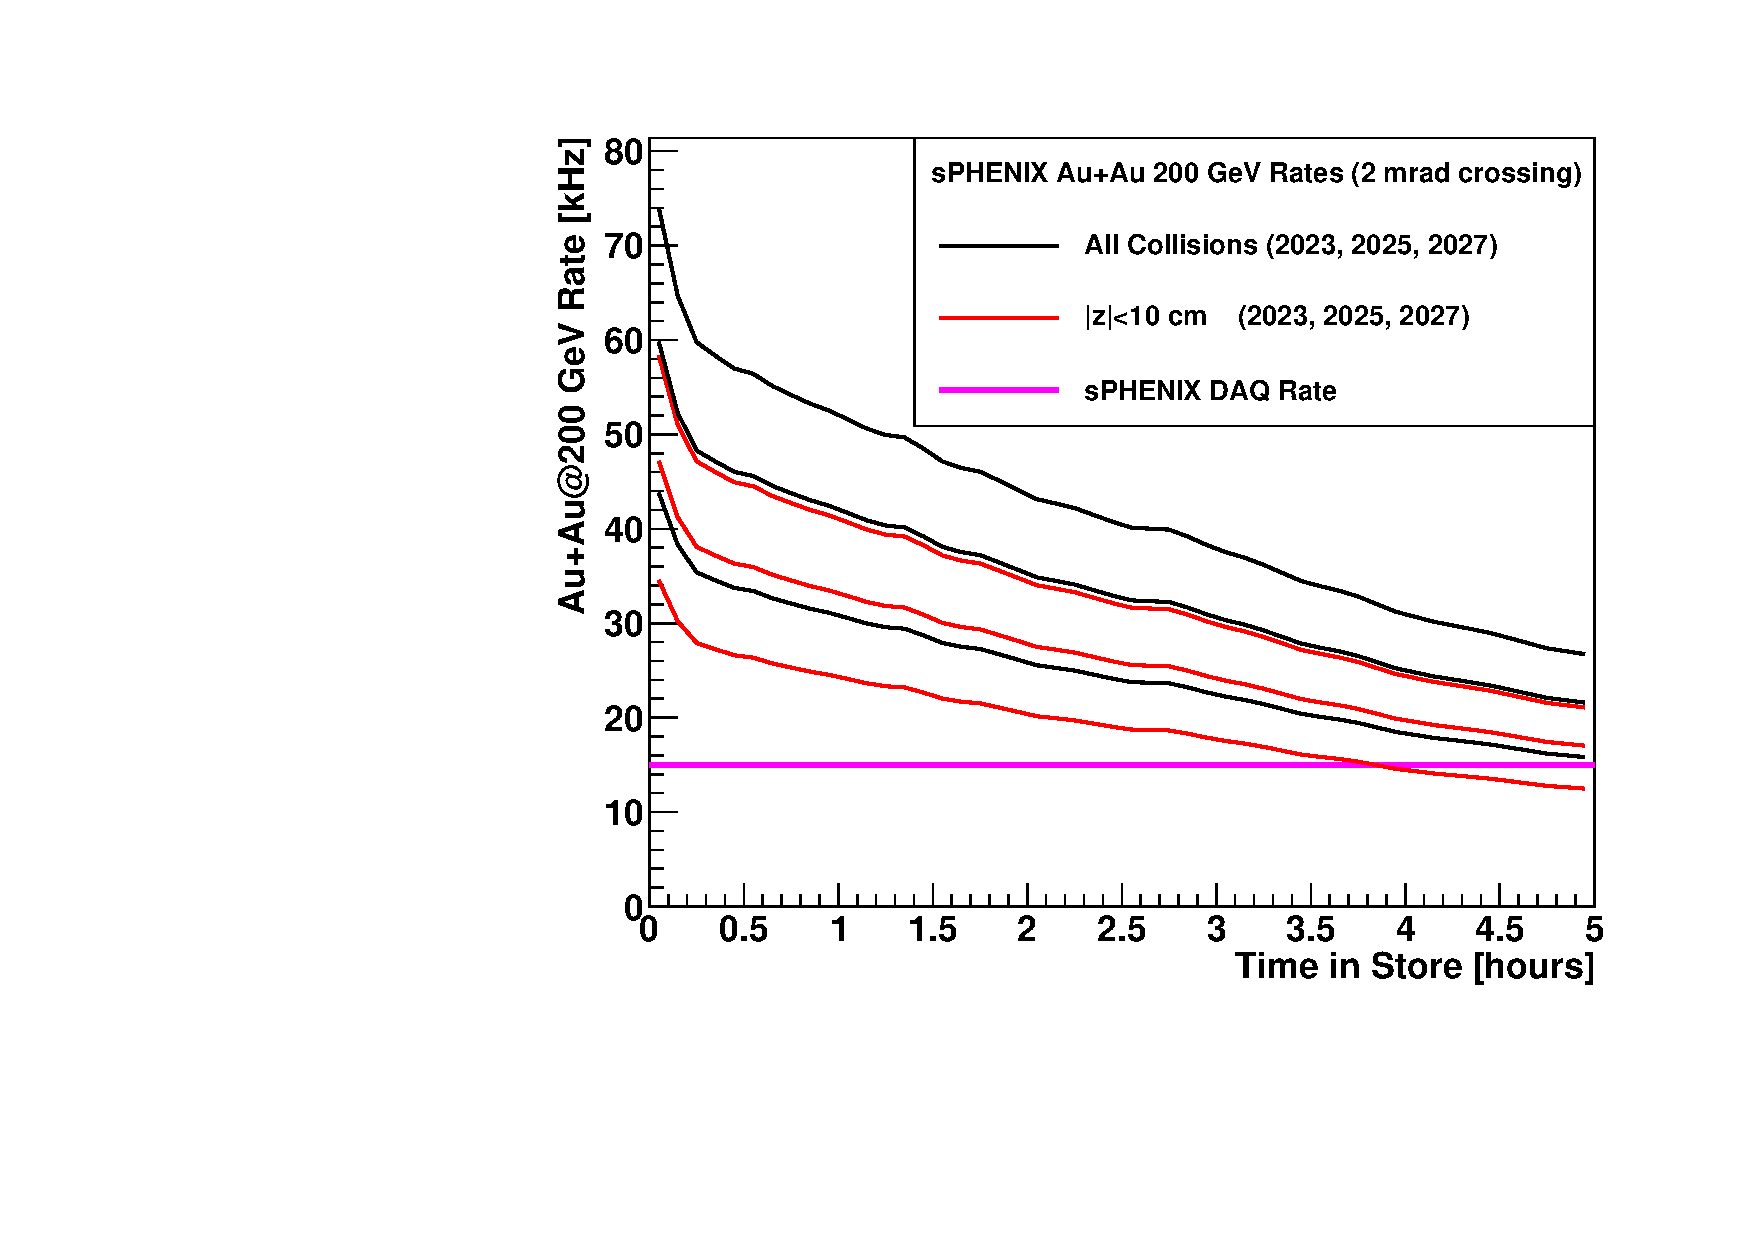
\includegraphics[width=0.70\linewidth]{figs/figure_auauratestore_2mrad.pdf} 
\caption{Estimated \auau at 200 GeV collision rate as a function of time in store for all collisions (black) and collisions within $\pm$ 10 cm (red).  The bottom to top set of curves in each color are for the mean luminosity and fraction within $\pm$ 10 cm for the C-AD projections labeled in their document as 2023, 2025, 2027.   Also shown as a magenta band is the sPHENIX Data Acquisition Level-1 accept rate of 15~kHz for reference.
\label{fig:auaulumcurves}}
\end{figure}

In the \pp and \pau case, the physics will predominantly come from {\bf sampled} Level-1 triggered events utilizing photon, electron (e.g. from Upsilon decays), hadron, and
jet triggers.  Thus, the key value is the sampled luminosity for these physics channels.   Note that some observables such as lower \pt hadrons (and in particular heavy-flavor hadrons $D$, $\Lambda_{c}$, $B$) do not have effective Level-1 physics triggers.    Thus, in these cases the recorded luminosity is crucial.    We have nominally allocated 5~kHz out of the 15~kHz Level-1 trigger rate for \pp and \pau minimum bias collection.   A critical addition is the streaming capability for the tracking detectors which enables much larger minimum bias data sets (without calorimeter readout).

Trigger algorithms have been developed and tested using the EMCal for single photons (typically with \pt greater than 10 Gev/c) and for electrons (from Upsilon decays typically with \pt greater than 3-4 GeV/c).  In addition, trigger algorithms using the combined EMCal and HCal information have been developed for selecting jets and single hadrons.    At the highest \pp interaction rates, rejection factors of order 5000-10,000 are needed to result in a 1-2 kHz bandwidth allocation for a given trigger channel.    Full {\textsc{GEANT-4}} simulations with {\textsc{HIJING}} \pp and \pau events have been used to document the trigger efficiencies and rejection factors for all Level-1 algorithms.
One example set of calculations for jet triggers is shown in Figure~\ref{fig:trigger} indicating good efficiency and rejection factors above the required level.

\begin{figure}
    \centering
    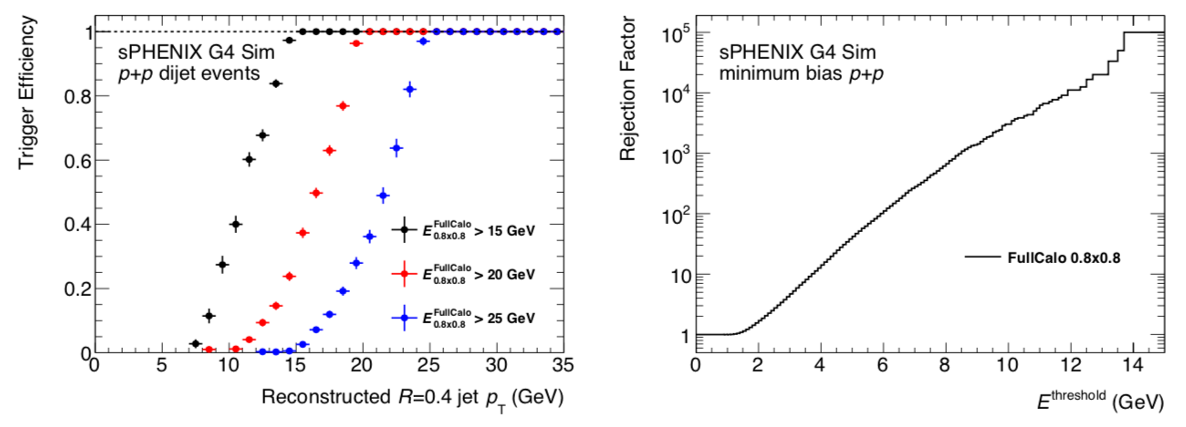
\includegraphics[width=\linewidth]{figs/figure_sphenix_jettrigger.png}
    \caption{sPHENIX full {\textsc{GEANT-4}} simulations with {\textsc{HIJING}} \pp events run through the jet Level-1 trigger emulator with efficiencies (left) and rejection factors (right).}
    \label{fig:trigger}
\end{figure}

It is useful to put the data sets for the three proposed systems (\pp, \pau, \auau) into context, and here we compare the relative statistics for high $p_T$ jets.
For \auau minimum bias events, the average number of binary collisions is 
$\left< N_{coll} \right> \approx 250$.   
Similarly, for \pau the $\left< N_{coll} \right> = 4.7$.
Table~\ref{tab:ncoll} details the number of relevant events recorded or sampled for measuring high $p_T$ jets.    We highlight that the \auau sample with an order of magnitude more effective $p+p$ collisions sampled will be divided into multiple centrality bins and jet quenching will reduce the statistics are high $p_T$.   Overall this is a good balance of cold and hot system measurements.

\begin{table}[]
    \centering
    \begin{tabular}{|c|c|c|c|}\hline
         Species & Year 1-3 Total & $\left< N_{coll} \right>$ & Effective-\pp \\ \hline\hline
         \pp & 101~\pb (sampled) & 1 & $4 \times 10^{12}$\\ \hline
         \pau & 0.11~\pb (sampled) & 4.7 & $0.9 \times 10^{12}$ \\ \hline
         \auau & 20.7~\nb (recorded) & 250 & $35 \times 10^{12}$ \\ \hline
    \end{tabular}
    \caption{Comparison from the full data sets from Years 2023-2025 assuming the 28 cryo-week scenarios for the three systems \pp, \pau, \auau.}
    \label{tab:ncoll}
\end{table}

 







\chapter{C-AD Guidance}
\label{chap:cad}

For planning purposes in this document, we use luminosity projection numbers provided by the Collider-Accelerator Division (C-AD).   The version of the document titled 
``RHIC Collider Projections (FY 2017 –- FY 2027)'' utilized for this study is dated 12 August 2020 and utilizes knowledge gained from the Run-15 p+p and p+Au at 200~GeV running and the Run-16 \auau at 200 GeV running.   The document is available at:

\bigskip
{\color{blue}{http://www.rhichome.bnl.gov/RHIC/Runs/RhicProjections.pdf}} 
\bigskip

Note that the document linked above is periodically updated, so note the date tag.  In general, C-AD provides a minimum and maximum luminosity per week for each running period, as well as the fraction of collisions within a given z-vertex range. For calculating the integrated luminosity, we assume a ramp-up curve and then a steady-state physics running at the mean of the minimum and maximum in both luminosity and z-vertex fraction within $|z|<$10~cm (where a minimum and maximum are given).  

\section{Crossing Angle}

The original C-AD projections from three years ago for \auau 200~GeV collision rate as a function of time-in-store for the years 2023, 2025, and 2027 are shown in Figure~\ref{fig:auaulumcurves} (left).    The black curves are the collision rate for interactions at any longitudinal $z$ vertex position, while the red curves are the collision rate for interactions with $|z|<$10~cm.    The magenta curve corresponds to the design specified 15~kHz sPHENIX Level-1 trigger accept rate.
These projections are with zero crossing angle between the beams.   

The sPHENIX optimal acceptance for the inner tracking detectors is with collisions within $|z|<$10~cm.   Thus, it is clear that a majority of the collisions in this scenario have highly sub-optimal tracking acceptance.   In principle these collisions far outside the optimal still could be used for calorimeter-only physics measurements (e.g. high $p_{T}$ photons and calorimetric jets) -- however, one would not have good acceptance to measure fragmentation functions, medium response via tracks in these events.    There is a significant down side to the very large collision rate outside of $|z|<$10~cm.   These collisions still leave hits in the TPC and thus substantially increase ion back-flow (IBF) and fluctuations in the IBF.   This additional charge is corrected for and at the same time gets more and more challenging and eventually degrades the momentum resolution and track finding efficiency.    Additionally, component of sPHENIX including the calorimeter silicon photo-multipliers (SiPMs) are susceptible to radiation damage over time.   These additional collisions significant increase the overall time-integrated radiation load on the detector.

Therefore, after detailed discussions with C-AD, sPHENIX plans to run with a nominal beam crossing angle of 2 milliradians in \auau collisions.    C-AD has included collision rate information at beam crossing angles of 0, 1, and 2 milliradians in their projections document.    Figure~\ref{fig:auaulumcurves} (right) shows the collision rate as a function of time in store for a nominal 2 milliradian crossing angle.   There is a modest reduction in collision rate within $|z|<$10~cm; however, it still exceeds the 15~kHz Level-1 accept rate throughout the store.   What is most noticeable is the reduction by almost a factor of $\times$3 in total collision rate.   This effectively translated into a factor of $\times$3 lower radiation load on the detector and $\times$3 lower charge deposition in the TPC.   Small optimizations around the 2 milliradian value may be possible; for the purposes of this document we have consistently used this crossing angle for \auau projections.

\begin{figure}
\centering
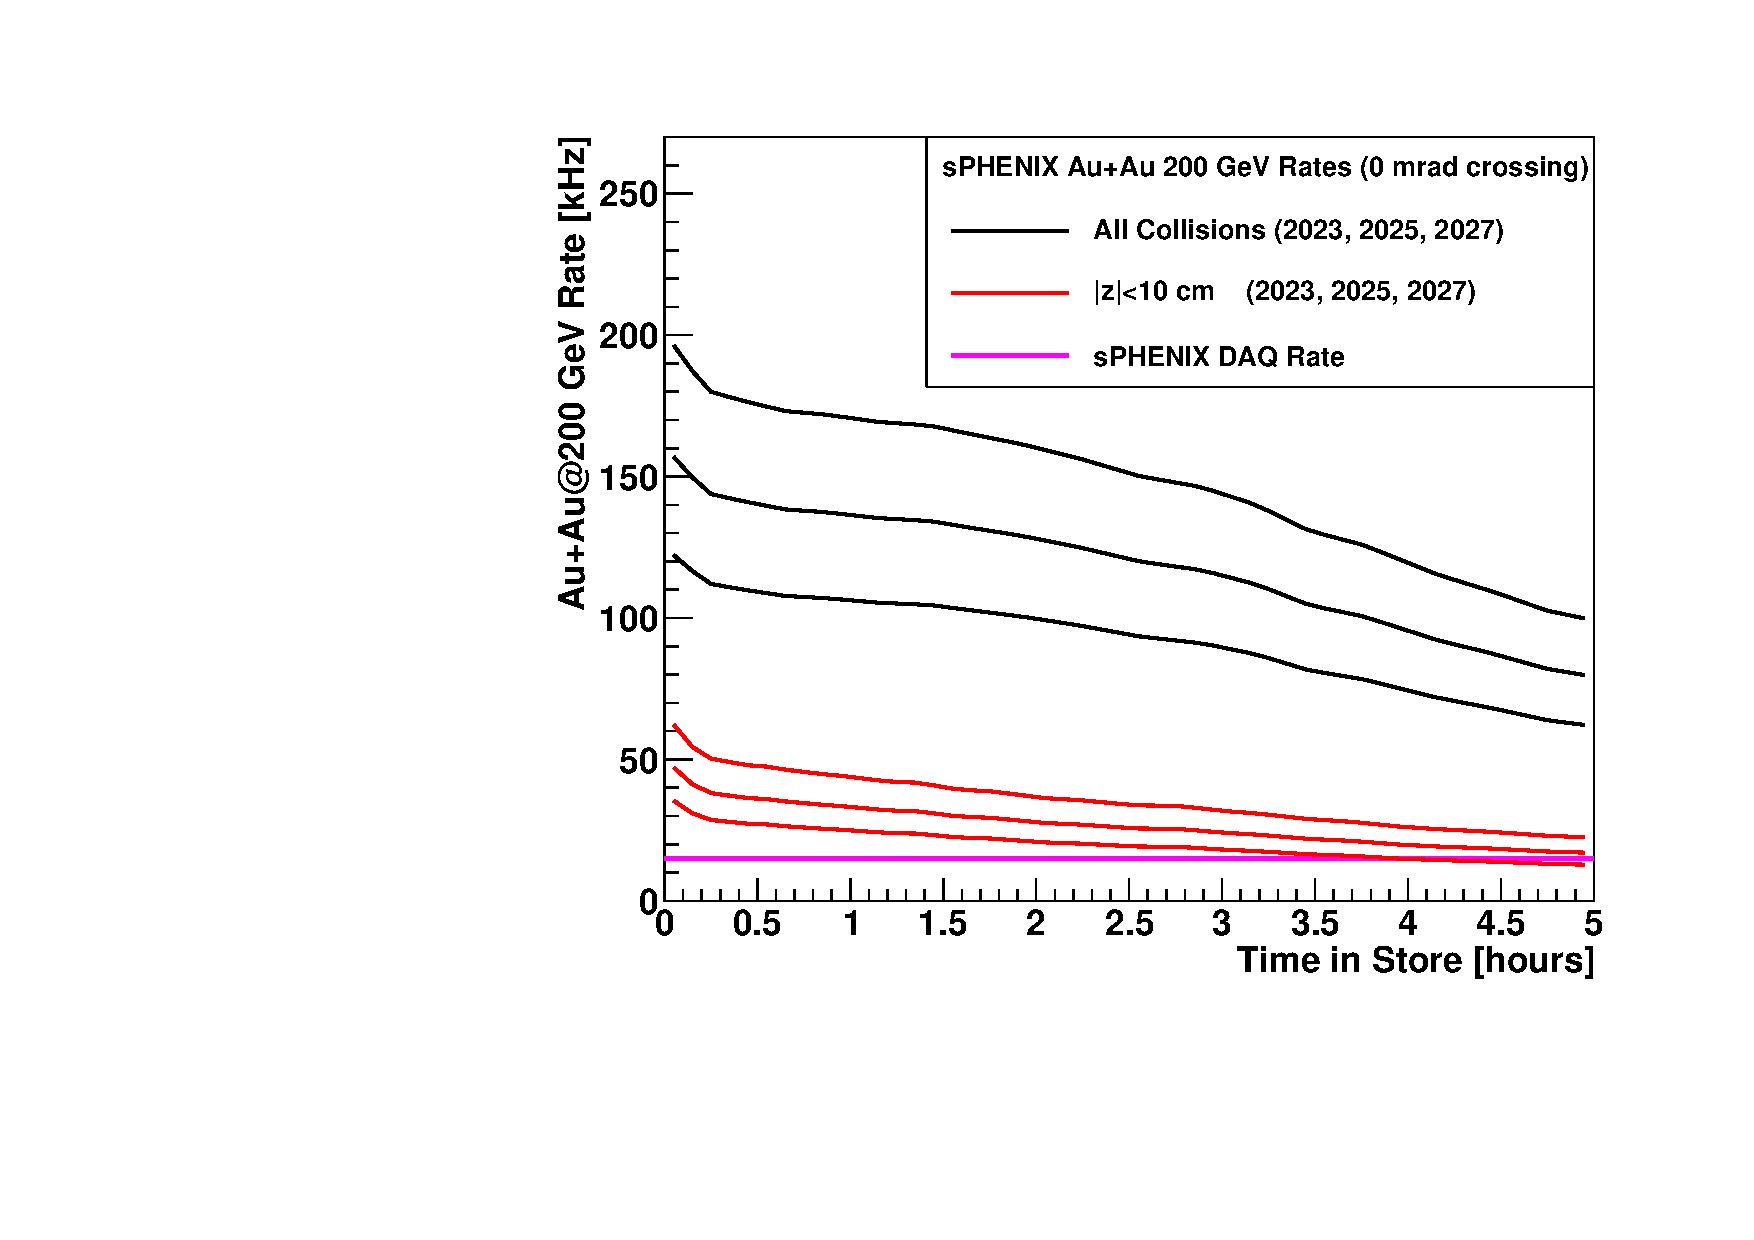
\includegraphics[width=0.47\textwidth]{figs/figure_auauratestore_0mrad.pdf}
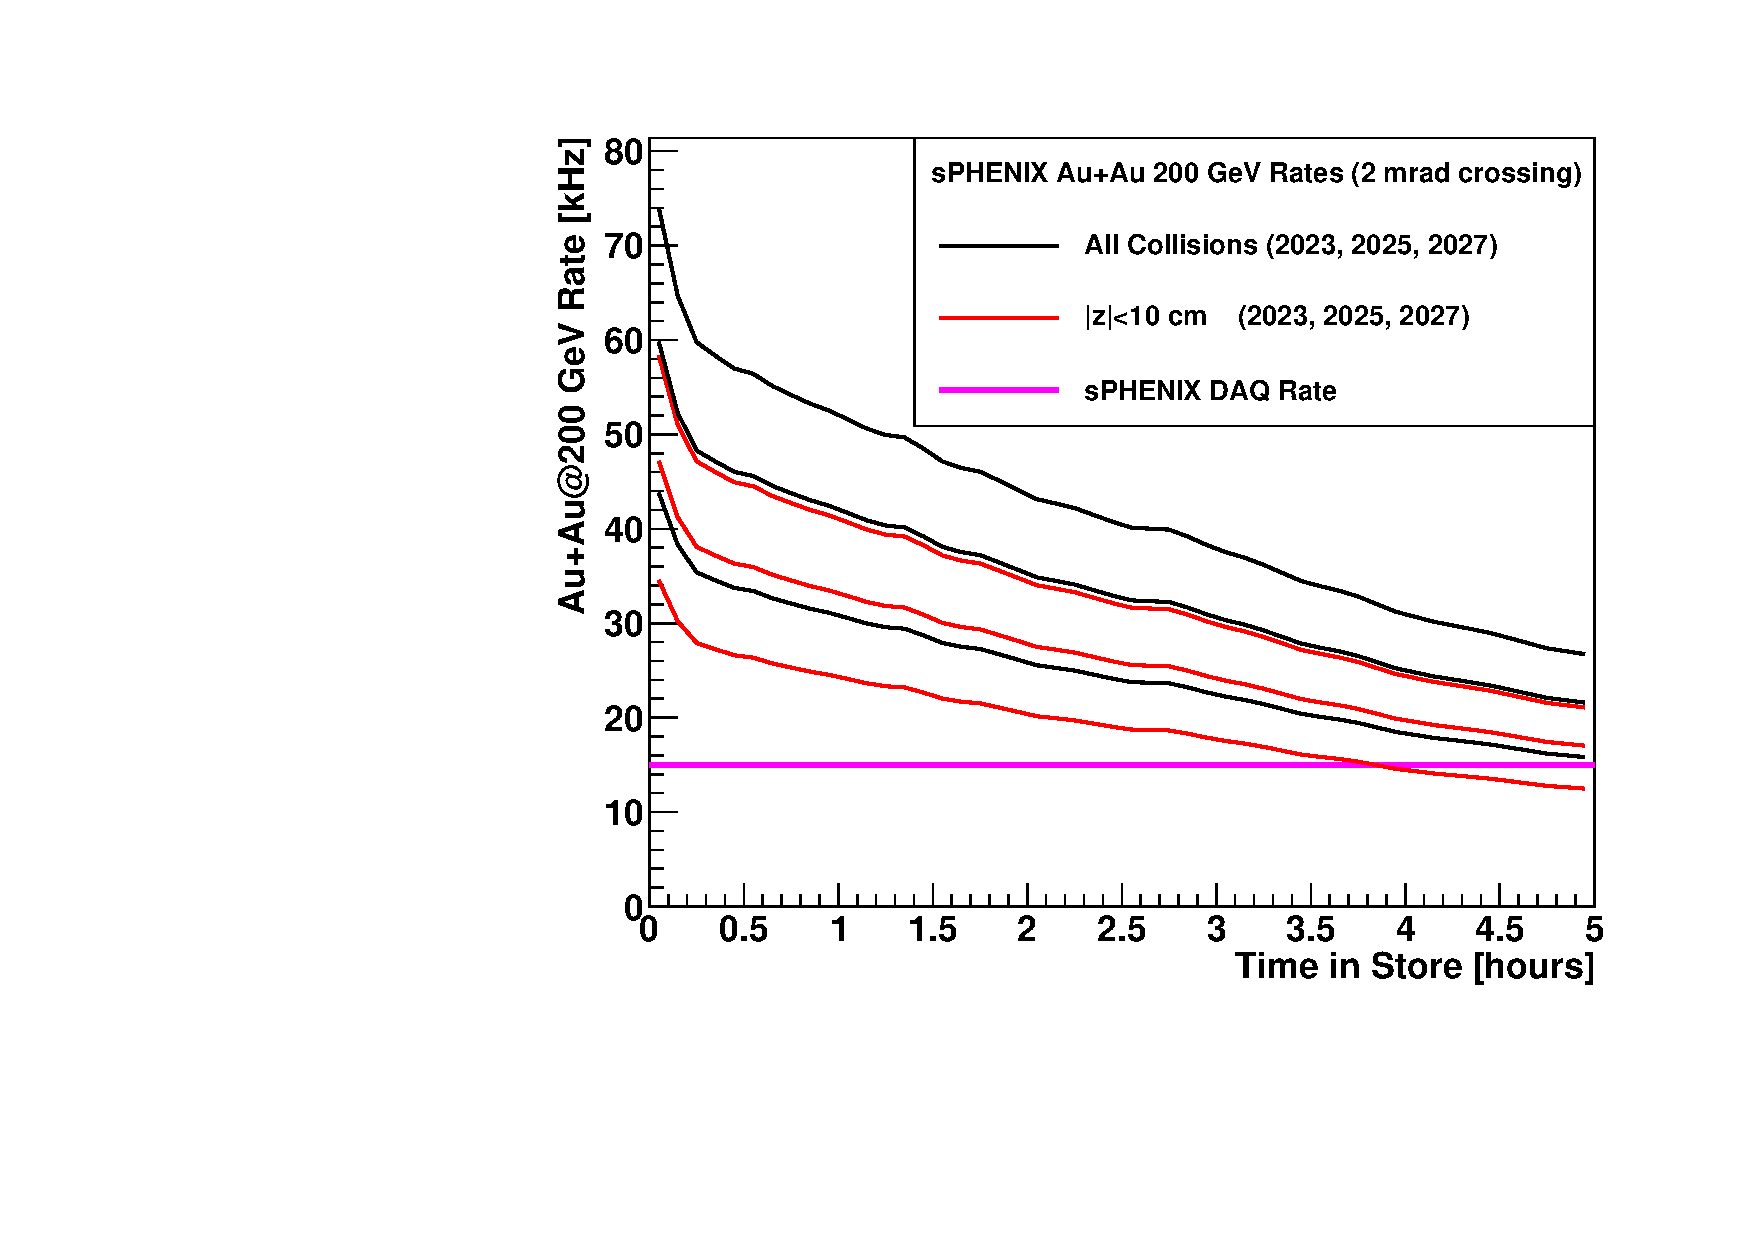
\includegraphics[width=0.47\linewidth]{figs/figure_auauratestore_2mrad.pdf}
\caption{(left) Estimated \auau at 200~GeV collision rate as a function of time in store for all collisions (black) and collisions within $\pm$ 10 cm (red).   The bottom to top set of curves in each color are for the C-AD projections in their document corresponding to 2023, 2025, 20278.
Also shown as a magenta band is the sPHENIX data acquisition rate of 15~kHz for reference.
These projections are with zero crossing angle between the beams. 
(right)
The same calculated quantities, now updated by C-AD, and for a 2 milliradian crossing angle between the beams.
\label{fig:auaulumcurves}}
\end{figure}

Similar issues of acceptance and radiation load / IBF have to be balanced for \pp and \pau running.   The current proposal is to run with the same 2 milliradian crossing angle for these systems as well.    We highlight that in \pp and \pau running, the larger collision rate with lower track multiplicities may lead to small IBF fluctuations since the collisions are spread out in $z$ vertex and there are more throws of the dice to average out relative to a smaller number of \auau collisions with highly variable multiplicity.     It may be that there is thus a somewhat smaller crossing angle that will be optimal for the smaller collision systems.    

\section{Summary of Projected Luminosities} 

Wolfram Fischer and C-AD have provided a {\textsc{Mathematica}} notebook for estimating the collision rate and z-vertex collision distribution as a function of beam crossing angle.  After confirming values with C-AD, we include the generated set of results here for completeness.    

\begin{figure}[h!]
    \centering
        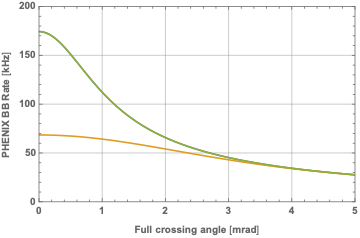
\includegraphics[width=0.7\linewidth]{figs/figure_cad1_prelim.png}  
    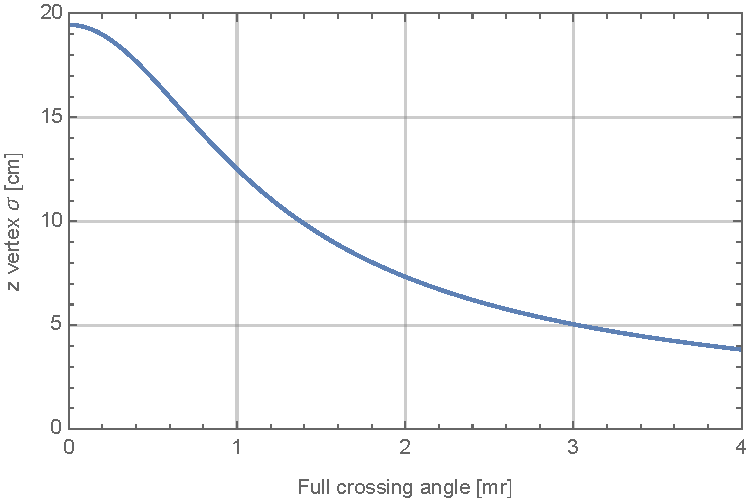
\includegraphics[width=0.62\linewidth]{figs/auau200-2023-202008131-z.pdf}
    \caption{C-AD {\textsc{Mathematica}} file generated \auau collision luminosity (left) and $z$-vertex Gaussian $\sigma$ (right) as a function of beam crossing angle.}
    \label{fig:mathauau1}
\end{figure}

\begin{figure}[h!]
    \centering
        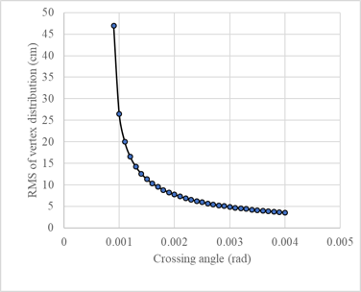
\includegraphics[width=0.47\linewidth]{figs/figure_cad2_prelim.png}  
    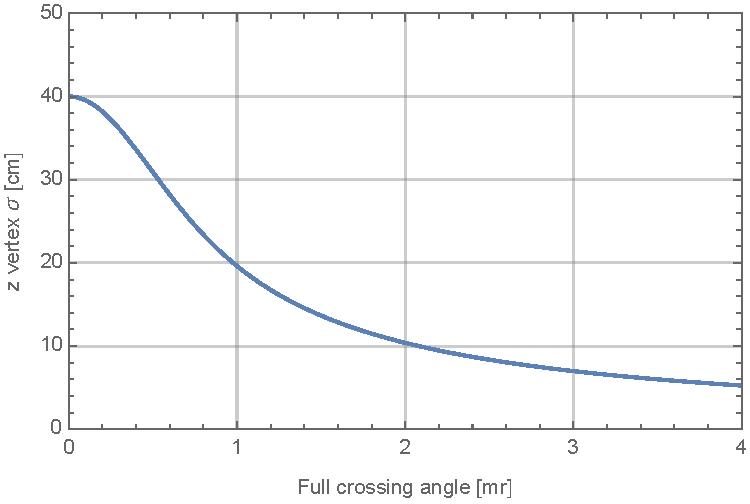
\includegraphics[width=0.43\linewidth]{figs/pp200-2023-202008131-z.pdf}
    \caption{C-AD {\textsc{Mathematica}} file generated \pp collision luminosity (left) and $z$-vertex Gaussian $\sigma$ (right) as a function of beam crossing angle.}
    \label{fig:mathpp1}
\end{figure}

\begin{figure}[h!]
    \centering
        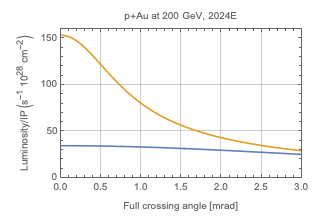
\includegraphics[width=0.47\linewidth]{figs/figure_cad3_prelim.png}  
    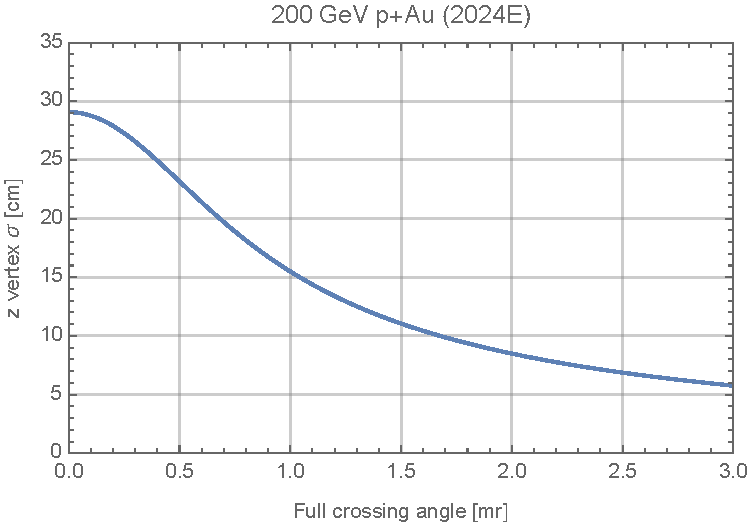
\includegraphics[width=0.43\linewidth]{figs/pau200-2024-z-202008190.pdf}
    \caption{C-AD {\textsc{Mathematica}} file generated \pau collision luminosity (left) and $z$-vertex Gaussian $\sigma$ (right) as a function of beam crossing angle.}
    \label{fig:mathpau1}
\end{figure}


\chapter{sPHENIX Commissioning}
\label{chap:commissioning}

As expected with any new collider detector, there will be significant
commissioning time required in order to be ready for physics quality
data.  The sPHENIX project and collaboration teams have taken this
task seriously with detailed input from the detector subsystems and
the sPHENIX Physics Working Groups.  We detail the initial
commissioning plan and timeline for 2023 in this Chapter.

\section{Timeline}

\renewcommand{\arraystretch}{1.9}
\addtolength{\tabcolsep}{-0.5pt}
\begin{table}[]
  \caption{\label{tab:commision}Timeline for sPHENIX commissioning
    period in 2023, the first year of operation.}
    \centering
    \begin{tabular}{S[table-format=2.1]l} \toprule
        {Weeks} &  Details \\ \midrule
        1.5 & low rate, 6 bunches \\ 
        2.0 & low rate, 111 bunches, MBD L1 timing \\ 
        1.0 & low rate, crossing angle checks \\ 
        1.0 & low rate, calorimeter timing \\ 
        4.0 & medium rate, TPC timing, optimization \\
        2.0 & full rate, system test, DAQ throughput \\ \bottomrule
        11.5 & {\bf total} 
    \end{tabular}
\end{table}

Commissioning sPHENIX with beams in RHIC should progress in stages
with gradually increasing luminosity.  \auau collisions are necessary
for commissioning due to the high multiplicities which can be used to
assess the detector performance with larger occupancy.  We note that
installation of the sPHENIX inner silicon detectors takes 2--3 weeks
and thus these sensitive detectors will be installed ahead of the 2023
running period for system debugging and cosmic ray data taking.  The
presence of the full detector configuration means that very careful
monitoring of luminosity and beam conditions is essential to maintain
stable operations and minimize detector risk.  Thus, the sPHENIX
experiment will require very careful coordination with C-AD including
potential accelerator down times for access.  A summary of the
projected initial commissioning timeline is shown in
Table~\ref{tab:commision}.

\section{Commission Period Details}

For the purposes of this Beam Use Proposal, we include a very brief
summary of the timeline as given.  Except for initial stores with six
bunches, operation with the maximum number of bunches (111) is
preferable to reducing luminosity by reducing the number of filled
bunches because it allows sPHENIX to commission as it plans to run.
Initial stores should be zero crossing angle, both to begin operations
with stores less likely to be lost as well as to provide a direct
comparison of vertex distribution between crossing angles of zero and
the nominal 2 milliradians.

The superconducting solenoid should be operating at full field during
the commissioning.  The minimum bias detector (MBD) gains are reduced
by the magnetic field, and so tuning should take place at the field
planned for physics operation.

\begin{itemize}

\item Initial studies will require 1.5 weeks of stores with six
  bunches, zero crossing angle, and a collision rate of up to 2~kHz.
  These collisions will be used for an initial tune-up of timing and
  the MBD trigger.  A simple ''blue logic'' trigger may be used
  initially for timing.  Several days may be required before we can
  fully operate the detector to provide time for use of diagnostic
  instrumentation and to process data, but the stores can be kept in
  RHIC as long as practical.

\item The next period will consist of two weeks of stores with 111
  bunches, zero crossing angle, and a collision rate of 1--5~kHz.
  These stores will be used for optimizing the MBD Level-1 (L1)
  trigger, which may require additional timing adjustments of the
  trigger primitives.  This phase will also require relatively short
  periods of data taking followed by analysis and diagnostics.  Near
  the end of this period, the calorimeters could be turned on, and
  timing them in could be attempted if it was not already done during
  the previous period.  Operation during the second week will employ
  the planned crossing angle.  This should allow the first measurement
  of the vertex distribution with the planned crossing angle and
  begin any optimization of the ramp that may be necessary while the
  tracking detectors, including the two inner silicon detectors, are
  turned off.

\item We estimate that it will take a week of machine studies at this
  point to optimize the beam crossing angle.  Careful coordination
  between sPHENIX and RHIC operations will be important in this stage.

\item The next week will consist of stores with 111 bunches and
  non-zero crossing angle, and will be used for calorimeter timing and
  tuneup.  The crossing angle will allow us to assess the radiation
  dosage to the silicon photo-multipliers (SiPMs) by measuring the
  leakage current with the monitoring system.

\item The next phase will consist of four weeks of stores with 111
  bunches, non-zero crossing angle, and a collision rate of 1--5 kHz.
  These stores will be used for initial operation of the tracking
  detectors, beginning with the TPC.  The minimum bias trigger,
  developed in the previous weeks, will be used to trigger the
  detector.  It may be useful during this phase to operate with zero
  magnetic field and/or very low luminosity for periods of time in
  order to collect data which can be used to align the tracking
  detectors and characterize track distortions.  Some additional time
  may be necessary for data taking at zero field in order to change
  the MBD high voltage for zero field.

\item The next two weeks will involve stores with 111 bunches,
  non-zero crossing angle, and an increasing rate of minimum bias
  collisions, culminating in fills that provide 15--20~kHz of
  collisions in order to stress test the data acquisition system under
  target running conditions.

\end{itemize}

At the end of this 11.5 week commissioning plan, the detector should be
ready to take data from all detectors, triggered according to plan for
\auau, at the design rate of the data acquisition system.  Of course,
producing data of publication quality requires more analysis than can
be brought to bear while the collaboration is commissioning the
apparatus, but it is crucial to develop monitoring software which
allows us to quickly assess the quality of data as we take it.  We
note that such commissioning time always has a significant uncertainty,
and run time flexibility in this first year of running will be
required.

Additional trigger specific commissioning time is needed for each new
collision species, particularly the physics-selective Level-1 triggers
in the 2024 \pp and \pau running.  This commissioning time is built
into the ramp up calculation for integrated luminosities in these
periods.  We highlight that we have also included a 60\% up-time for
the sPHENIX detector in 2023 and 2024, and then an 80\% up-time in
2025.

\chapter{Upgrades of the sPHENIX Readout}
\label{chap:readout}

In this Chapter we detail two potential upgrades of the sPHENIX data
acquisition and readout system of modest cost that would significantly
enhance the original physics program.  The first is a streaming
(rather than triggered) readout of the tracking detectors (MVTX, INTT,
and TPC) which could be available at 10\% capacity for the 2024 run
and at 100\% capacity for running in 2026--2027 should that
opportunity arise.  The second is a demultiplexing of the readout
electronics for the calorimeter system which would enable a doubling
of the Level-1 trigger rate for these detectors from 15~kHz to 30~kHz.
This upgrade could be available for running in 2026--2027.  We detail
these two options in the sections below.


\section{Streaming Readout Upgrade for the sPHENIX trackers}

%As proposed in Chapter~\ref{chap:beam_use_proposal}, 
The nominal sPHENIX data taking assumes calorimeter-based Level-1 triggers for \pp and \pau data taking.  Many sPHENIX observables, such as photons and jets, leave clear signatures in the calorimeter system that can be used to produce such a Level-1 trigger. However, further physics opportunities present only in the non-triggerable data stream. One example is low-\pt open heavy-flavor hadrons that decay hadronically and leave relatively small signals in the
calorimeters when compared with the underlying event. 
These physics channels cannot be efficiently collected via calorimeter triggers, which have too high an energy threshold.
%hadron energy threshold on the order of 10~GeV. 
In the sPHENIX trigger
bandwidth, one would only reasonably allocate 1-5~kHz out of the 15~kHz for the
minimum bias \pp or \pau trigger bandwidth for this type of program. 
% Assuming a
% vertex range selection purity of 50\%, a 1~kHz minimum bias trigger
% leads to recording $2\times10^{-4}$ of the delivered luminosity. 
This translates into rather limited statistics for these rare low-$p_T$ heavy-flavor
signals as quantified in Table~\ref{tab:HFppreach}  (left columns).

The tracking detectors for the sPHENIX experiment all support streaming readout mode, that is where the digitization and readout of the data off the detector does not require Level-1 trigger information as shown in Figure~\ref{fig:TPC-DAQ-structure}. The currently envisioned nominal data taking mode is where the data acquisition selects the time-slice of the tracker data that  corresponds to the calorimeteric-triggered event and saves those time-slices to the output raw data file. 
A streaming readout upgrade in the data acquisition (DAQ) firmware and software is being developed by the collaboration to record a tunable fraction of the tracker data stream on top of the calorimeteric-triggered events, which can vastly increase the fully recorded minimum bias collision event in the full tracking system. 

This hybrid trigger-streaming DAQ is particular efficient in the sense that the recorded events per unit volume of raw data is optimized.  By taking the approach of extending the tracker data recording time window immediately following a calorimeteric-triggered event and completing the partially recorded off-time collisions in the long integration time window of the MVTX and TPC detectors, one captures additional interactions most efficiently. 
From an analysis point of view, this is an elegant solution as it avoids any trigger selection bias which would be quite complicated for rare and weak signals such as hadronically decayed heavy-flavor hadrons.
The working point of this upgrade can be quantified in the data column of the TPC as shown in Figure~\ref{fig:TPC-DAQ-rate}, where a 50\% increase in the data volume column allows for recording 10\% of {\bf all} minimum biased collisions, an increasing by two to three orders of magnitude as detailed in Table~\ref{tab:HFppreach} (right columns). 

% {\textcolor{red}{(Embed something we want PAC to write in report)}} 
% In the first three years of sPHENIX operation, the collaboration
% envisions a run plan sampling 2 trillion \pp collisions (50~\pb) with
% electron and jet triggers, as well as recording 140 billion M.B. \AuAu
% collisions. Comparison of HF observables in heavy-ion collisions to
% those in \pp reveals how the HF probes interact with QGP.  However,
% due to the rareness of the HF signals in the \pp collisions, the
% currently envisioned sPHENIX detector equipped with a traditional
% triggered DAQ cannot efficiently sample HF production below a $p_T$ of
% 10~GeV$/c$.
 

% A detailed study~[{\textcolor{red}{SRO tech note}}] found that the sPHENIX tracking detectors can
% have an upgraded readout mode to record a vast number of \pp collisions via a streaming
% readout upgrade in the data acquisition (DAQ) firmware and software, which is further quantified in  Table~\ref{tab:HFppreach}.
% {\textcolor{red}{(Embed something we want PAC to write in report)}} 


 
% The currently envisioned sPHENIX experiment is designed to take large
% statistics of calorimeter triggered events in the \pp collisions. 
% For observables that utilize the
% calorimeters for analysis, a trigger can usually be designed, such as
% leptonic decays at higher $p_T$, jets, photon, and their correlation
% observables.  
% However, low-$p_T$ ($<10$~GeV$/c$) HF hadrons usually
% decay hadronically and leave relatively small signals in the
% calorimeters when compared with the underlying event. 




\begin{sidewaystable}[thbp]
    \centering
    \begin{tabular}{|c|c|c|c|c|c|} \hline
         & 
         & Year-2, 0-crossing  
         & Year-2, 2mrad-crossing  
         & Year-2, 
         & Year-4  \\ 
         & 
         & in current setup  
         & in current setup  
         & w/ str. tracker
         & w/ str. tracker \\            
         & 
         & Per-1kHz M.B. trigger 
         & per-1kHz M.B. trigger 
         & 
         &  \\ \hline \hline

        M.B.  & Data  
        & Each 1k Hz M.B.  
        & Each 1k Hz M.B.  
        & 10\% M.B. events 
        & 100\% M.B. events \\ 
        p+p & Mode 
        & trigger w/ $2\times10^{-4}$ 
        & trigger w/ $5\times10^{-4}$  
        & str. recorded
        & str. recorded \\ 
         &  
        & of M.B. coll. triggered 
        & of M.B. coll. triggered 
        & 
        & \\ \hline
       
         & Stats 
        & 0.8 Billion M.B. evts 
        & 2 Billion M.B. evts  
        & 400 Billion M.B. evts
        & 5.2 Trillion M.B. evts \\ 
         &  
        & 0.02~\pb recorded 
        & 0.05~\pb recorded 
        & 10.0~\pb recorded
        & 130.0~\pb recorded \\ \hline  
        
        Physics  
        & B $\rightarrow$ D$^{0}$ $\rightarrow$ $\pi$K 
        & 500 evts  
        & 1.2k evts
        & 240k evts 
        & 3M evts \\ 
        Reach &  R$_{AA}$ ref.
        &   
        &  
        & 
        &  \\ \hline          

        & 
        D$^{0} \rightarrow$ $\pi$K pair
        & 500 evts  
        & 1.2k evts
        & 240k evts 
        & 3M evts \\ 
         &  Diffusion of c+$\overline{c}$
        &   
        &  
        & 
        &  \\ \hline 
 
         & 
        $\Lambda_{c} \rightarrow$ $\pi$K$p$ 
        & 1000 evts  
        & 2.5k evts
        & 500k evts 
        & 6.5M evts \\ 
         &  Charm hadronization
        &   
        &  
        & 
        &  \\ \hline 
        
        &
        Prompt D$^{0} \rightarrow$ $\pi$K  
        & 160k evts  
        & 0.4M evts
        & 80M evts 
        & 1B evts \\ 
         & Tri-Gluon Corr. via SSA 
        &   
        &  
        & 
        &  \\ \hline 
        
    \end{tabular}
    \caption{{\textcolor{red}{Number need update with the new pp projection}}Statistical reach for Heavy Flavor \pp measurements by channel in different data taking periods and modes, including streaming readout of the tracker.}
    \label{tab:HFppreach}
\end{sidewaystable}
 




\begin{figure}[htbp]
\begin{center}
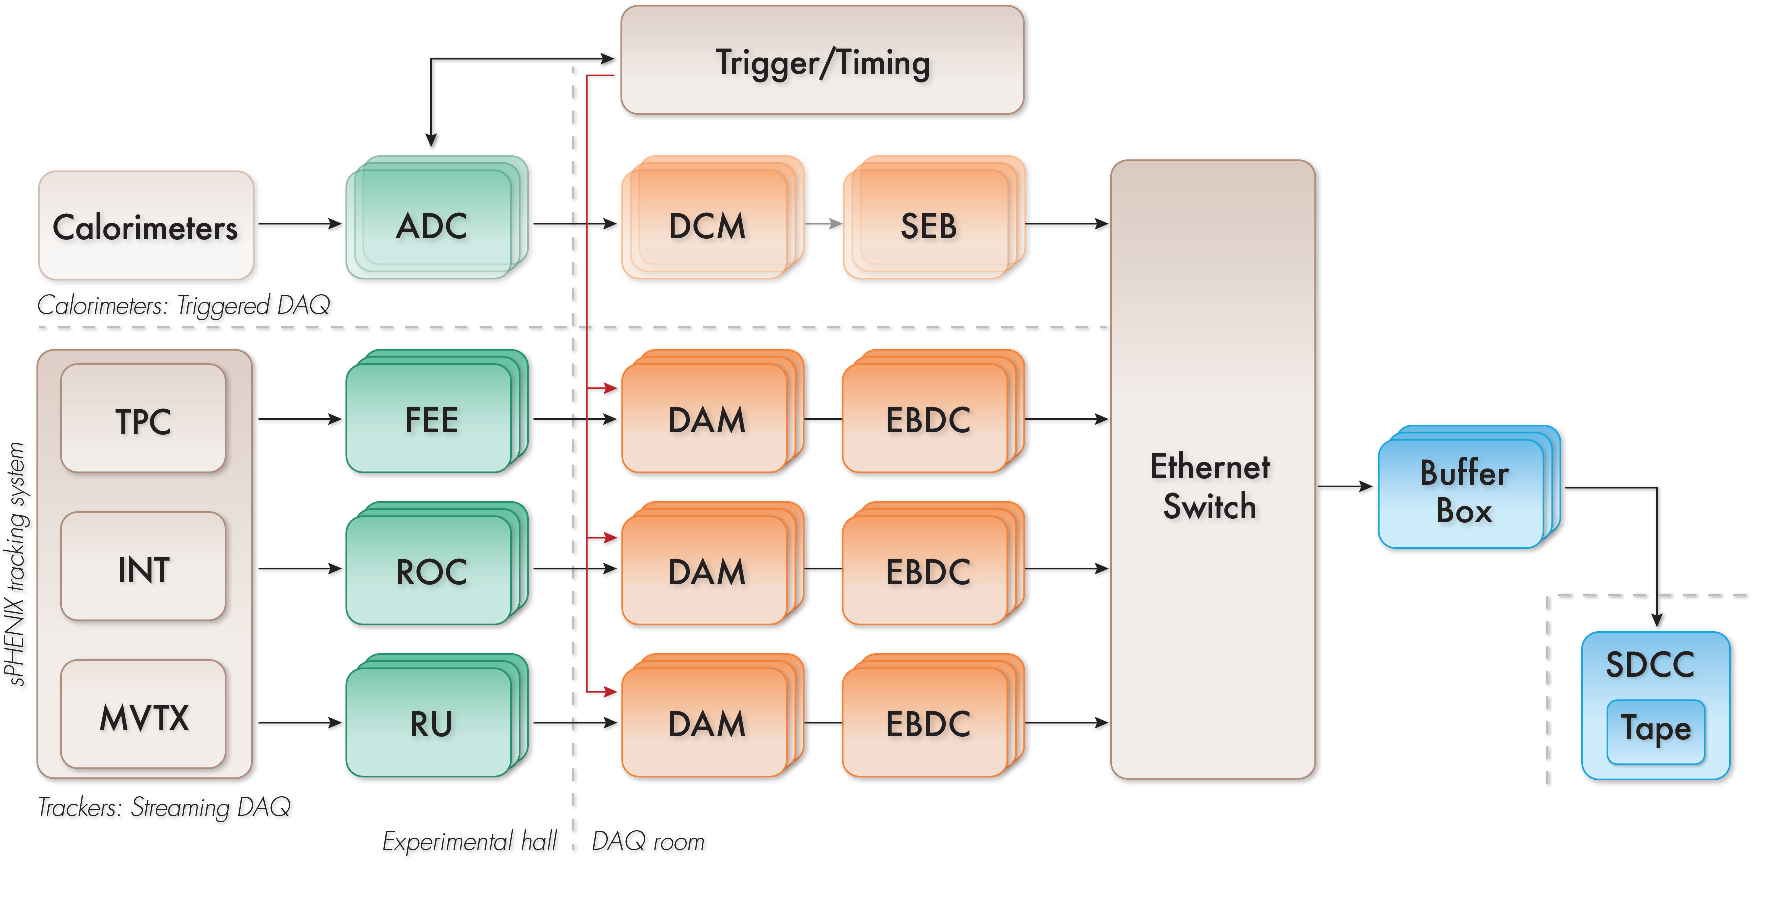
\includegraphics[width=.8\linewidth]{figs/DAQ structure_rev3.pdf}
\caption{The hybrid DAQ structure of the sPHENIX tracking detector, in which  all three tracking detectors are in streaming readout mode. The output of the tracker data stream are throttled to be in synchronize with calorimeter trigger. Additional tracker data can also be streaming to record more minimum bias collisions in addition to the calorimeteric triggered events.}
\label{fig:TPC-DAQ-structure}
\end{center}
\end{figure}
\begin{figure}[htbp]
\begin{center}
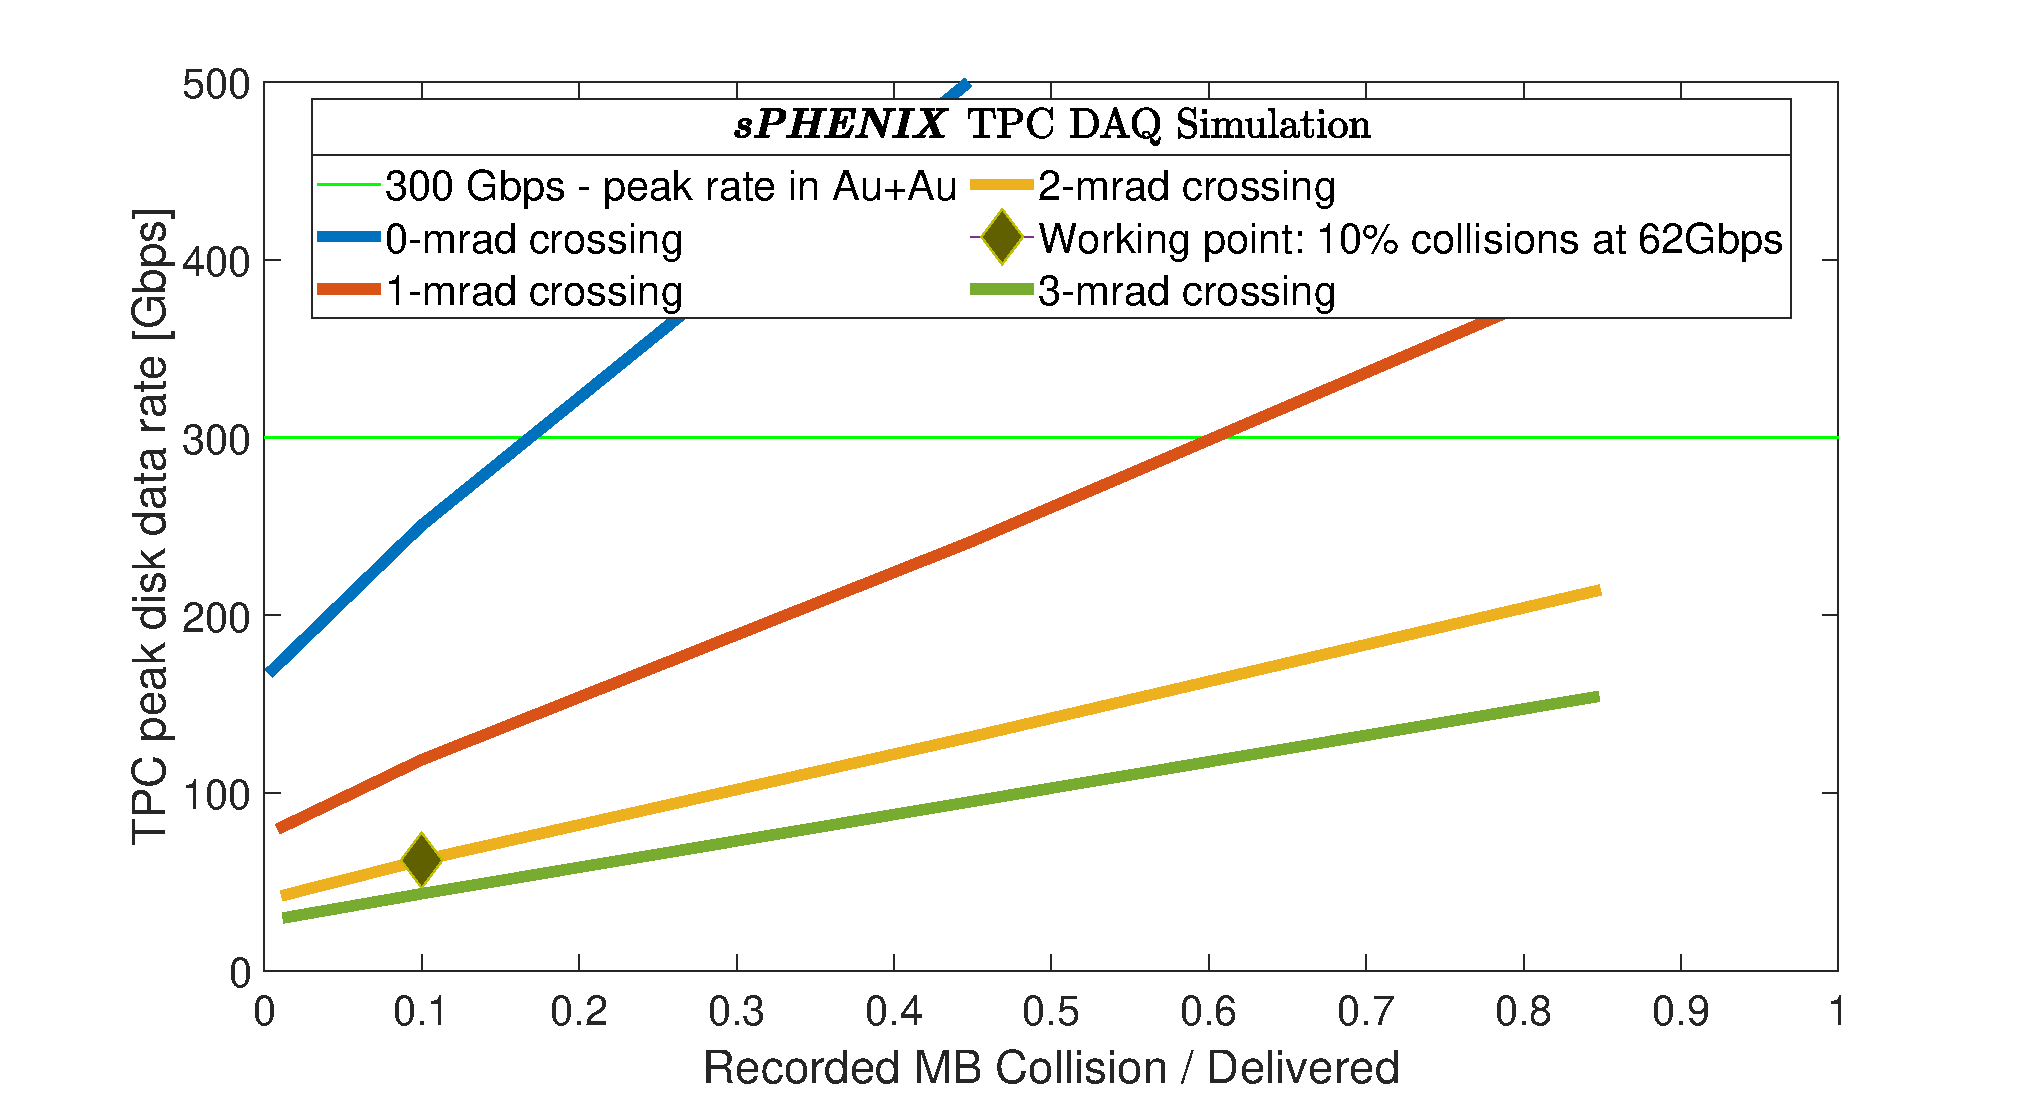
\includegraphics[width=.8\linewidth]{figs/TPCRateLayeredPP_BUP2020_Summary_TriggerWindowRateCoverageCompile.pdf}
% \caption[hoice of operation point between the peak TPC data logging rate and
%   the fraction of M.B. p+p collision recorded.]{\label{fig:TPCRateWindow}
%   Choice of operation point between the peak TPC data logging rate and
%   the fraction of M.B. p+p collision recorded. The green horizontal
%   line denotes the peak data logging rate for Au+Au collisions. At
%   similar logging rate, a minimum of 10\% of \pp M.B. collisions can
%   be streamed to the raw data file as denoted by the solid cyan
%   curve. Other curves denote various online data reduction and beam
%   optimization strategies which would allow recording much higher
%   statistics at a fixed logging rate as further discussed in the last
%   Chapter X.}
\caption{Choice of operation point between the peak TPC data logging rate and the fraction of M.B. p+p collision recorded. The green horizontal line denotes the peak data logging rate for Au+Au collisions. At similar logging rate and without the beam crossing angle, a minimum of 10--20\% of \pp M.B. collisions can be streamed to the raw data file as denoted by the solid blue curve. In the case that a beam cross angle is introduced (red, orange and green curves) the overall data rate can be significantly reduced. The default work point in the 2024 run is with 2~mrad beam crossing angle and record 10\% of collisions at 62 Gbps data rate as denoted by the diamond point.}
\label{fig:TPC-DAQ-rate}
\end{center}
\end{figure}

 
 
\subsection{Hybrid Trigger-Streaming Readout in 2024}
 
In the 2024 run, we plan to implement the first streaming readout DAQ for the tracking detectors to record 10\% of the delivered luminosity in addition to the calorimeteric-triggered events. The data rate and data volume is dominated by the time projection chamber which is studied in Figure~\ref{fig:TPC-DAQ-rate}. With the introduction of the beam crossing angle, the expected data rate with the 10\% streaming readout would be much lower than the design specifications and the previous data volume estimates with zero crossing angle assumed in the 2019 sPHENIX computing plan~\cite{sPH-COMP-2019-001}. The reason is simply because with the 2 milliradian crossing angle there are far fewer collisions outside of $|z|<10$~cm that would have still caused hits in the TPC that would have been recorded.

The physics gain is significant, that includes the \pp reference data for the $D^0$ \raa and the $\Lambda_c/D^0$ ratio both of which are critical for the systematic control in understanding the \AuAu data as discussed in Section~\ref{sec:HF}. In addition, since the \pp beam is transversely polarized, the single spin asymmetry in the $D^0$ channel can be measured to gain access of tri-gluon correlation~\cite{Kang:2008ih, Koike:2011mb}, which is further discussed in Section~\ref{sec:ColdQCD}. 
All aforementioned physics gains would be first measurements at RHIC and uniquely enabled by the streaming DAQ of the sPHENIX trackers.


 
% The upgraded DAQ for the Run2024 \pp and \pA streaming data taking 
% is illustrated in Figure~\ref{fig:TPC-DAQ-structure} and
% summarized in Table~\ref{tab:HFppreach}.  
% The FEE and DAQ hardware of
% each of the three tracking detectors supports a streaming readout mode
% and provides the capability needed for this upgrade. The main work
% will focus on DAQ firmware and software development that enabling the
% streaming capability.  This upgrade would enable the collection of
% sufficient minimum bias in \pp events.  That is, 10\% delivered
% luminosity (see next Chapter) or 200~billion events in the acceptance
% of the vertex tracker, which is a factor of 500 improvement. This
% dataset enables a comprehensive low-$p_T$ hadron program as discussed
% here.  The analysis of these HF hadronic channels does not require
% calorimeter information. Instead, they can be identified with the precision
% tracking detectors of sPHENIX (at $p_T=5$~GeV$/c$, $\sigma(p)/p=1\%$,
% $\sigma(DCA)<10$~$\mu$m ) via a combination of decay topology and
% invariant mass, as demonstrated for even the busiest events of Au+Au
% collisions through detailed simulation studies in~\cite{sPH-HF-2017-002}.

% As summarized in Table~\ref{tab:HFppreach}, an upgraded DAQ for
% sPHENIX trackers will enable the recording of 500 times greater
% statistics of M.B. \pp collisions, which in turn will enable proper HF
% measurements in this key kinematic region.


\subsection{Full streaming Readout for Potential 2026-2027 Running}

In the potential running in 2026 to 2027, we plan to build on the initial experience with streaming readout and aim for stream recording 100\% data stream for the sPHENIX tracking detectors for all collision species. As shown in Figure~\ref{fig:TPC-DAQ-rate}, the data rate would be significantly higher compared the the 2024 work point, but would still be below the bandwidth limit of the readout system. At the expense of higher data volume, full streaming readout of the tracker allows another order of magnitude improvement in the recorded \pp and \pA collision, whose impact is further quantified in Chapter~\ref{chap:beam_use_proposal_extra}.

\subsection{Data Preservation and Data Mining}

This upgrade will accumulate a large amount (10-100\% of delivered luminosity) 
of minimum
bias polarized \pp collision without a trigger bias and with the full
sPHENIX tracking capability and preserved at RHIC computing facility. 
After RHIC completes its scientific
mission at the end of the sPHENIX program, this unique dataset would  allow future data mining for novel quantum effects such as
the quantum coherence in particle productions. 
Such future analysis would have full freedom to define an ``event'' in the offline software ``trigger'' that is based on high level objects such as tracklets and final detector alignment and calibrations. 
These \pp data may be
critical for understanding the future $e+p/A$ collision data at an
Electron Ion Collider~\cite{Accardi2012}.


\section{De-Multiplexing the Calorimeter Readout}
\label{sec:streaming_readout}

\begin{figure}
    \centering
    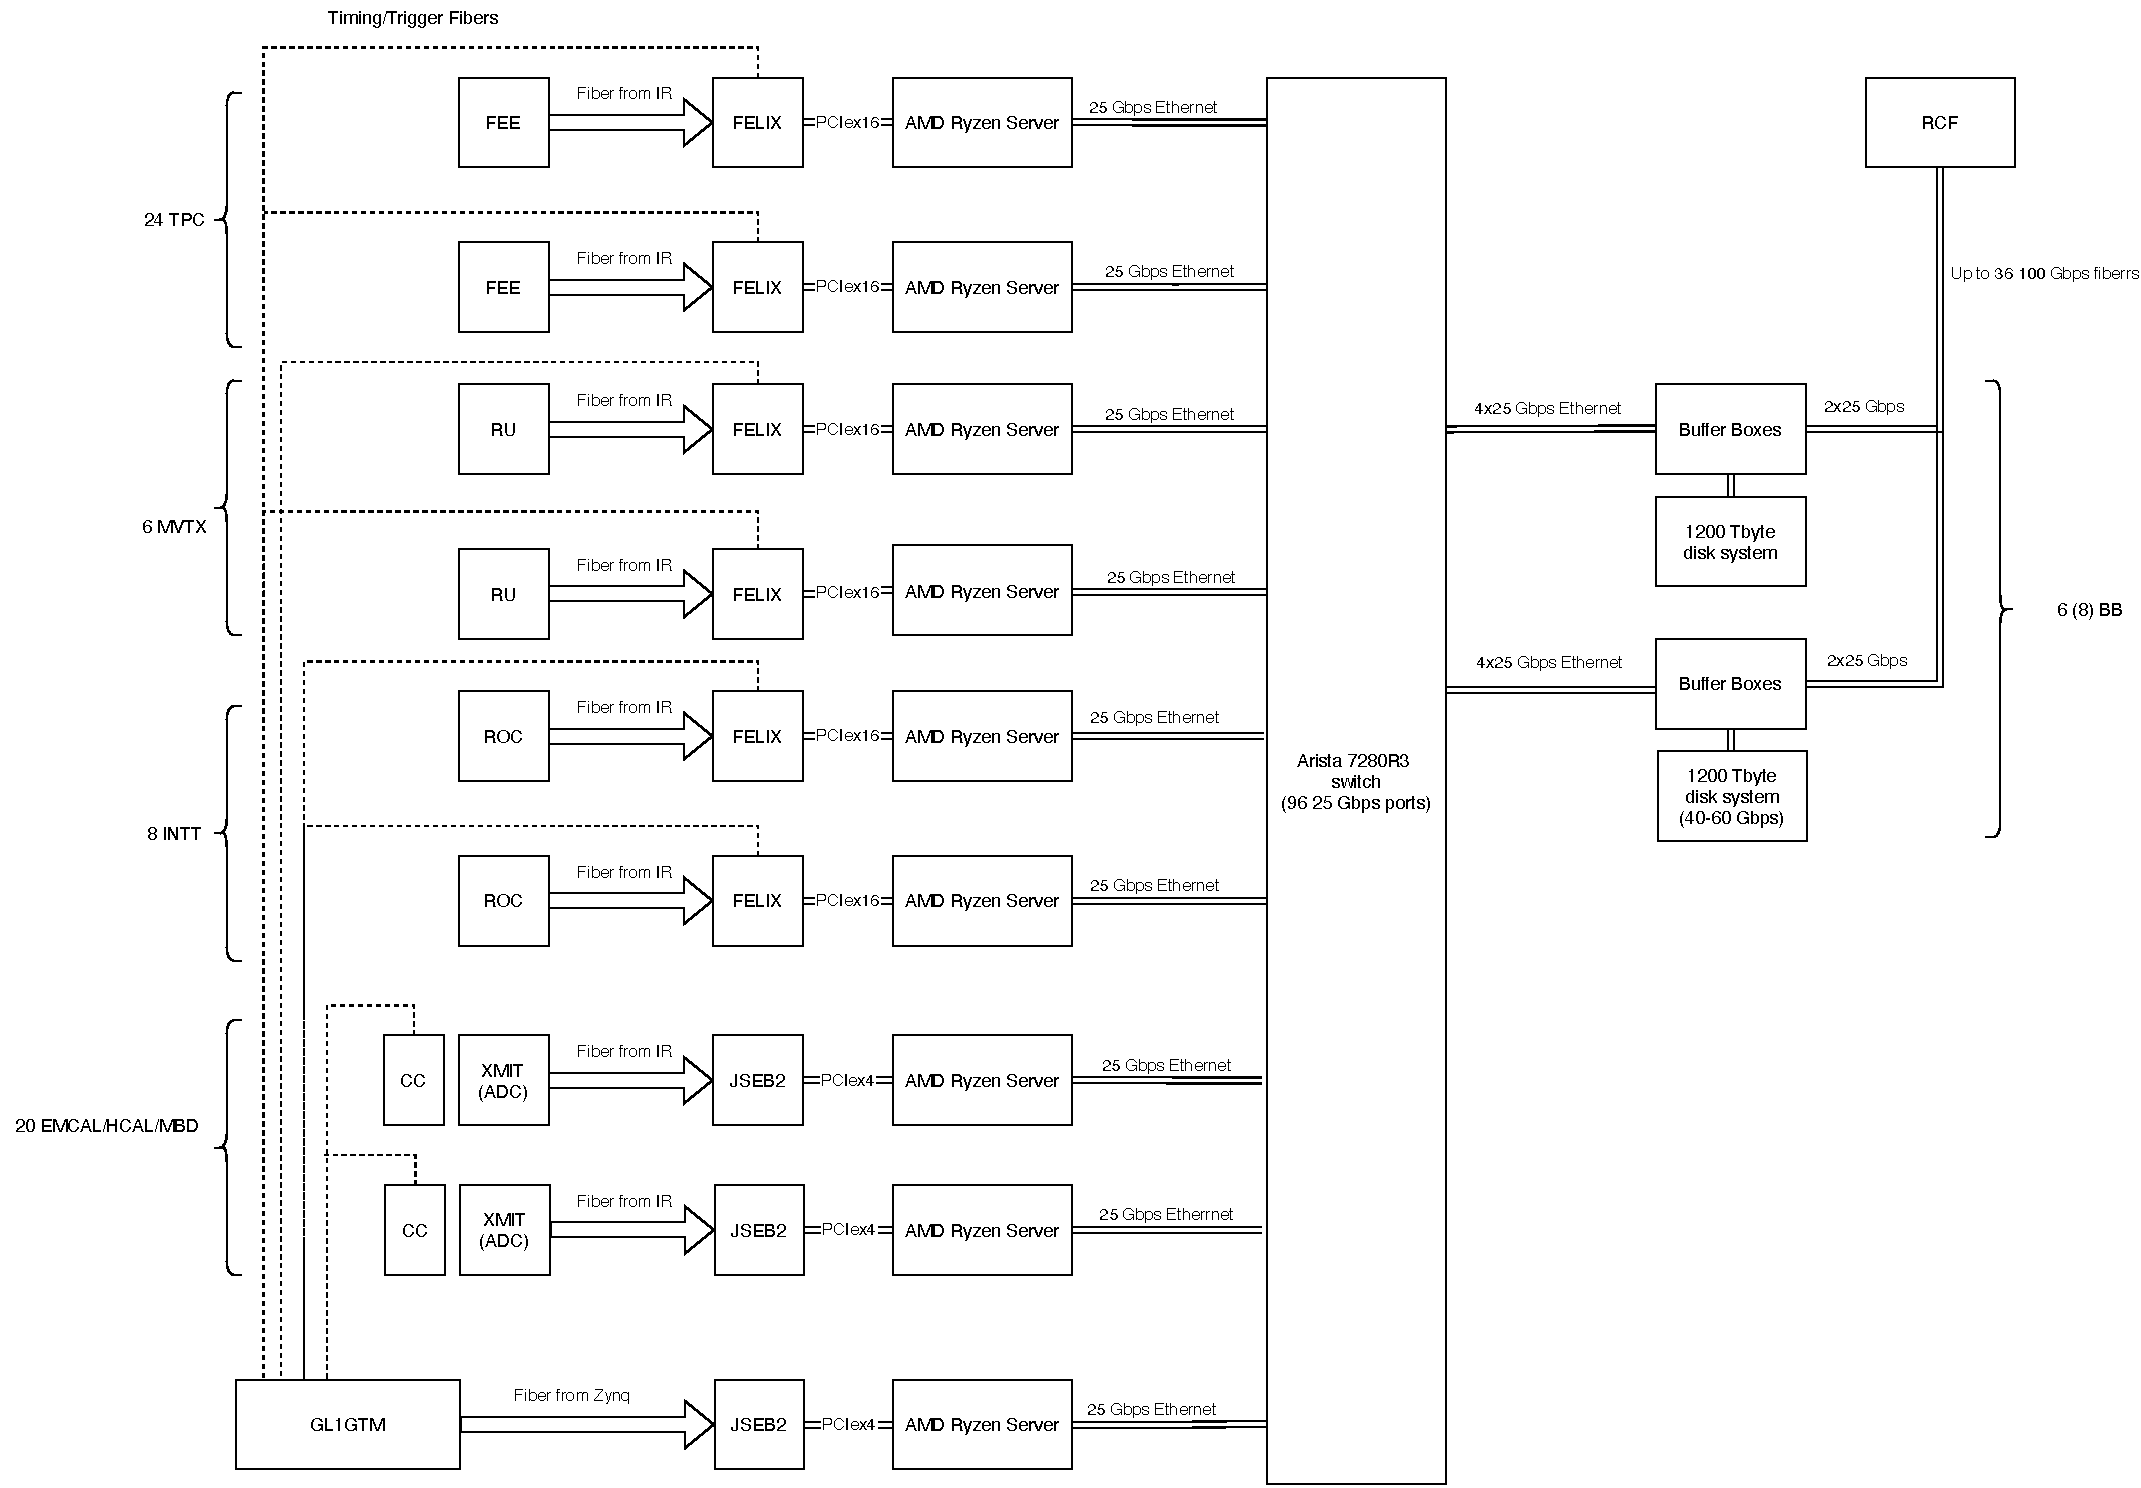
\includegraphics[width=0.85\linewidth]{figs/sphenixdaq_servers_20200803.pdf}
    \caption{Block diagram of sPHENIX data acquisition system, showing
      interfaces to MVTX, INTT, and TPC front end electronics using
      the ATLAS FELIX interface, and electromagnetic and hadronic
      calorimeters and Minimum Bias Detector using the DCM2 and JSEB
      card.} 
    \label{fig:sphenixdaq_servers}
\end{figure}

The sPHENIX data acquisition system is designed to acquire events from
the front end electronics at 15~kHz and a livetime of 90\% or greater.
Custom digitizers on the detector have been designed to transmit data
over fiber optic cables to computers in the sPHENIX Rack Room which
record data to local fileservers before copying the data to the RACF
for archiving and analysis.  A block diagram of the system is shown in
Figure \ref{fig:sphenixdaq_servers}.  The system is designed with high
speed links and buffering at several points to achieve the design
livetime at a 15~kHz event rate.  In the absence of data flow
bottlenecks, the livetime is limited by the ADC system used to read
out the three calorimeters (EMCal, iHCal and oHCal) and the Minimum
Bias Detector.

\begin{figure}
    \centering
    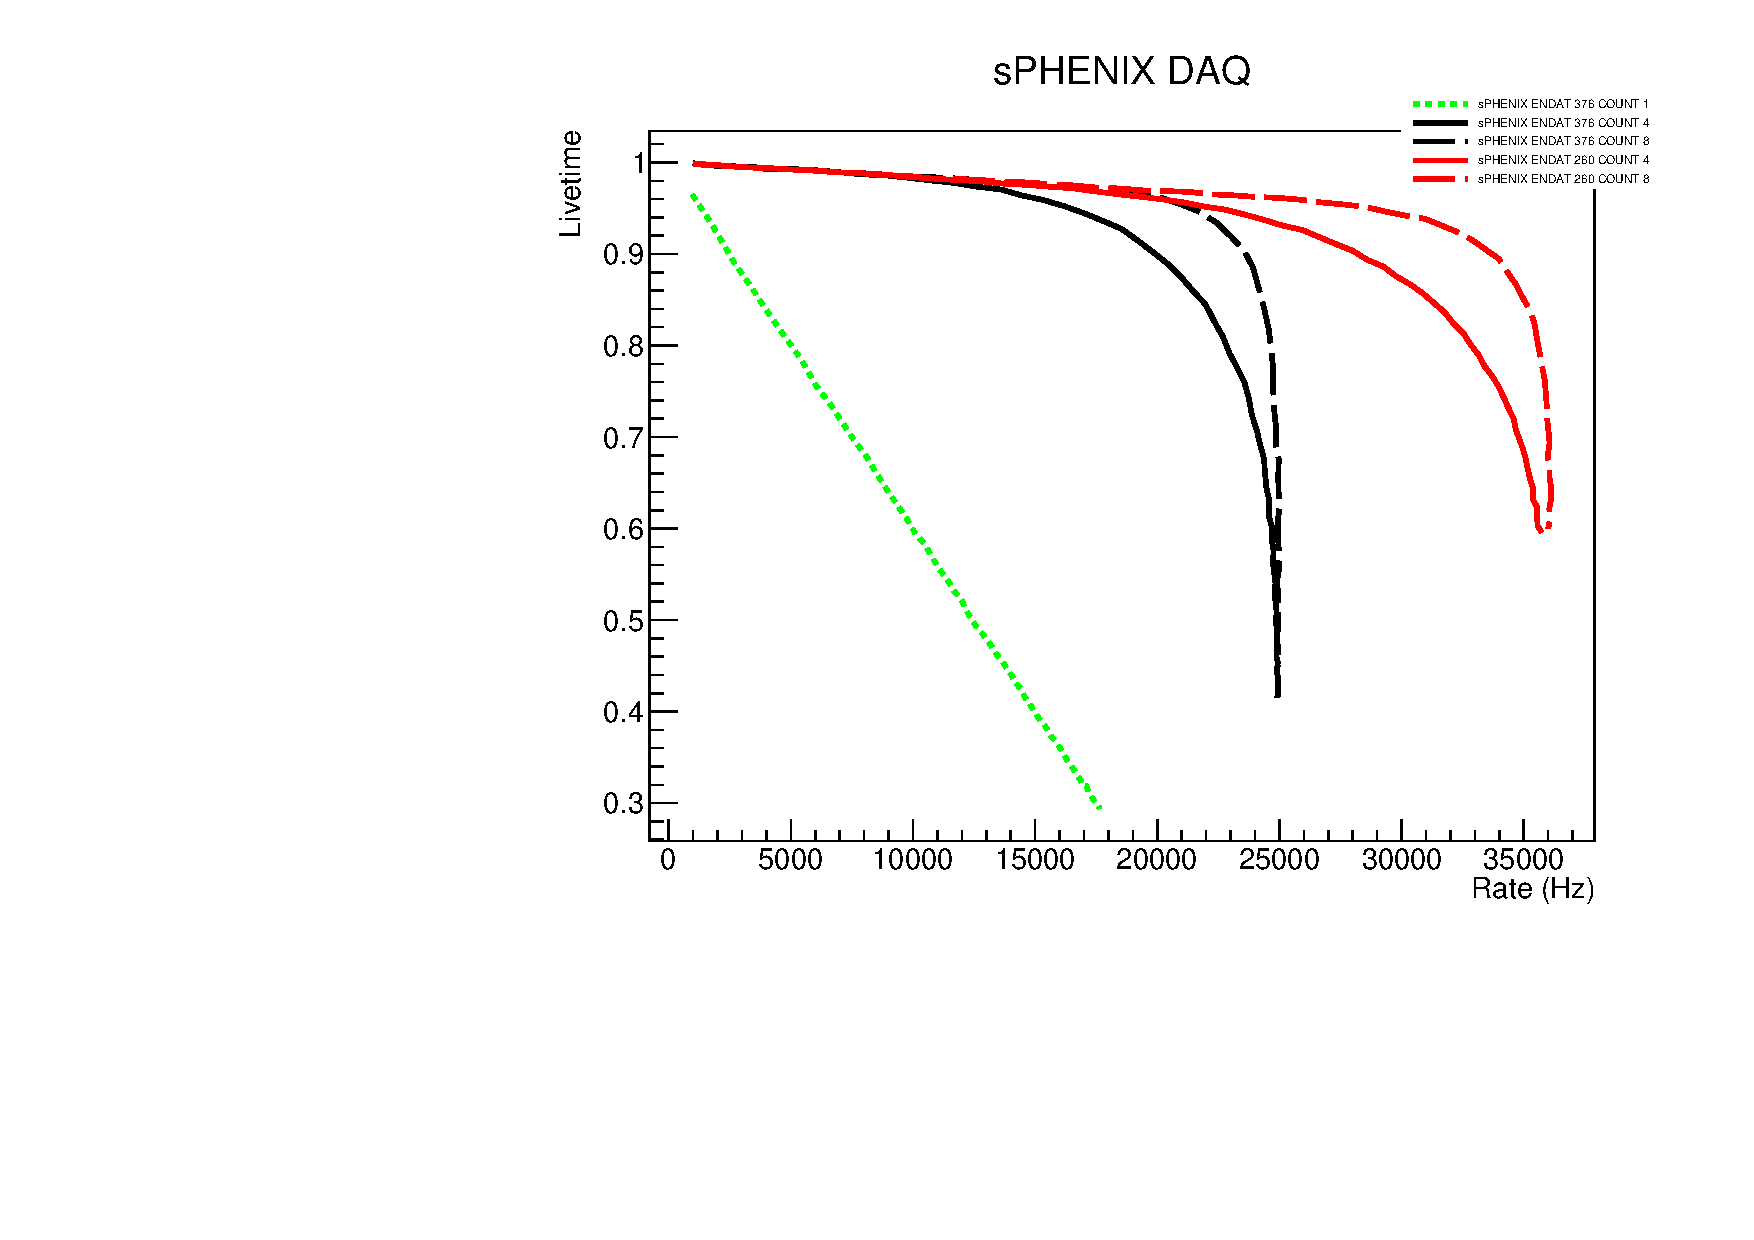
\includegraphics[trim = 0 0 0 25, clip,
    width=0.75\linewidth]{figs/sphenix_daqrate_3.pdf} 
    \caption{Livetime as a function of trigger rate for calorimeter digitizers for
    1, 4, and 8 event buffering in the front end in the baseline design (black),
    and with possible future upgrades (red).  For comparison, the
    green line shows the effect of single event buffering, or
    stop-and-read.} 
    \label{fig:sphenix_daqrate}
\end{figure}

The ADC system used by the calorimeters uses 60~MHz waveform
digitizers to record a fixed number of samples at the time of a
Level-1 trigger, which are buffered locally on the detector for 4, and
possibly as many as 8, events before serialization and transmission
over optical fiber from a digitizer "XMIT" board to second generation
Data Collection Modules (DCM II) --- reused from the PHENIX experiment
--- which zero suppress and re-format the data.  The sPHENIX baseline
design collects data from three ADC modules (192 channels) to one
fiber (by way of the XMIT board), and the time to transmit an event
ultimately determines the livetime as a function of event rate.
Assuming there are no data transmission bottlenecks downstream which
would require throttling the data flow, the transmission time for a
single event is designed to be about 40~$\mu$sec.  Buffering events at
the digitizer makes it possible to achieve a livetime greater than
90\% with 15~kHz of input triggers, but the livetime decreases as the
trigger rate approaches 25~kHz, as shown by the black curves in Figure
\ref{fig:sphenix_daqrate}.

A possible upgrade to the ADC system which could nearly double the
rate of recorded events while maintaining the 90\% livetime would be
to decrease the number ADC modules serialized on one fiber in the
electromagnetic calorimeter.  Reducing the number of ADC boards per
fiber to two would not require more crates on the detector, and would
decrease the transmission time to about 28~$\mu$sec, as shown by the
red curves in Figure \ref{fig:sphenix_daqrate}.

This upgrade would require 64 additional XMIT boards and eight
additional DCM II boards as well as some additional electronics, fibers,
and crates to serve them.  A rough estimate of the cost is
\$100k-\$150k in electronics and a similar cost for engineering, for a
total cost of about \$300k.  Due to parts obsolescence and continuing
advances in electronics, it could be preferable to design a
replacement for the DCM II modules, but it is not practical to consider such a
project until the baseline electronics is installed and operating.

%%%



\chapter{Physics Projections 2023-2025}
\label{chap:physics_projections}

In this Chapter we present a sampling of the key physics that sPHENIX will deliver with the run plan for 2023-2025 detailed in Chapter~\ref{chap:beam_use_proposal}.    We highlight that the project uncertainties shown in the following sections are under the 28 cryo-week scenarios and easily scaled to the 24 cryo-week scenarios.  In the case of nuclear modification factors, the results include uncertainties in the numerator from the A+A running and the denominator from the p+p reference data sets.

\section{Jet and Photon Physics}
\label{sec:jet}

Probing the Quark-Gluon Plasma with precise jet, direct photon, and hadron measurements is a core aspect of the sPHENIX scientific program. Between 2023 and 2025, sPHENIX will collect high statistics data samples to allow for detailed reconstructed jet measurements, including jet yields, di-jet events, jet (sub-)structure and properties, photon-tagged jet quenching measurements, and jet-hadron correlations. As a note, the projections in this Section are for light flavor jets, and statistical projections for $b$-quark jet yields and their properties are discussed below in Sec.~\ref{sec:HF}. 

To form the projections in this section, the perturbative QCD calculations previously used in the sPHENIX MIE proposal document~\ref{Adare:2015kwa} were applied to the nominal running plan proposed in Sec.~\ref{chap:beam_use_proposal}. 
For $p$+$p$ collision, it is assumed that all photons and jets can be efficiently selected by a calorimeter trigger above a moderate $p_\mathrm{T}$ value, and that high-$p_\mathrm{T}$ charged hadrons can be selected indirectly via a jet trigger. For Au+Au collisions, it is assumed that jets and charged hadrons will only be measured in Minimum Bias events, but that the statistics for high-$p_\mathrm{T}$ photons can be populated by a photon trigger in Au+Au data-taking.

Fig.~\ref{fig:jet_RAA_proj} (left) shows the projected total yield of jets, direct photons, and hadrons in $p$+$p$ collisions and in 0--20\% central Au+Au collisions, using a Glauber MC simulation~\cite{Miller:2007ri} to translate a Au+Au event yield to a hard process yield. Overall suppression factors of $R_\mathrm{AA} = 0.2$, $0.4$ and $1.0$ are assumed for hadrons, jets, and photons in central Au+Au events. 

As another way of indicating 

Statistical projections for the nuclear modification  yields of reconstructed jets, photons, and charged hadrons are expressed in Fig.~\ref{fig:jet_RAA_proj} 

\section{Upsilon Physics}
\label{sec:upsilon}

High statistics measurements of the Upsilon states with sufficient precision for clear separate of said states $\Upsilon(1s,2s,3s)$ is one of the key deliverables of the sPHENIX physics program.  Shown in Figure~\ref{fig:upsilon3years} are the projected statistical uncertainties for the $\Upsilon(1s)$ and $\Upsilon(2s)$ states as a function of $p_{T}$ in 0-10\% central Au+Au collisions.   We note that the $\Upsilon(3s)$ is so far not observed in Pb+Pb collisions at the Large Hadron Collider, and so might only result in an upper limit from sPHENIX depending on the yields.   

Also, shown are results for the three-states assuming a particular model (!) for the nuclear modification factor as a function of centrality.   NEED FIGURE FROM TONY!

\begin{figure}
    \centering
    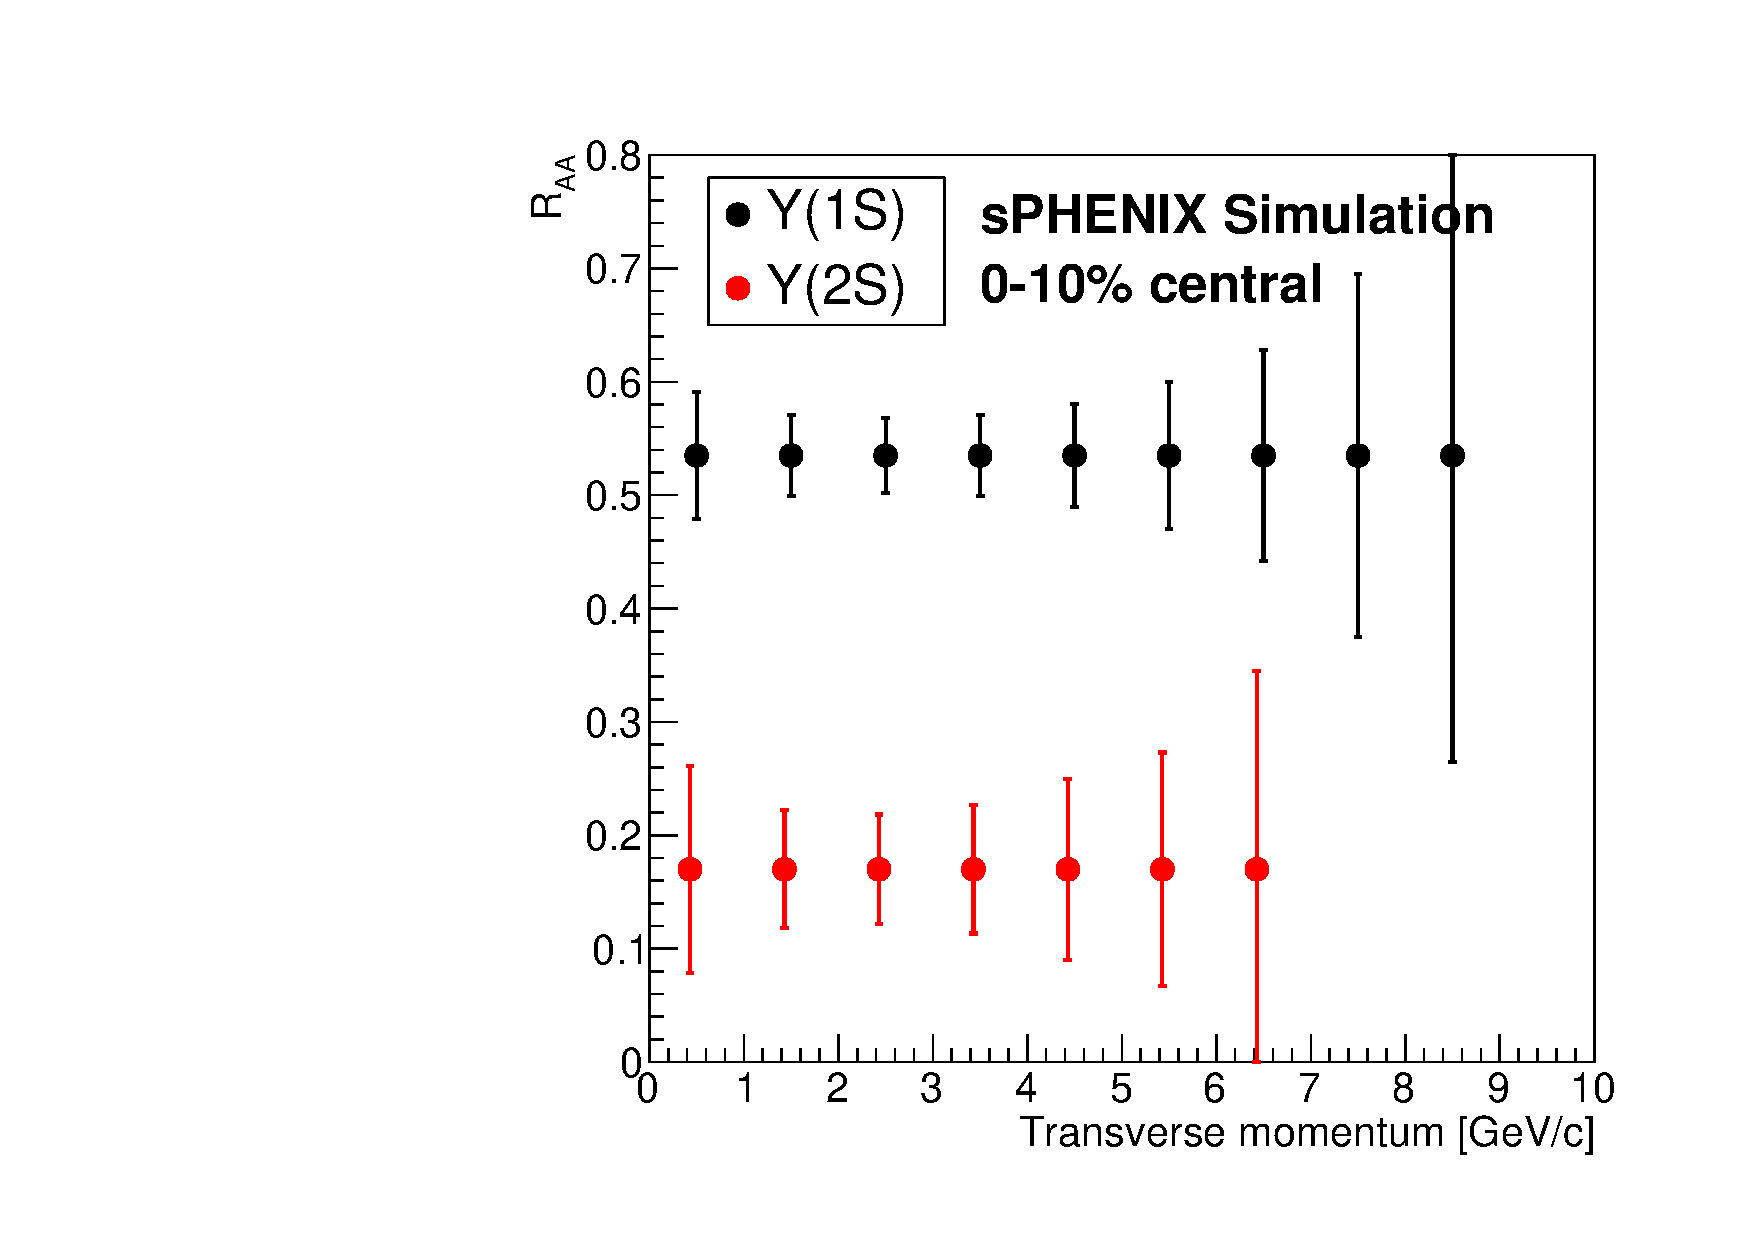
\includegraphics[width=0.55\linewidth]{figs/BUP_Upsilon_RAA_3yr_28wks.pdf}
    \caption{{\textcolor{red}{PLACEHOLDER FIGURE FROM TONY FRAWLEY}}. sPHENIX projected statistical uncertainties, including from background subtraction contributions, for the Upsilon nuclear modification factors from the three-year (2023-2025) proposed run plan.   The projections are assuming the 28 cryo-weeks in each year.
    \label{fig:upsilon3years}}
\end{figure}

\section{Open Heavy Flavor Physics}
\label{sec:HF}

(intro)

\subsection{Diffusion and energy loss of Heavy Quarks in the QGP}


\begin{figure}[htbp]
\centering
% 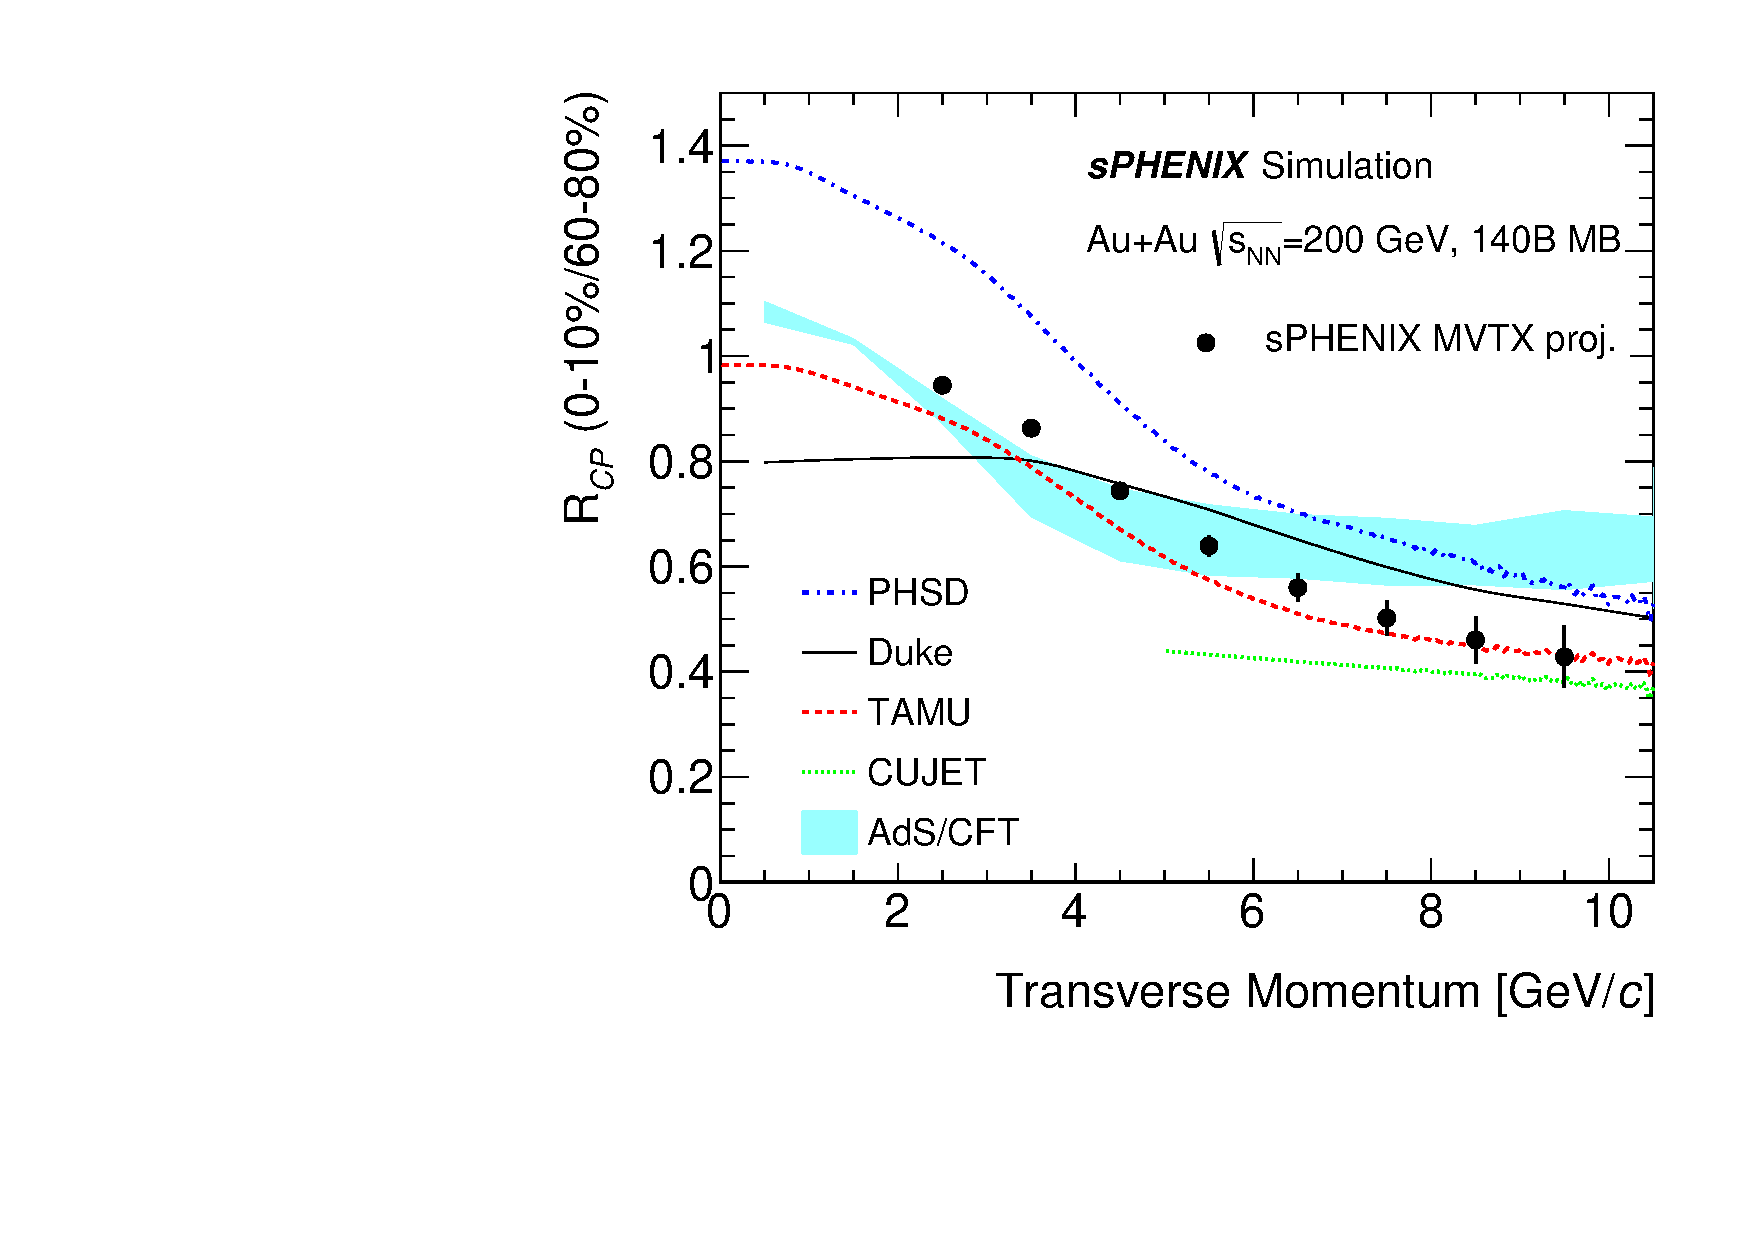
\includegraphics[width=0.48\textwidth]{figs/Rcp_proj_140B_theory.pdf}
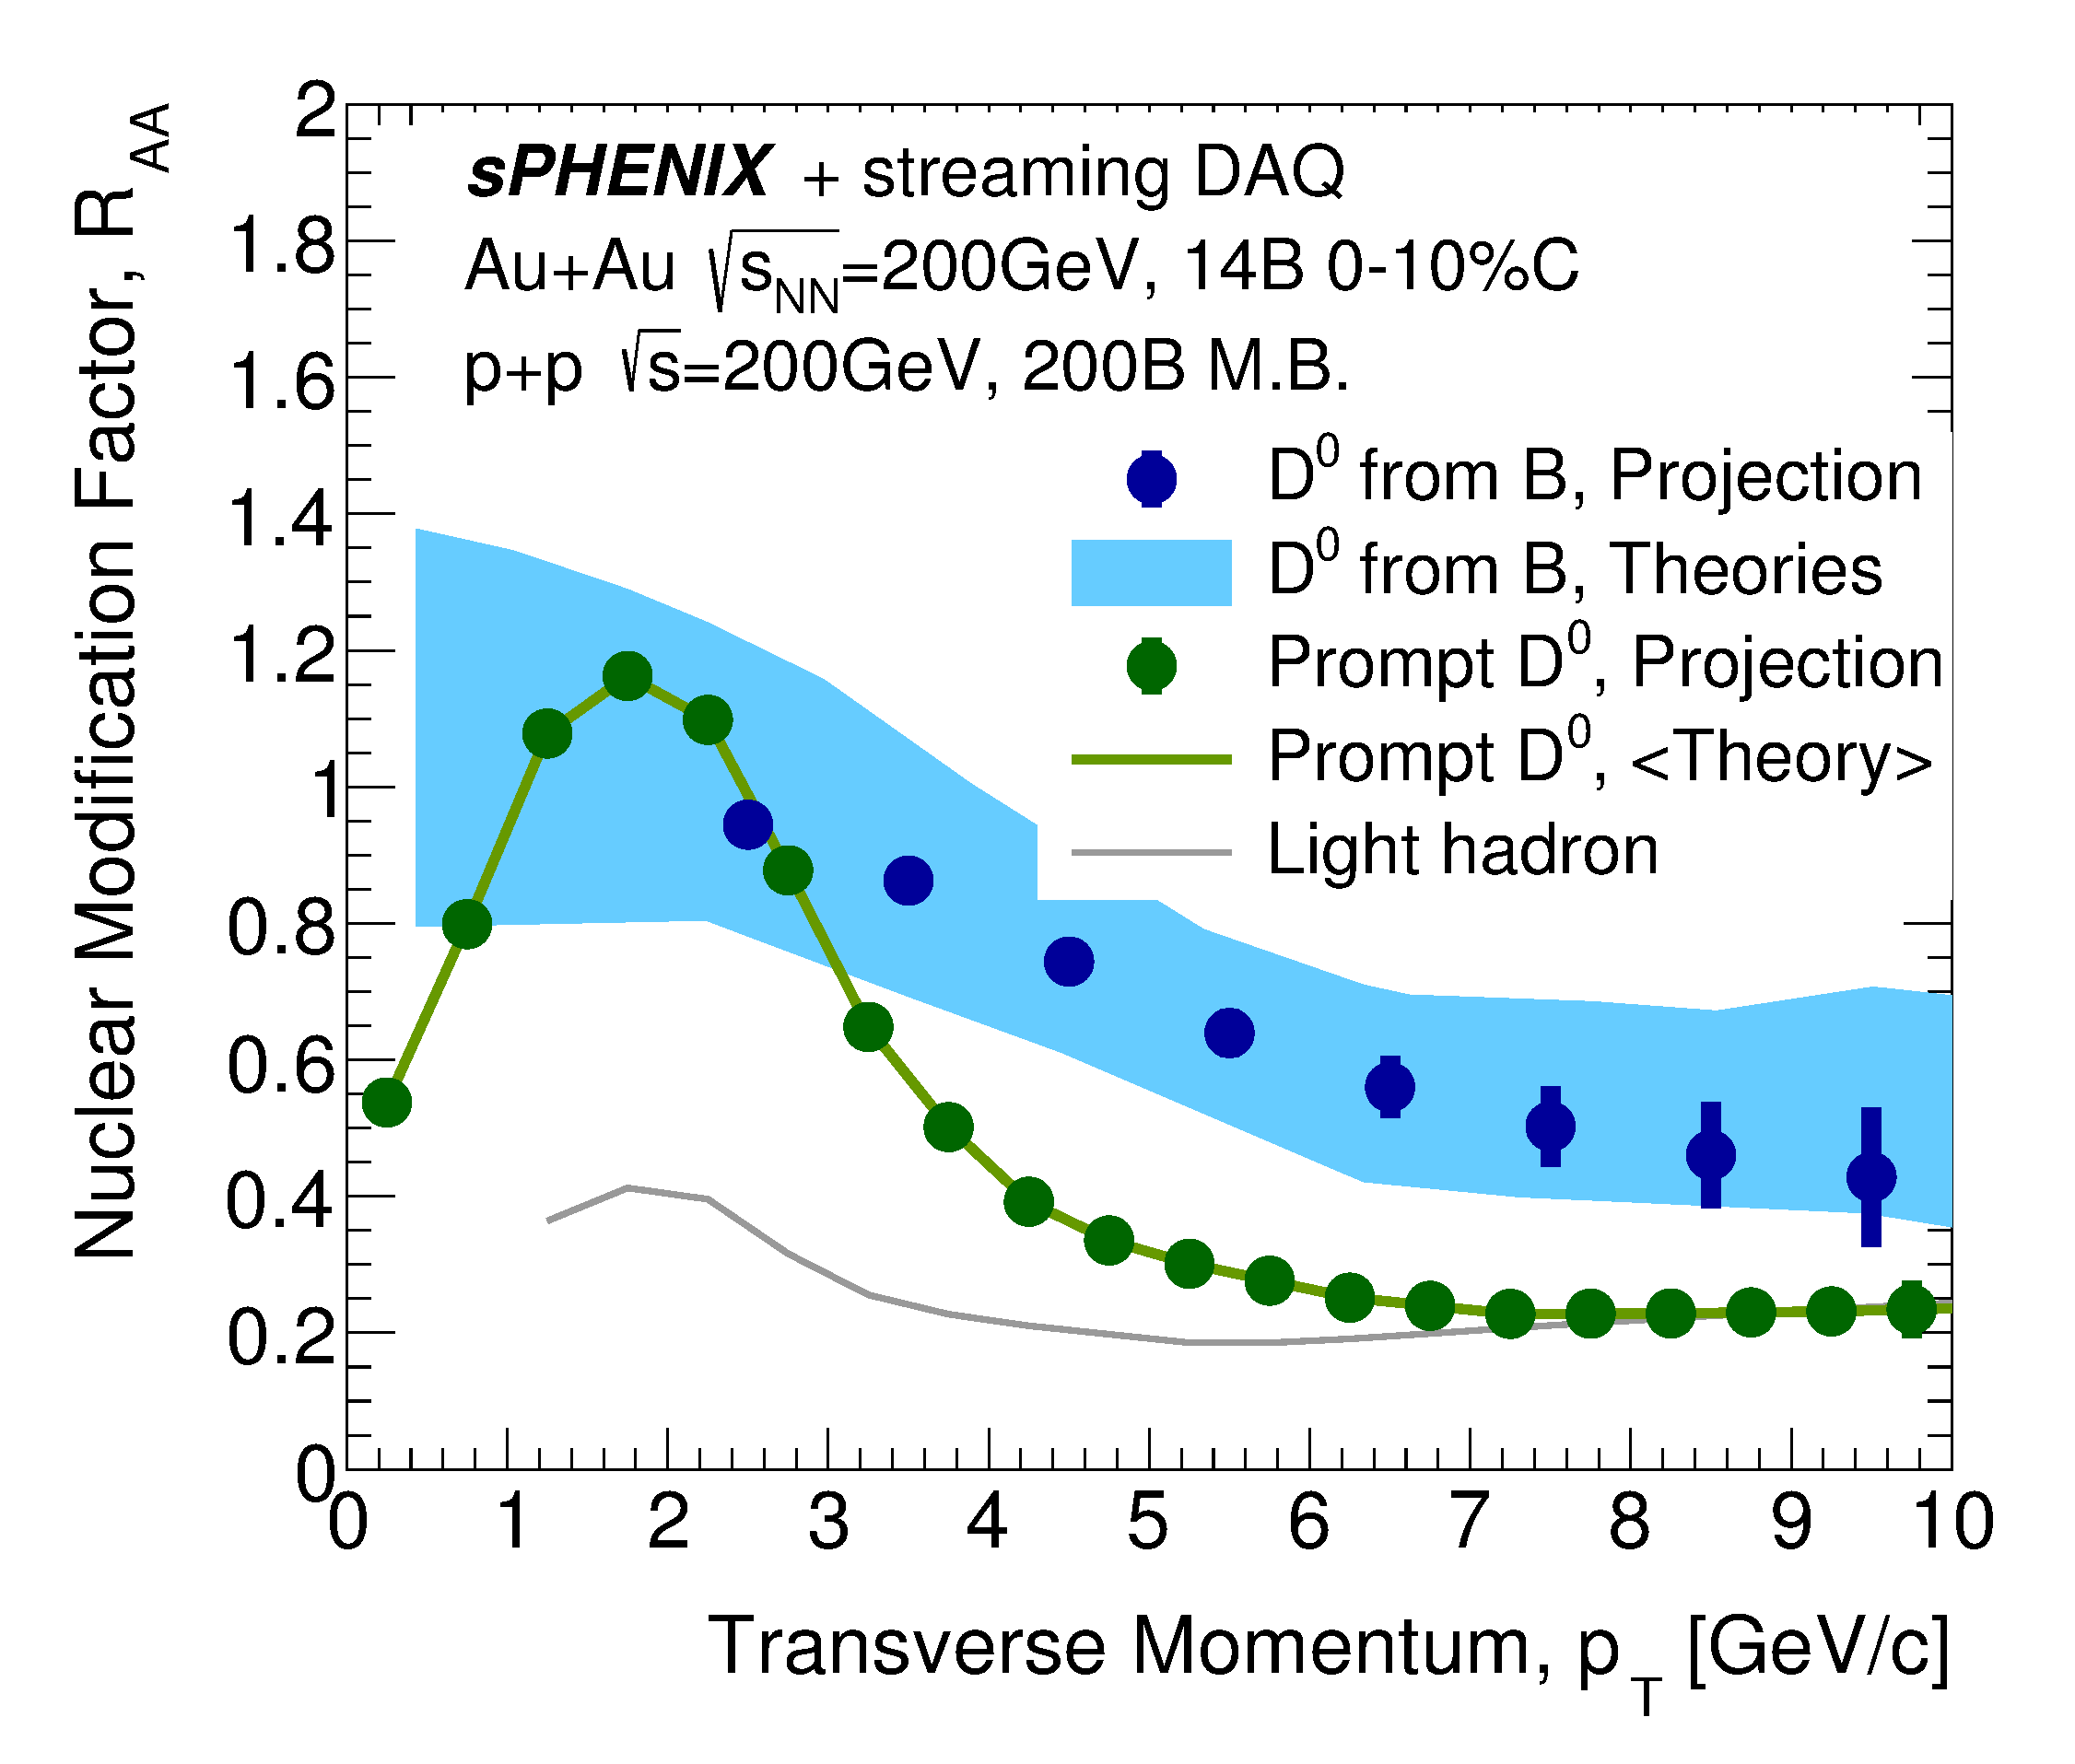
\includegraphics[width=.49\linewidth]{figs/RAA_DB_theory_root_RAADB_pp200B.pdf}
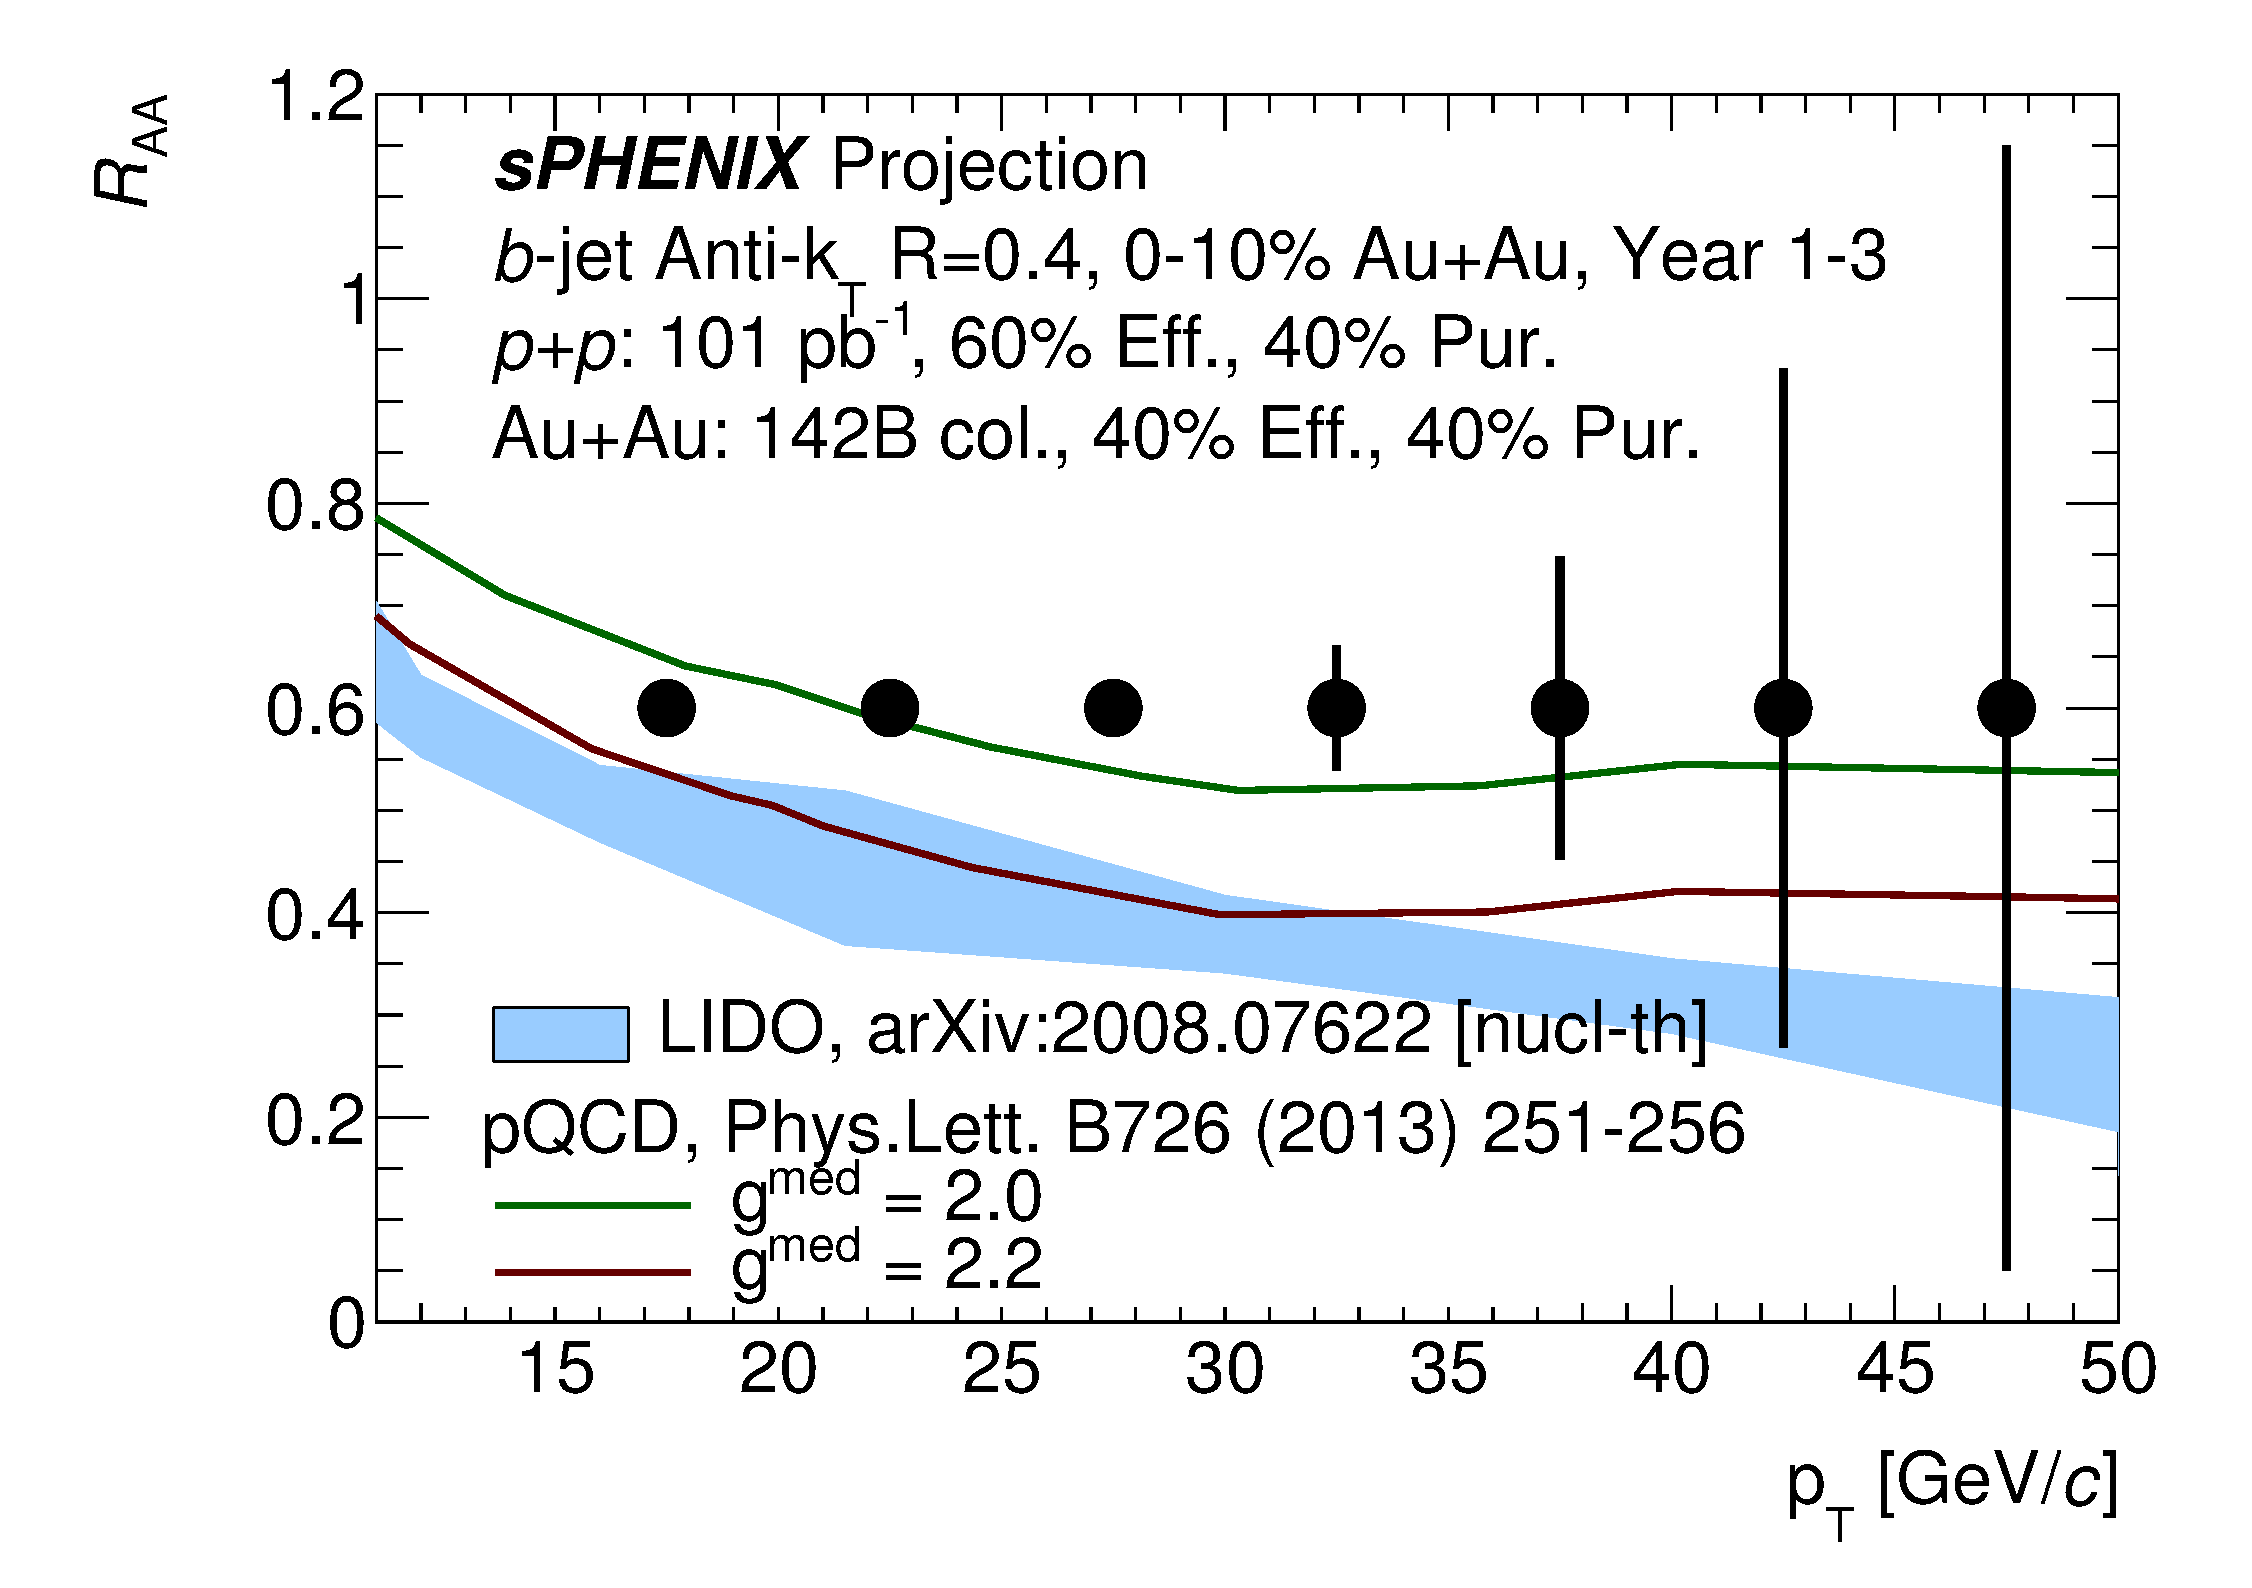
\includegraphics[width=0.5\textwidth]{figs/200pp_pythia8_CTEQ6L_7GeV_ALL_cfg_eneg_DSTReader_root_Draw_HFJetTruth_CrossSection2RAA_Theory_3yr_deta0_70.pdf}
\caption{Projected statistical uncertainties of nuclear modification factor $R_{cp}$ and \raa measurements of non-prompt/prompt $D^0$ mesons (left) and $b$-jet (right) as a function of \pT in 0--10\% central \auau collisions at $\sqrt{s_{NN}}=200$~GeV from a dataset of 140 billion minimum bias \auau collisions expected from the three-year sPHENIX operation. Left: the solid blue and red lines are best fit to the RHIC data, the solid black line is from a model calculation for B mesons and the dotted line is the theory calculation for $D$-mesons coming from $B$-meson decays. Right: the solid and dashed lines are from model calculations with two different coupling parameters to the QGP medium, $g^{\textrm{med}}$, and the statistical projection is based on the assumption of $\raa =0.6$. sPHENIX will enable these highest precision $B$-meson measurement and the first heavy flavor jet measurement at RHIC, which will place stringent tests on models describing the coupling between heavy quarks and the QGP~\cite{Huang:2013vaa,Duke,TAMU,PHSD,CUJET}}
\label{fig:HF-inclusive-RAA}
\end{figure}

\begin{figure}[htbp]
\centering
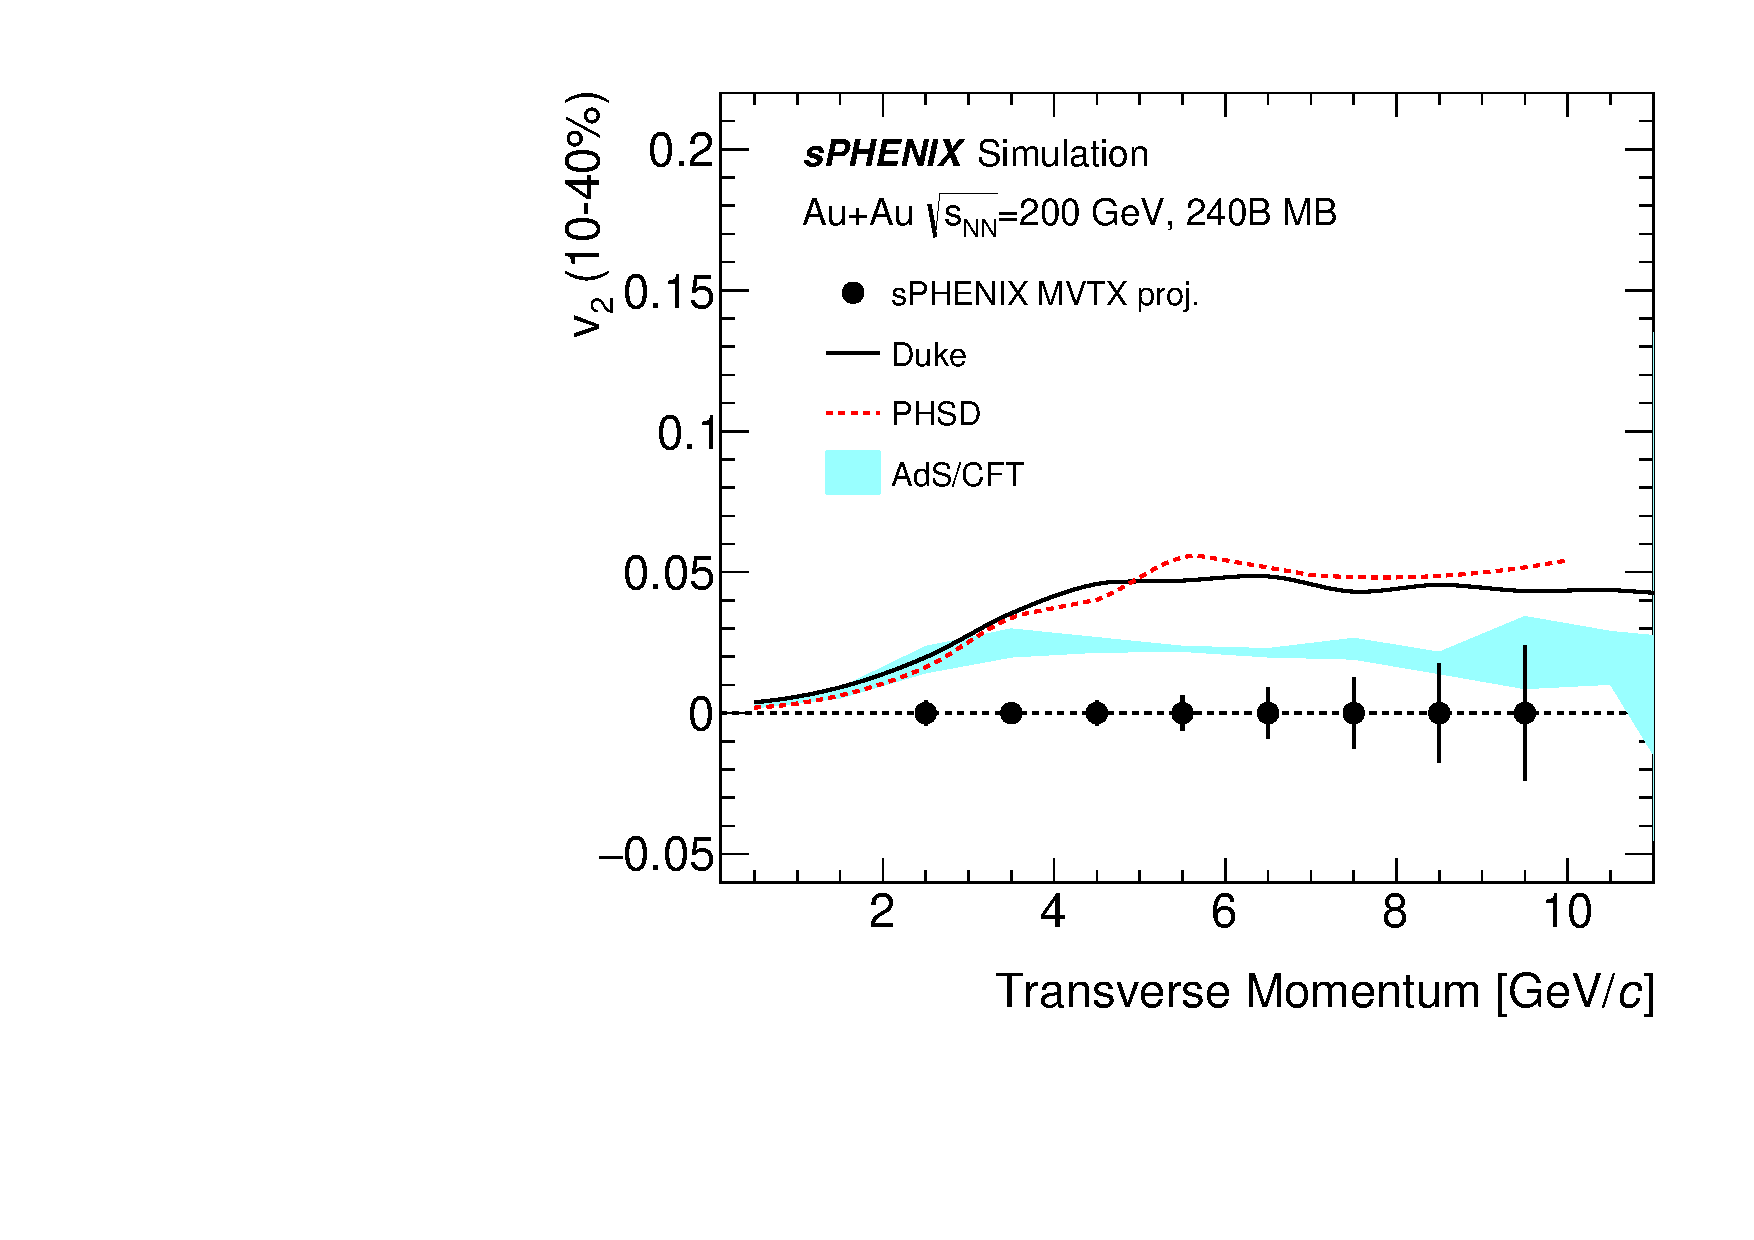
\includegraphics[width=0.48\textwidth]{figs/v2_proj_240B_theory.pdf}
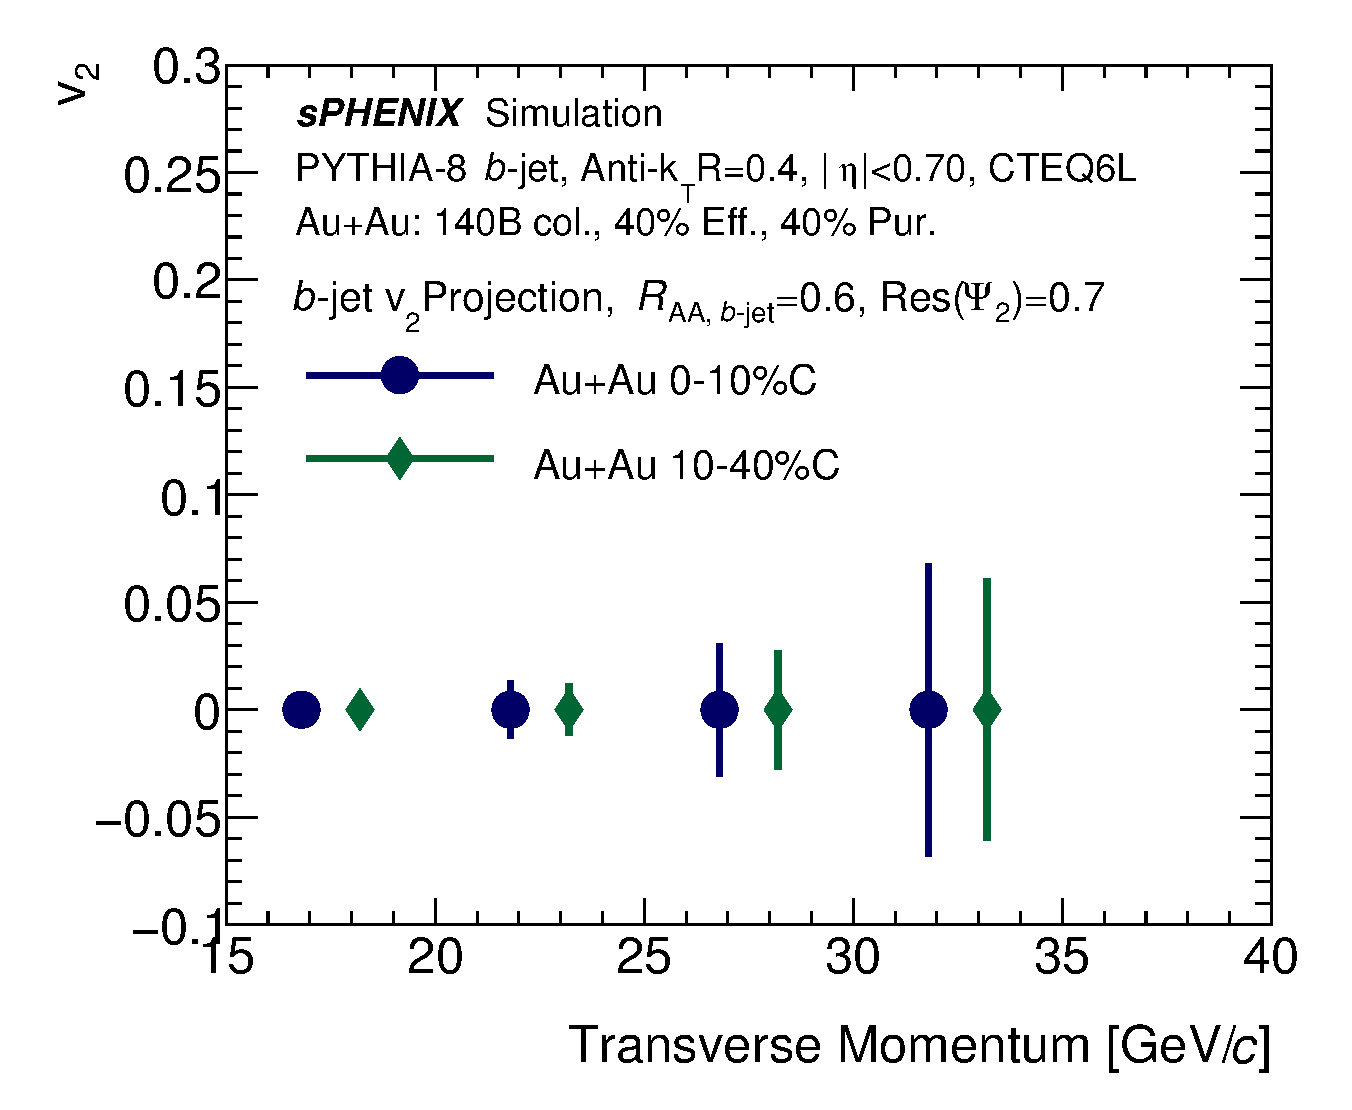
\includegraphics[width=0.5\textwidth]{figs/200pp_pythia8_CTEQ6L_7GeV_ALL_cfg_eneg_DSTReader_root_Draw_HFJetTruth_CrossSection2v2_3yr_EPR0_7_deta0_70.pdf}
\caption{Projected statistical uncertainties of $v_2$ measurements of non-prompt/prompt $D^0$ mesons (left) and $b$-jets (right) as a function of \pT in 10--40\% central \auau collisions at $\sqrt{s_{NN}}=200$~GeV from a dataset of 140 billion minimum bias \auau events expected from the three-year sPHENIX operation.  Left: the blue dotted line is from best fit of RHIC data, and the black line is for $B$-meson assuming $m_T$ scaling in $v_2$. \cite{Adamczyk:2017xur, Duke, TAMU, PHSD}}
\label{fig:HF-v2}
\end{figure}


\begin{figure}[htbp]
\centering
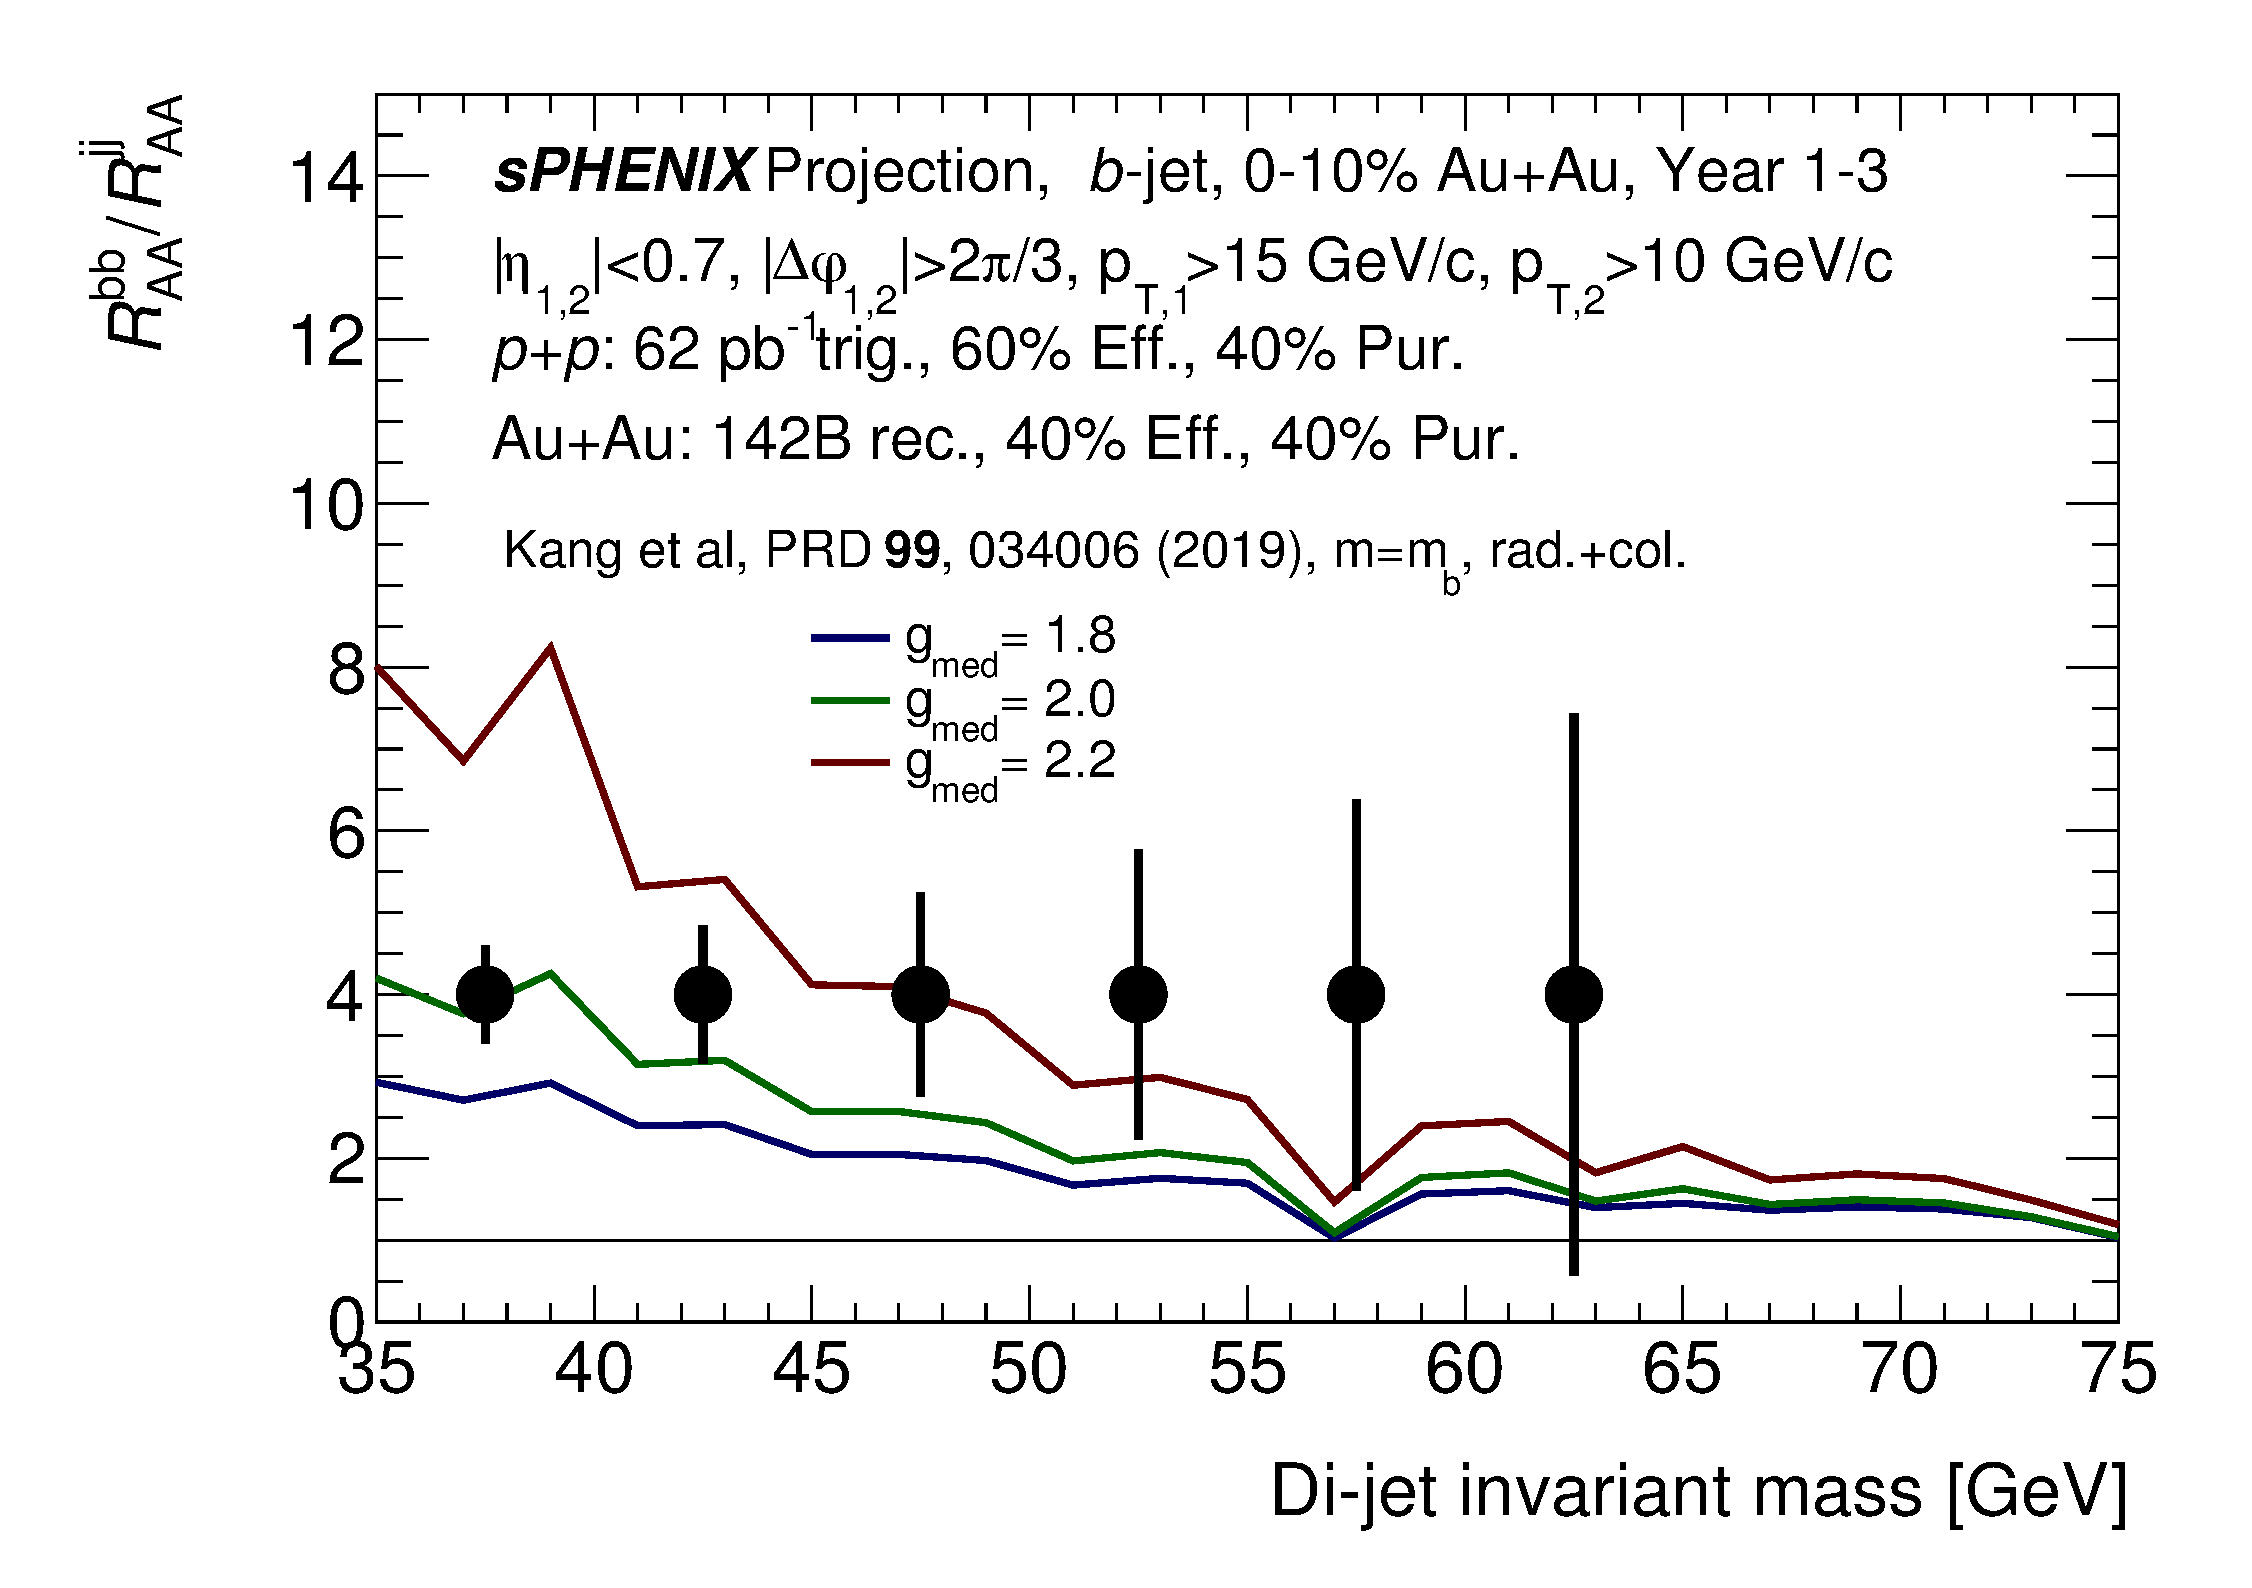
\includegraphics[width=0.48\textwidth]{figs/200pp_pythia8_CTEQ6L_7GeV_ALL_cfg_eneg_DSTReader_root_Draw_HFJetTruth_InvMass_CrossSection2RAARatio_Theory_3yr_deta0_70.pdf}
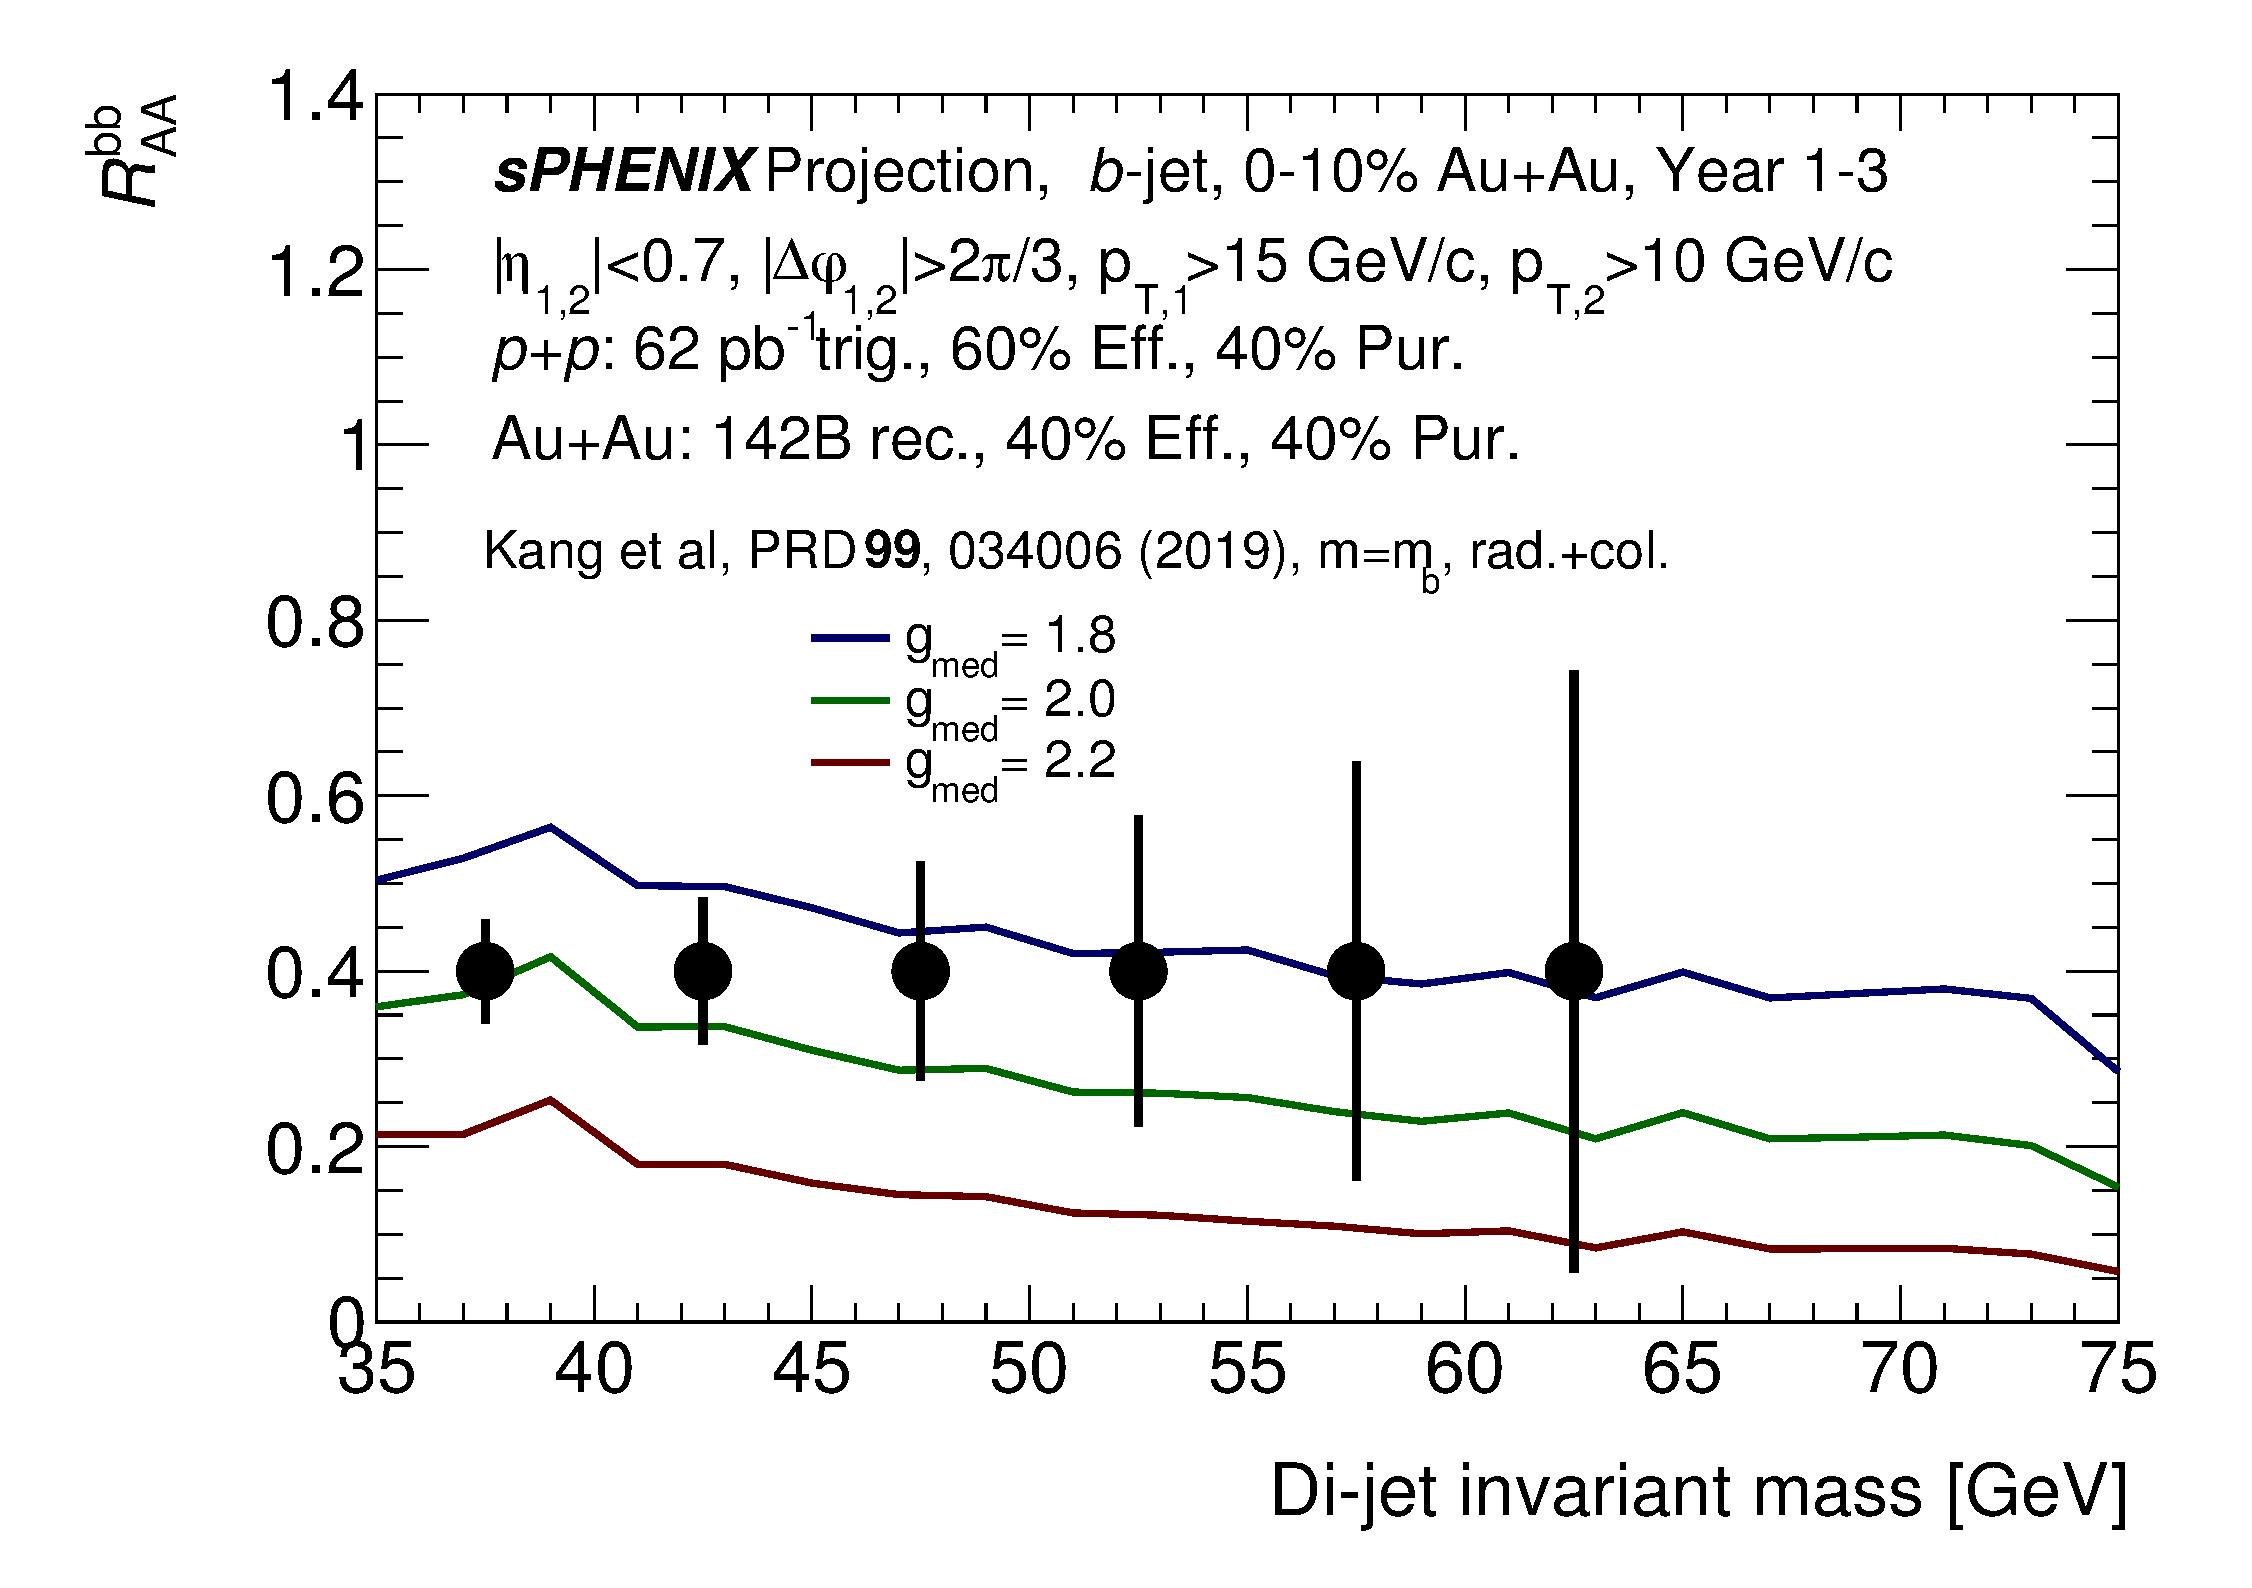
\includegraphics[width=0.5\textwidth]{figs/200pp_pythia8_CTEQ6L_7GeV_ALL_cfg_eneg_DSTReader_root_Draw_HFJetTruth_InvMass_CrossSection2RAA_Theory_3yr_deta0_70.pdf}
\caption{Projected statistical uncertainties of nuclear modification for $b$-jet pairs and $b$-jet-light-jet super-ratio.}
\label{fig:HF-bjet-pair}
\end{figure}


% \begin{figure}[htbp]
% \begin{center}
% 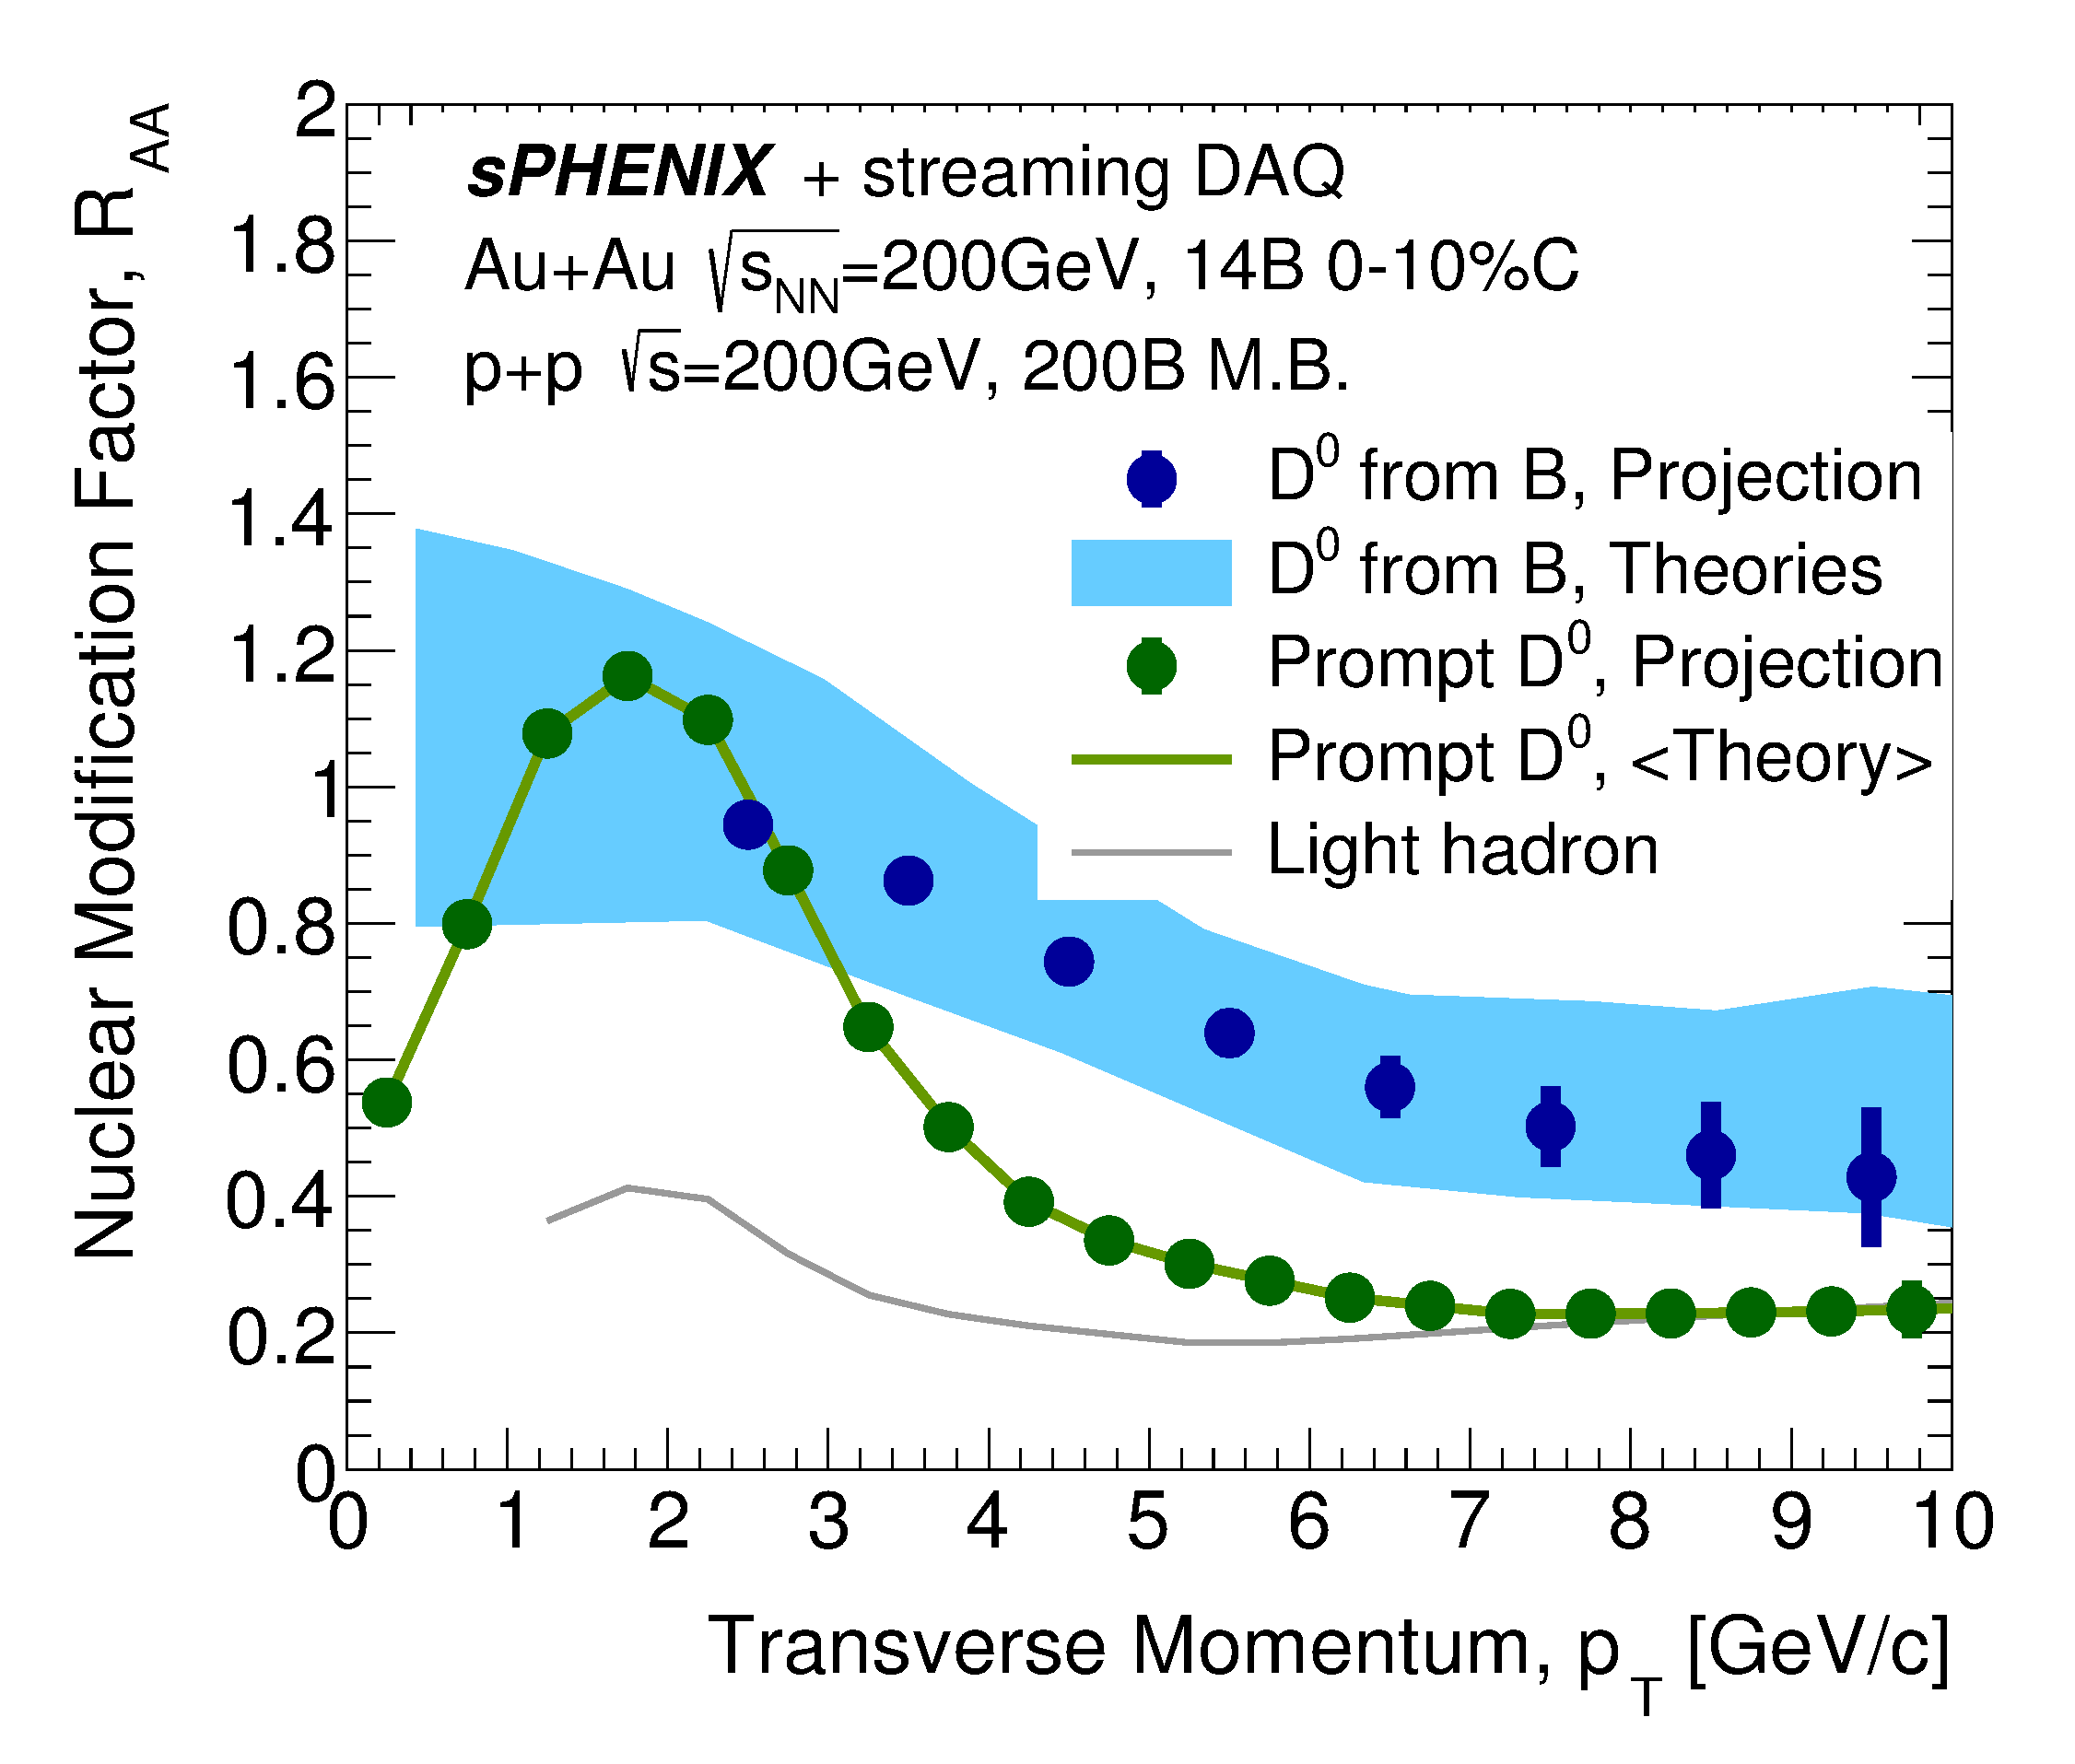
\includegraphics[width=.49\linewidth]{figs/RAA_DB_theory_root_RAADB_pp200B.pdf}
% % 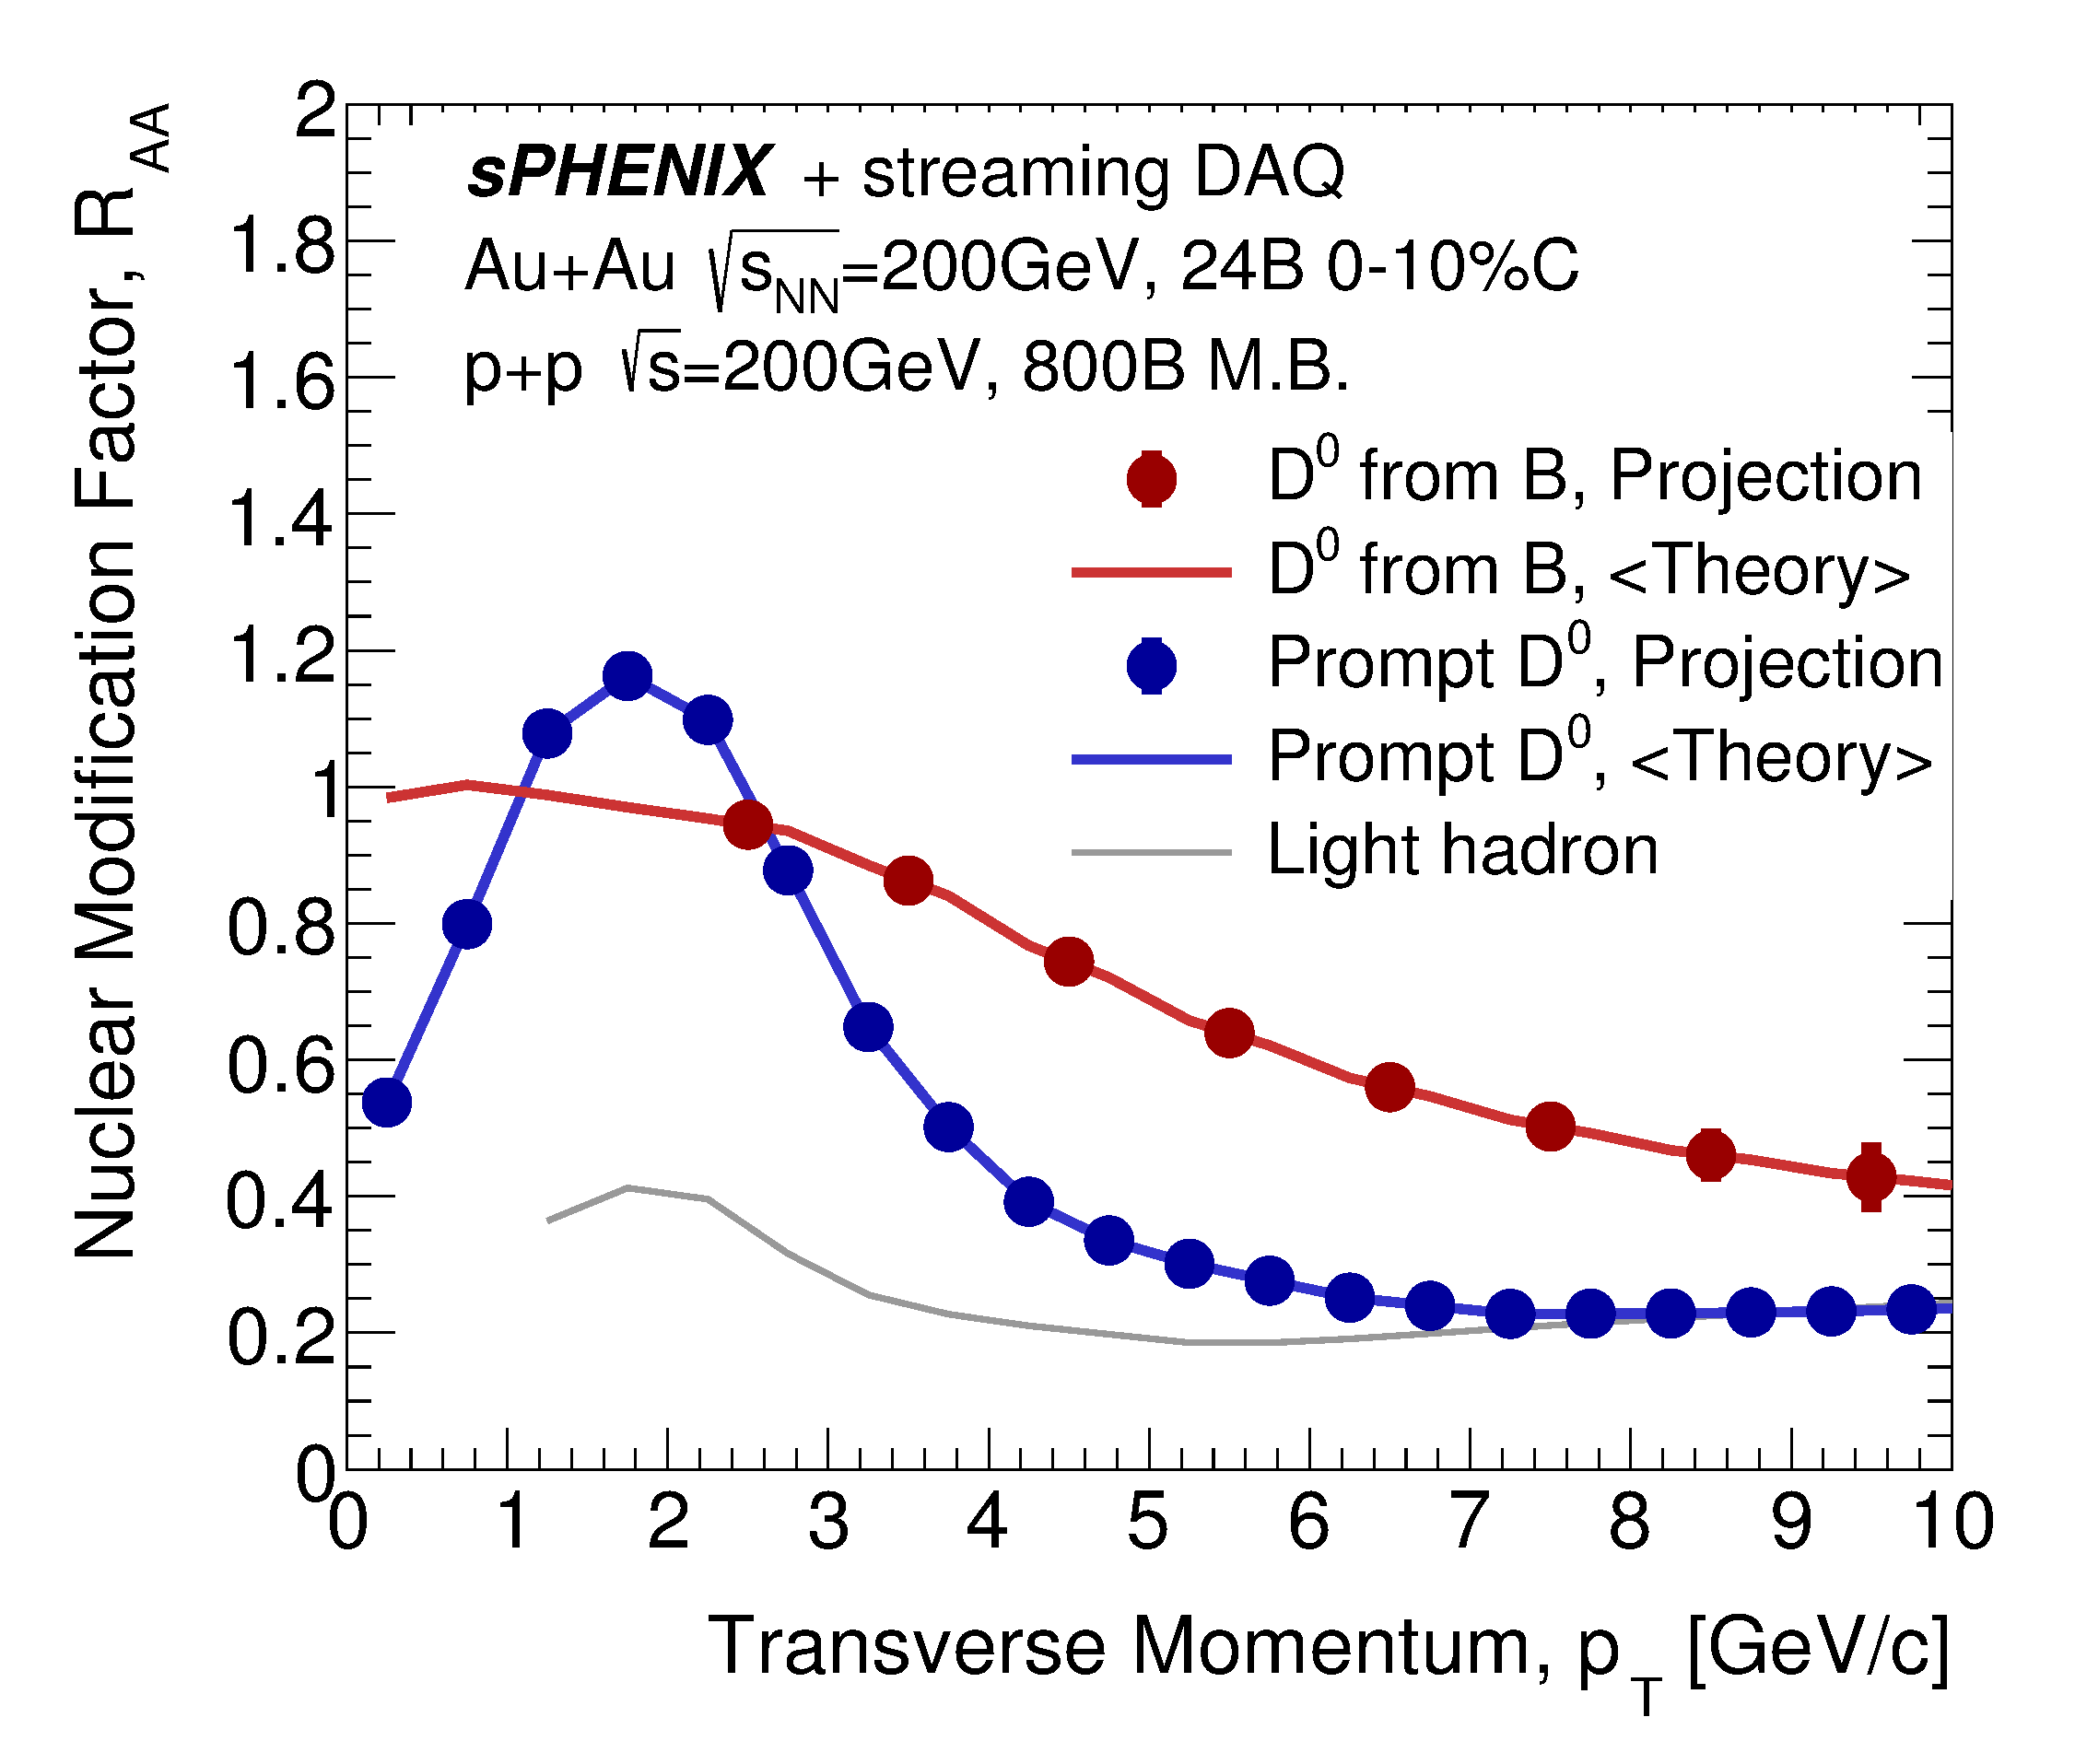
\includegraphics[width=.49\linewidth]{figs/RAA_DB_theory_root_RAADB.pdf}
% \caption{Statistical projections of $R_AA$ for $D^0$ from $B$ decays for Year-2 data taking.}
% \label{fig:RAA-D0}
% \end{center}
% \end{figure}


(Moved from streaming readout section, need rewritten....)
The currently envisioned sPHENIX experiment is designed to take large statistics of calorimeter triggered events in the \pp collisions, which will sample 2 trillion delivered \pp collisions in the vertex acceptance of the silicon tracker (18\% of all collisions) []. For observables that utilize calorimeter for analysis, a trigger can usually be designed, such as leptonic decays at higher $p_T$, jets, photon, and their correlation observables. However, low-$p_T$  ($<10$~GeV$/c$) HF hadrons usually decay hadronically and leave relatively low signals in the calorimeters when compared with the underlying event. Therefore, they cannot be efficiently collected via calorimeter triggers, which have a hadron energy threshold of 10 GeV. Therefore, in the currently envisioned sPHENIX detector, there is no efficient way in triggering such events in the \pp collisions. And in the 15 kHz sPHENIX trigger bandwidth, one would only reasonable request around few kHz of the minimum bias \pp trigger for this new program. Assuming 50\% vertex range selection purity , 1 kHz M.B. trigger leads to recording $2\times10^{-4}$ of the delivered luminosity . This translates to quite limited statistics for these rare low-$p_T$ HF signals as quantified in Table X [Need table].
This upgrade carries out the upgrade enabling the collection of a sufficient amount of minimum bias \pp events. That is 10\% delivered luminosity (see next Chapter), 200 billion events in vertex tracker acceptance, which is a factor of 500 improvements. This dataset enables a comprehensive low-$p_T$ hadron program as discussed in this subsection. The analysis for these HF hadronic channels does not require calorimeter information. Instead, they can be identified with the precision tracking detectors of sPHENIX (at $p_T$=5 GeV$/c$, $\sigma(p)/p=1\%$, $\sigma(DCA)<10$~$\mu$m ) via a combination of decay topology and invariant mass, as demonstrated for even the busiest events of Au+Au collisions through detailed simulation studies in [?]. 
 
The non-prompt $D^0$ meson production is a clean channel to access b-quark via its decay chain. Using tracker data alone, both prompt and non-prompt $D^0$ can be reconstructed via the invariant mass and a multi-variable classification algorithm based on the decay topology, including the distance of closest approach ($DCA$) of tracks, the closeness between tracks, decay length and angle, as demonstrated in a worse background situation (A+A) in []. Together with the sPHENIX Au+Au dataset, this upgrade will enable the first precision measurement of nuclear modification of the B observable at RHIC via the non-prompt $D^0$ as highlighted in Figure~\ref{fig:RAA-D0}. Similar measurement will be expanded to the exclusive decay modes such as $B^+ \rightarrow \pi^+ (D^0 \rightarrow \pi^- K^+)$) (~1k events expected).

With the extensive, inclusive dataset, the SRO upgrade will further enable novel highly differential observables, such as the $c$-quark correlation measurement by detecting pairs of $D^0$ mesons. 500k $D^0$ pairs will be recorded with the upgraded DAQ. Together with the planned Au+Au data, such dataset for Charm correlations will provide a unique handle in quantitatively understanding the diffusion of c-quarks in QGP []. 

\subsection{Heavy Quark Hadronization}


% \begin{figure}[htbp]
% \centering
% 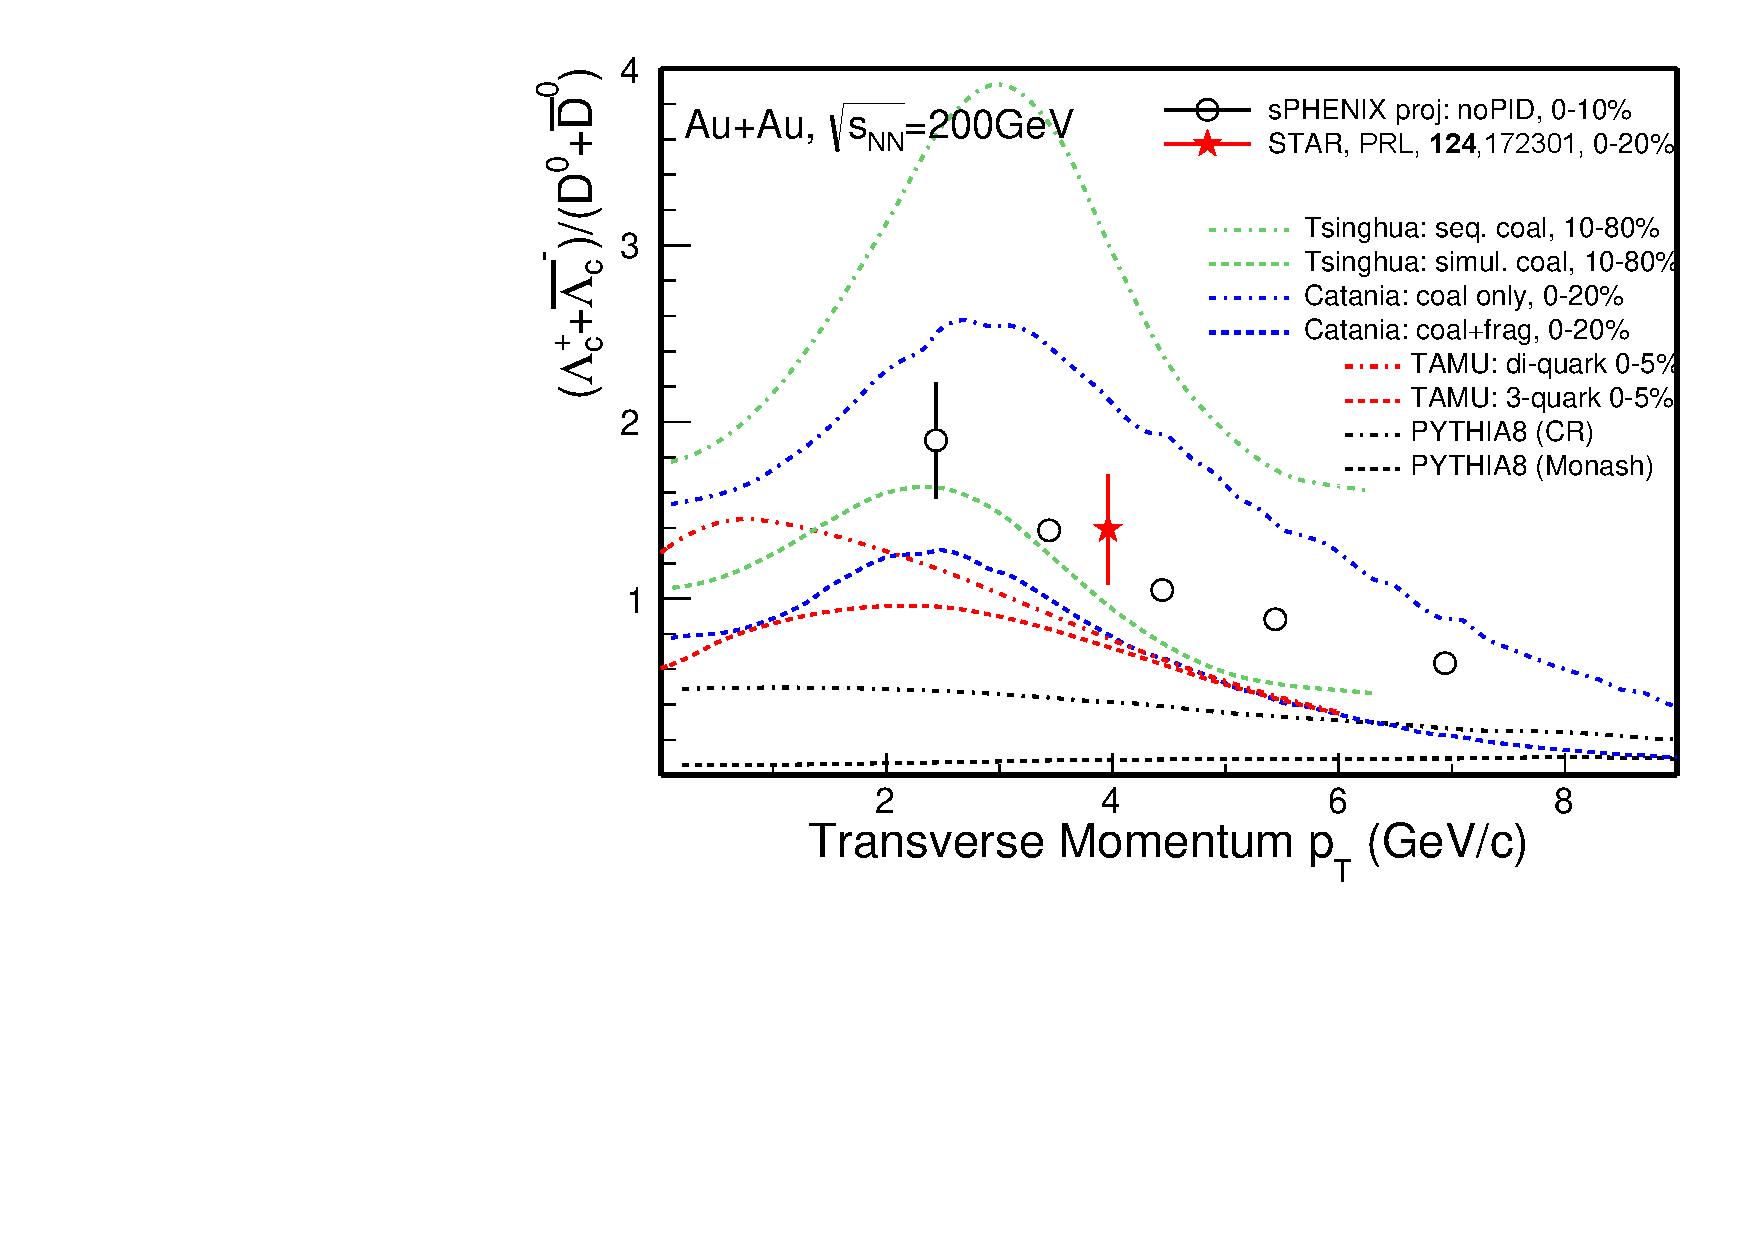
\includegraphics[width=0.48\textwidth]{figs/LcD0_proj_0_10_24B_Update.pdf}
% \caption{Projected statistical uncertainties of $\lambda_c$ to $D^0$ ratio.}
% \label{fig:HF-Lc}
% \end{figure}

\begin{figure}[htbp]
\begin{center}
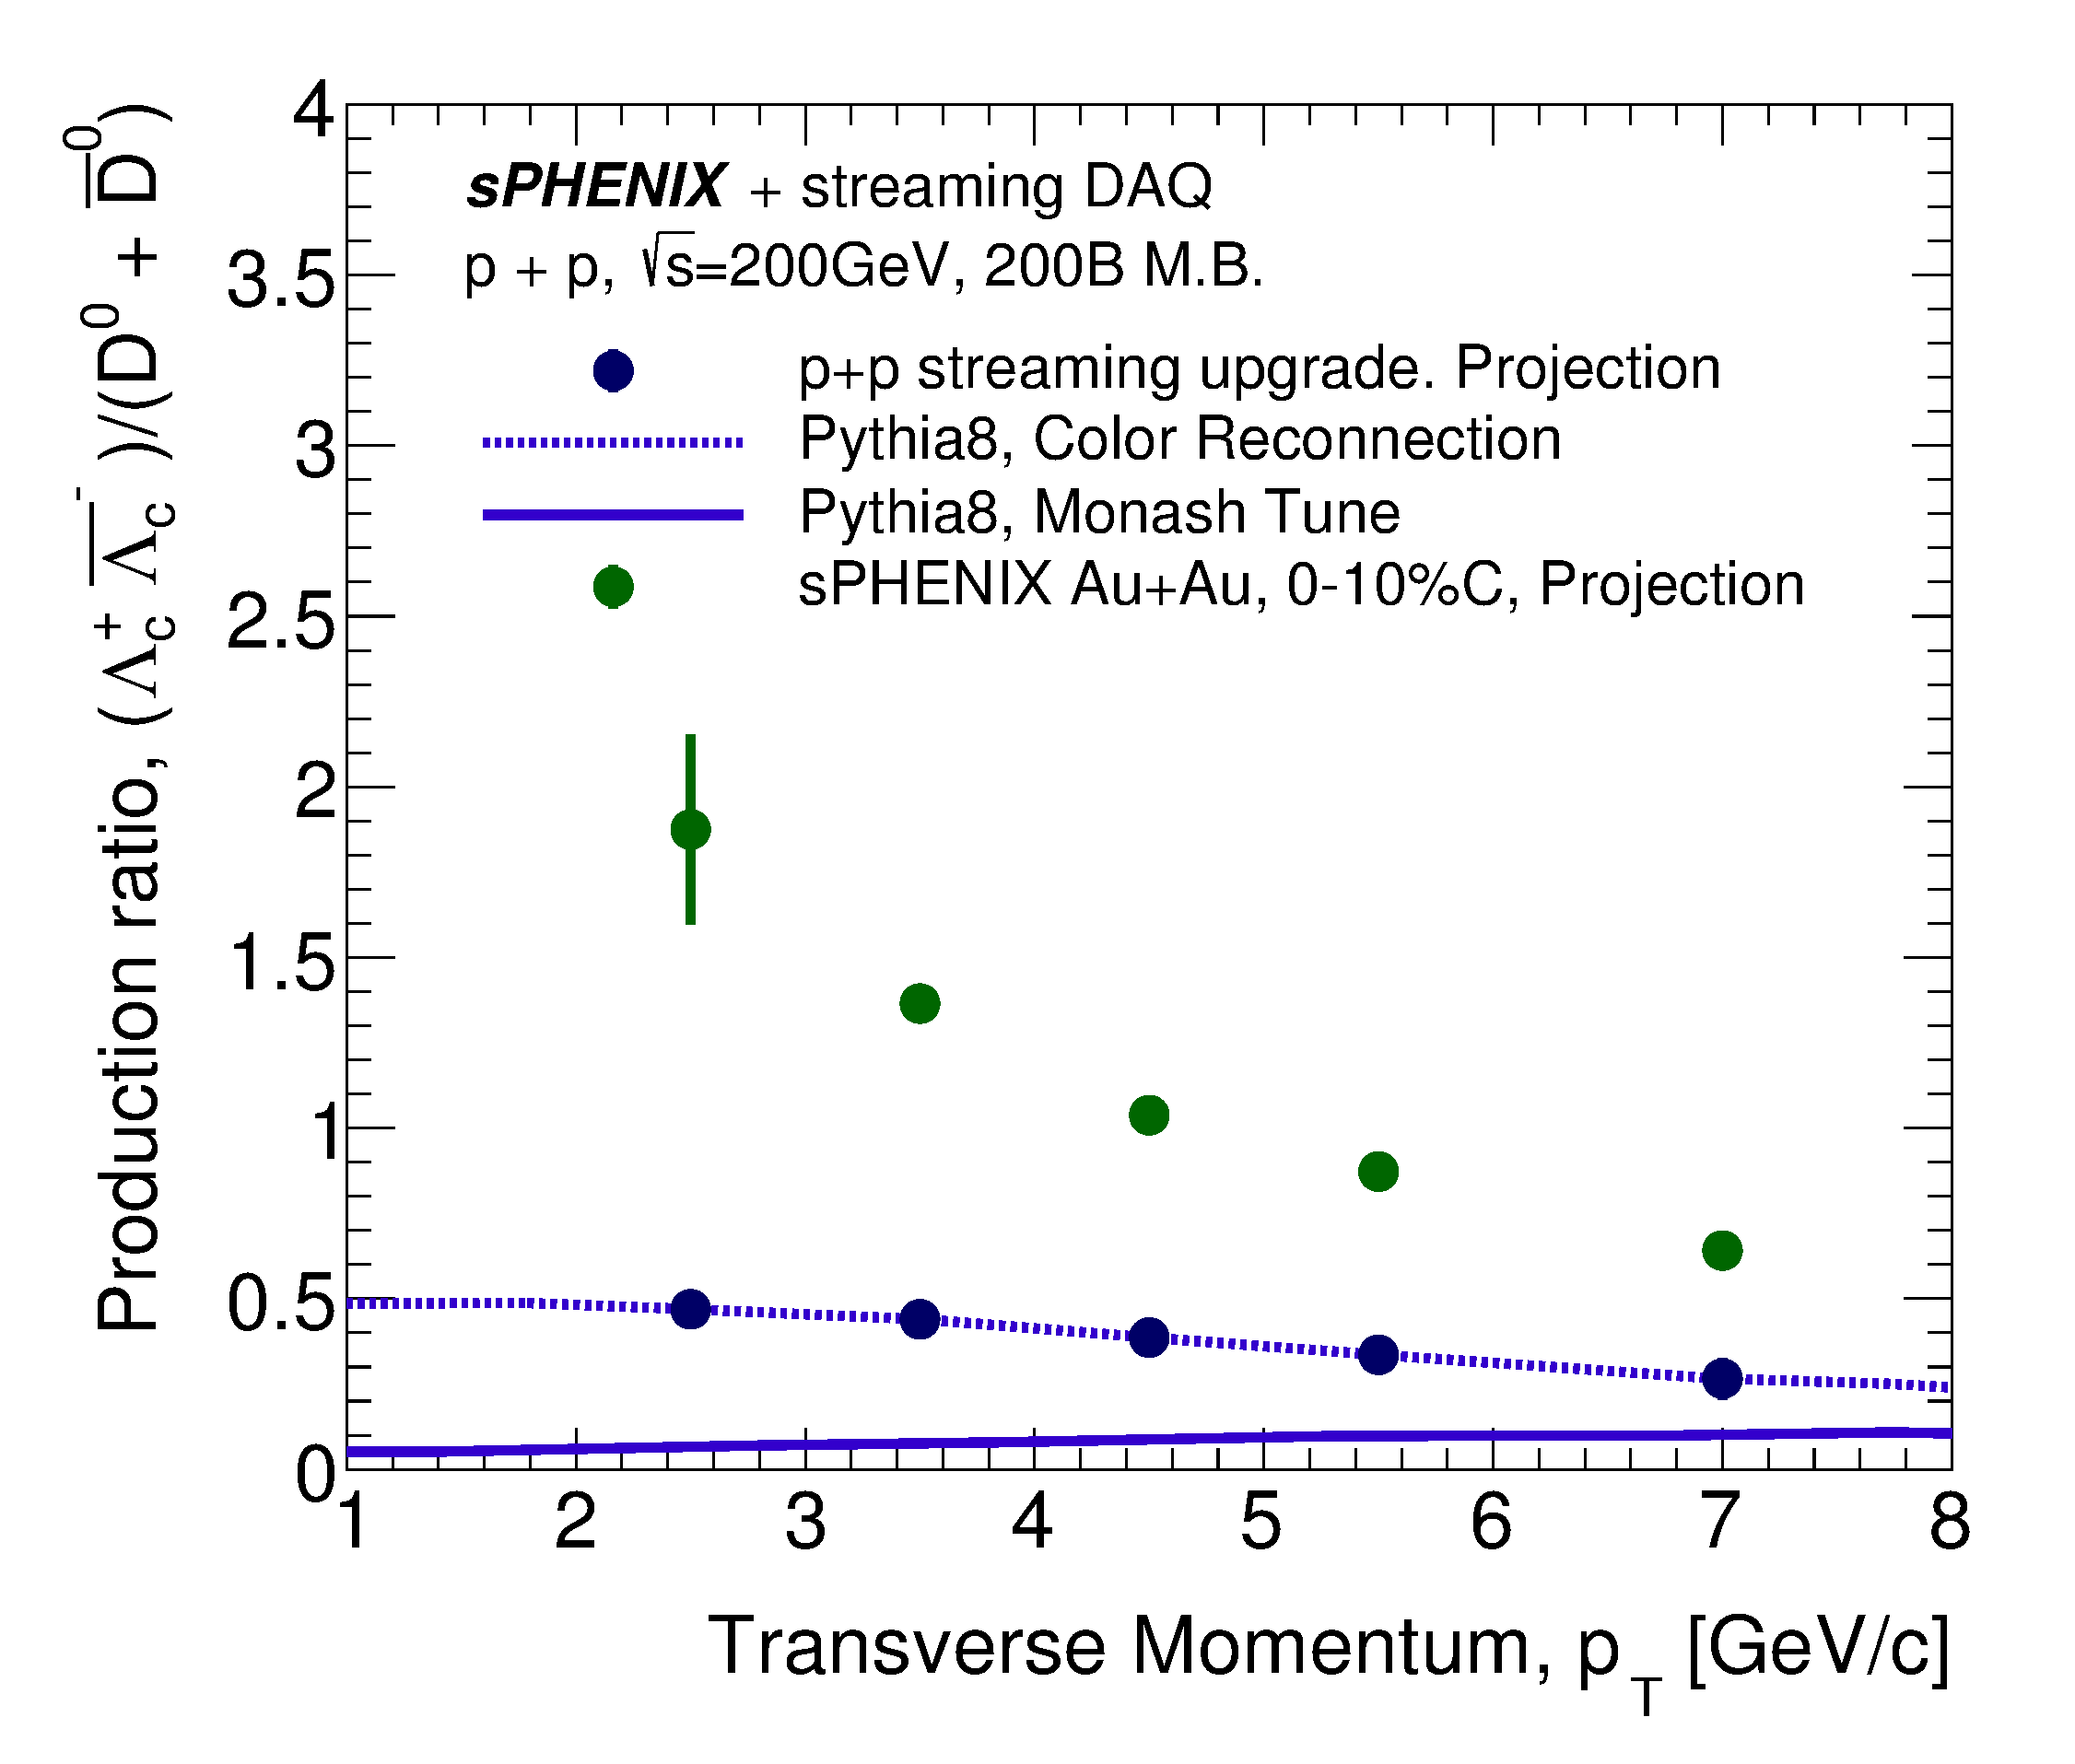
\includegraphics[width=.49\linewidth]{figs/RAA_DB_theory_root_LcD0Ratio_pp200B.pdf}
% 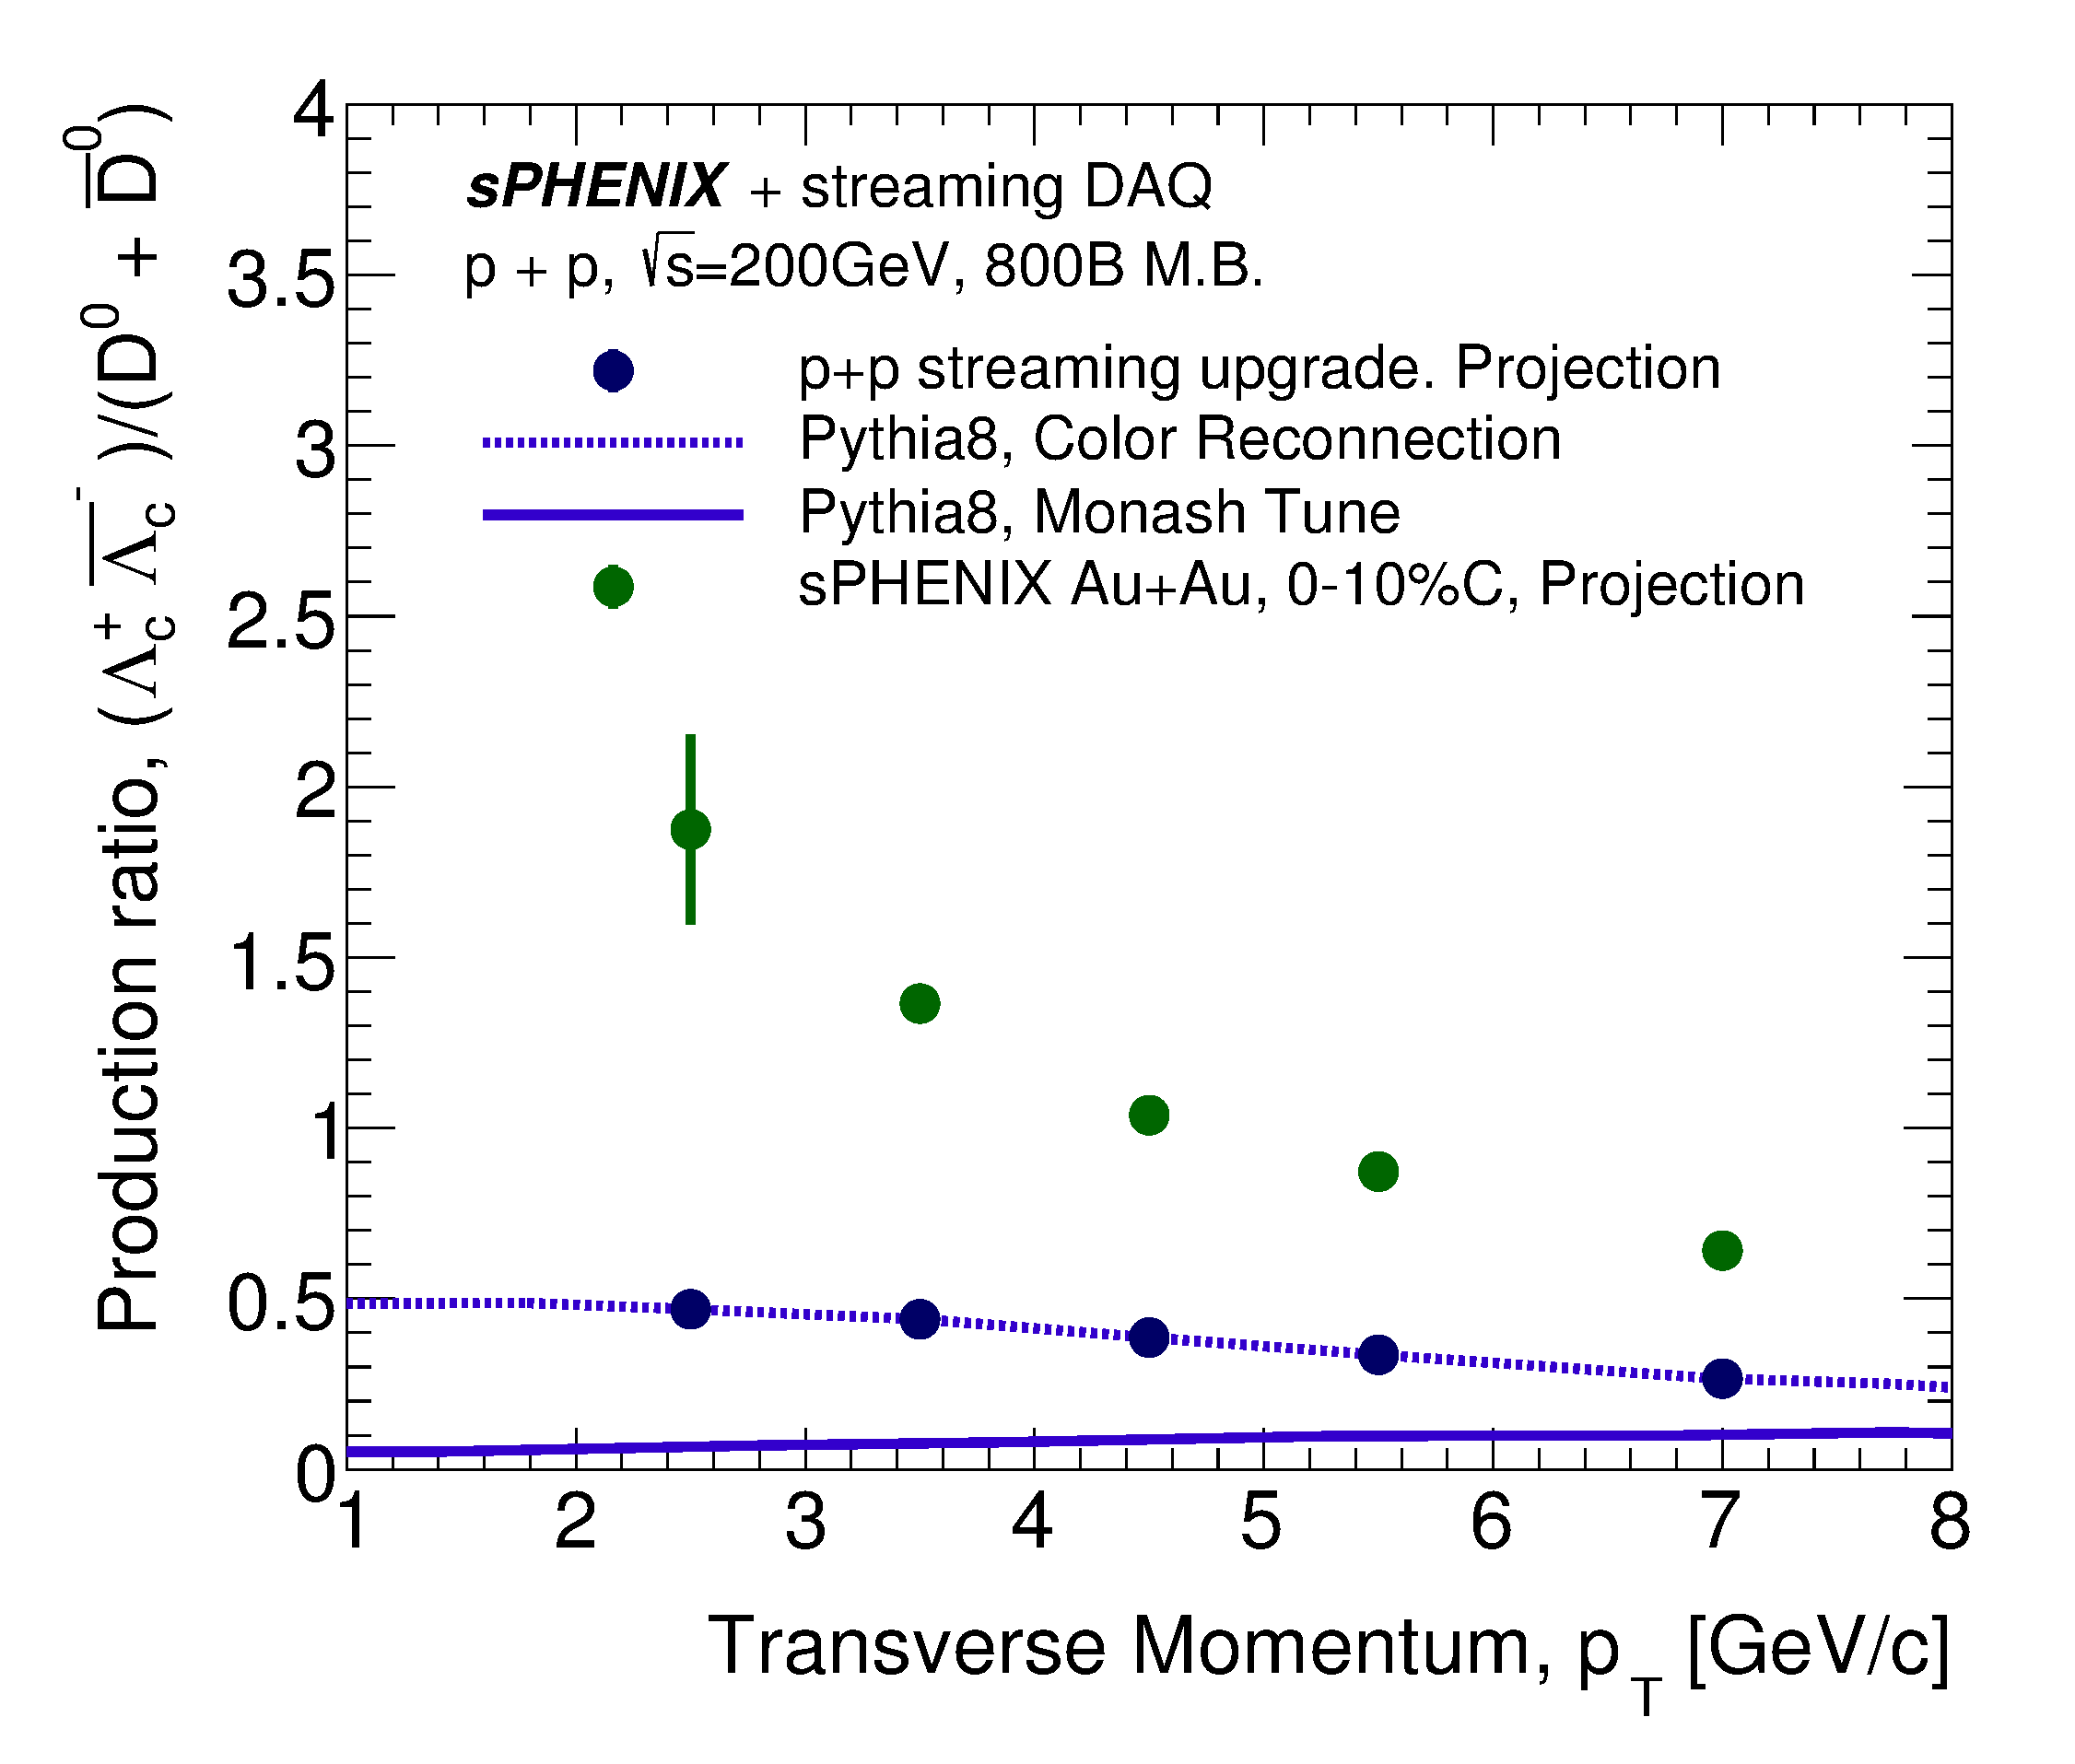
\includegraphics[width=.49\linewidth]{figs/RAA_DB_theory_root_LcD0Ratio.pdf}
\caption{(need STAR published point) Statistical projections of $\Lambda_c/D$ ratio for Year-2 data taking.}
\label{fig:Lc-D0}
\end{center}
\end{figure}



Recent RHIC and LHC data indicate significant enhancements of the  $\lambda_c$ baryon to $D^0$ meson production ratio in \pp,  \pA and \aa  collisions []. However, the reference $\Lambda_c/D$ ratio in the \pp collision is missing at the RHIC energies, and the current model predictions differ significantly. As shown in Figure~\ref{fig:Lc-D0}, this upgrade will enable the first measurement of the $\Lambda_c/D$ in \pp collisions at RHIC and provide the critically missing link to quantitatively understand the enhancement of the charmed baryon/meson production ratio and therefore charm hadronization in the QGP []. 


 





\section{Cold QCD Physics}
\label{sec:ColdQCD}

The sPHENIX detector, designed to study QGP with jet, photon and heavy flavor probes, with its trigger capabilities and high DAQ rate capabilities, will provide key opportunities for cold QCD measurements. These include a broad range of physics measurements with transversely polarized beams, and studies of transverse momentum effects and hadronization in $p+p$ and $p+A$ collisions. 

%The main emphasis of the RHIC Spin program has been measurements of the gluon polarization in longitudinally polarized proton collisions. RHIC experiments discovered a significant gluon polarization in the gluon momentum fraction range $x>0.05$. Even with the future EIC data expected to precisely measure $\Delta G$ in the lower x region, RHIC data will remain a significant contributor at $x>0.05$. However, any significant improvement of $\Delta G$ measurements, compared to existing RHIC data (published and being analyzed), requires significant integrated luminosity (at least a few hundred pb$^{-1}$), which is not anticipated in the sPHENIX 3-year running scenario. Therefore in this document we focus on the measurements with transversely polarized beams.

\subsection {Transverse Spin Measurements}

In recent years, transverse spin phenomena have gained substantial attention. The nature of significant transverse single spin asymmetries (TSSAs) in hadron collisions, discovered more than 40 years ago at low center of mass energy ($\sqrt{s}$=4.9 GeV), and then confirmed at higher energies up to $\sqrt{s}$=500 GeV and $p_T \sim 7$~GeV/$c$ at RHIC, has not yet been fully understood. Different mechanisms are suggested to explain such asymmetries, involving initial-state and final-state effects, in the collinear or transverse-momentum-dependent (TMD) framework. These descriptions have deep connections to nucleon partonic structure and parton dynamics within the nucleon, as well as spin-momentum correlations in the process of hadronization.

The TSSAs in direct photon and heavy flavor production probe the gluon dynamics within a transversely polarized nucleon, described by the trigluon correlation function in the collinear twist-3 framework, which is connected with the gluon Sivers TMD parton distribution function (PDF), thus far poorly constrained. The Sivers function correlates the nucleon transverse spin with the parton transverse momentum.

The projected uncertainties for the midrapidity direct photon TSSA compared to theoretical calculations are shown in Figure~\ref{fig:AN_dp} . The direct photon sample here will be collected with an EMCal-based high-energy cluster trigger. 
%Asymmetry measurements in $D^0$ meson production through its hadronic decay will be done from a minimum bias (MB) sample collected with streaming readout. Figure~\ref{fig:AN-D0} shows the projected uncertainties for such a measurement.
The new capability of the sPHENIX streaming DAQ (detailed in Section~\ref{sec:streaming_readout}) enables a high precision measurement of $D^0$ TSSA in the mid-rapidity region as shown in Figure~\ref{fig:AN-D0}. 
%This observable is a unique probe of the twist-3 tri-gluon correlation function and gluon Sievers effect in the polarized proton, which opens a new window into the dynamics of gluons in hadrons [Reference to be updated]. 

\begin{figure}[htbp]
\centering
\includegraphics[width=0.60\textwidth]{figs/AN_dp_sphenix.pdf}
\caption{Projected statistical uncertainties for dir. photon $A_N$}
\label{fig:AN_dp}
\end{figure}

\begin{figure}[htbp]
\begin{center}
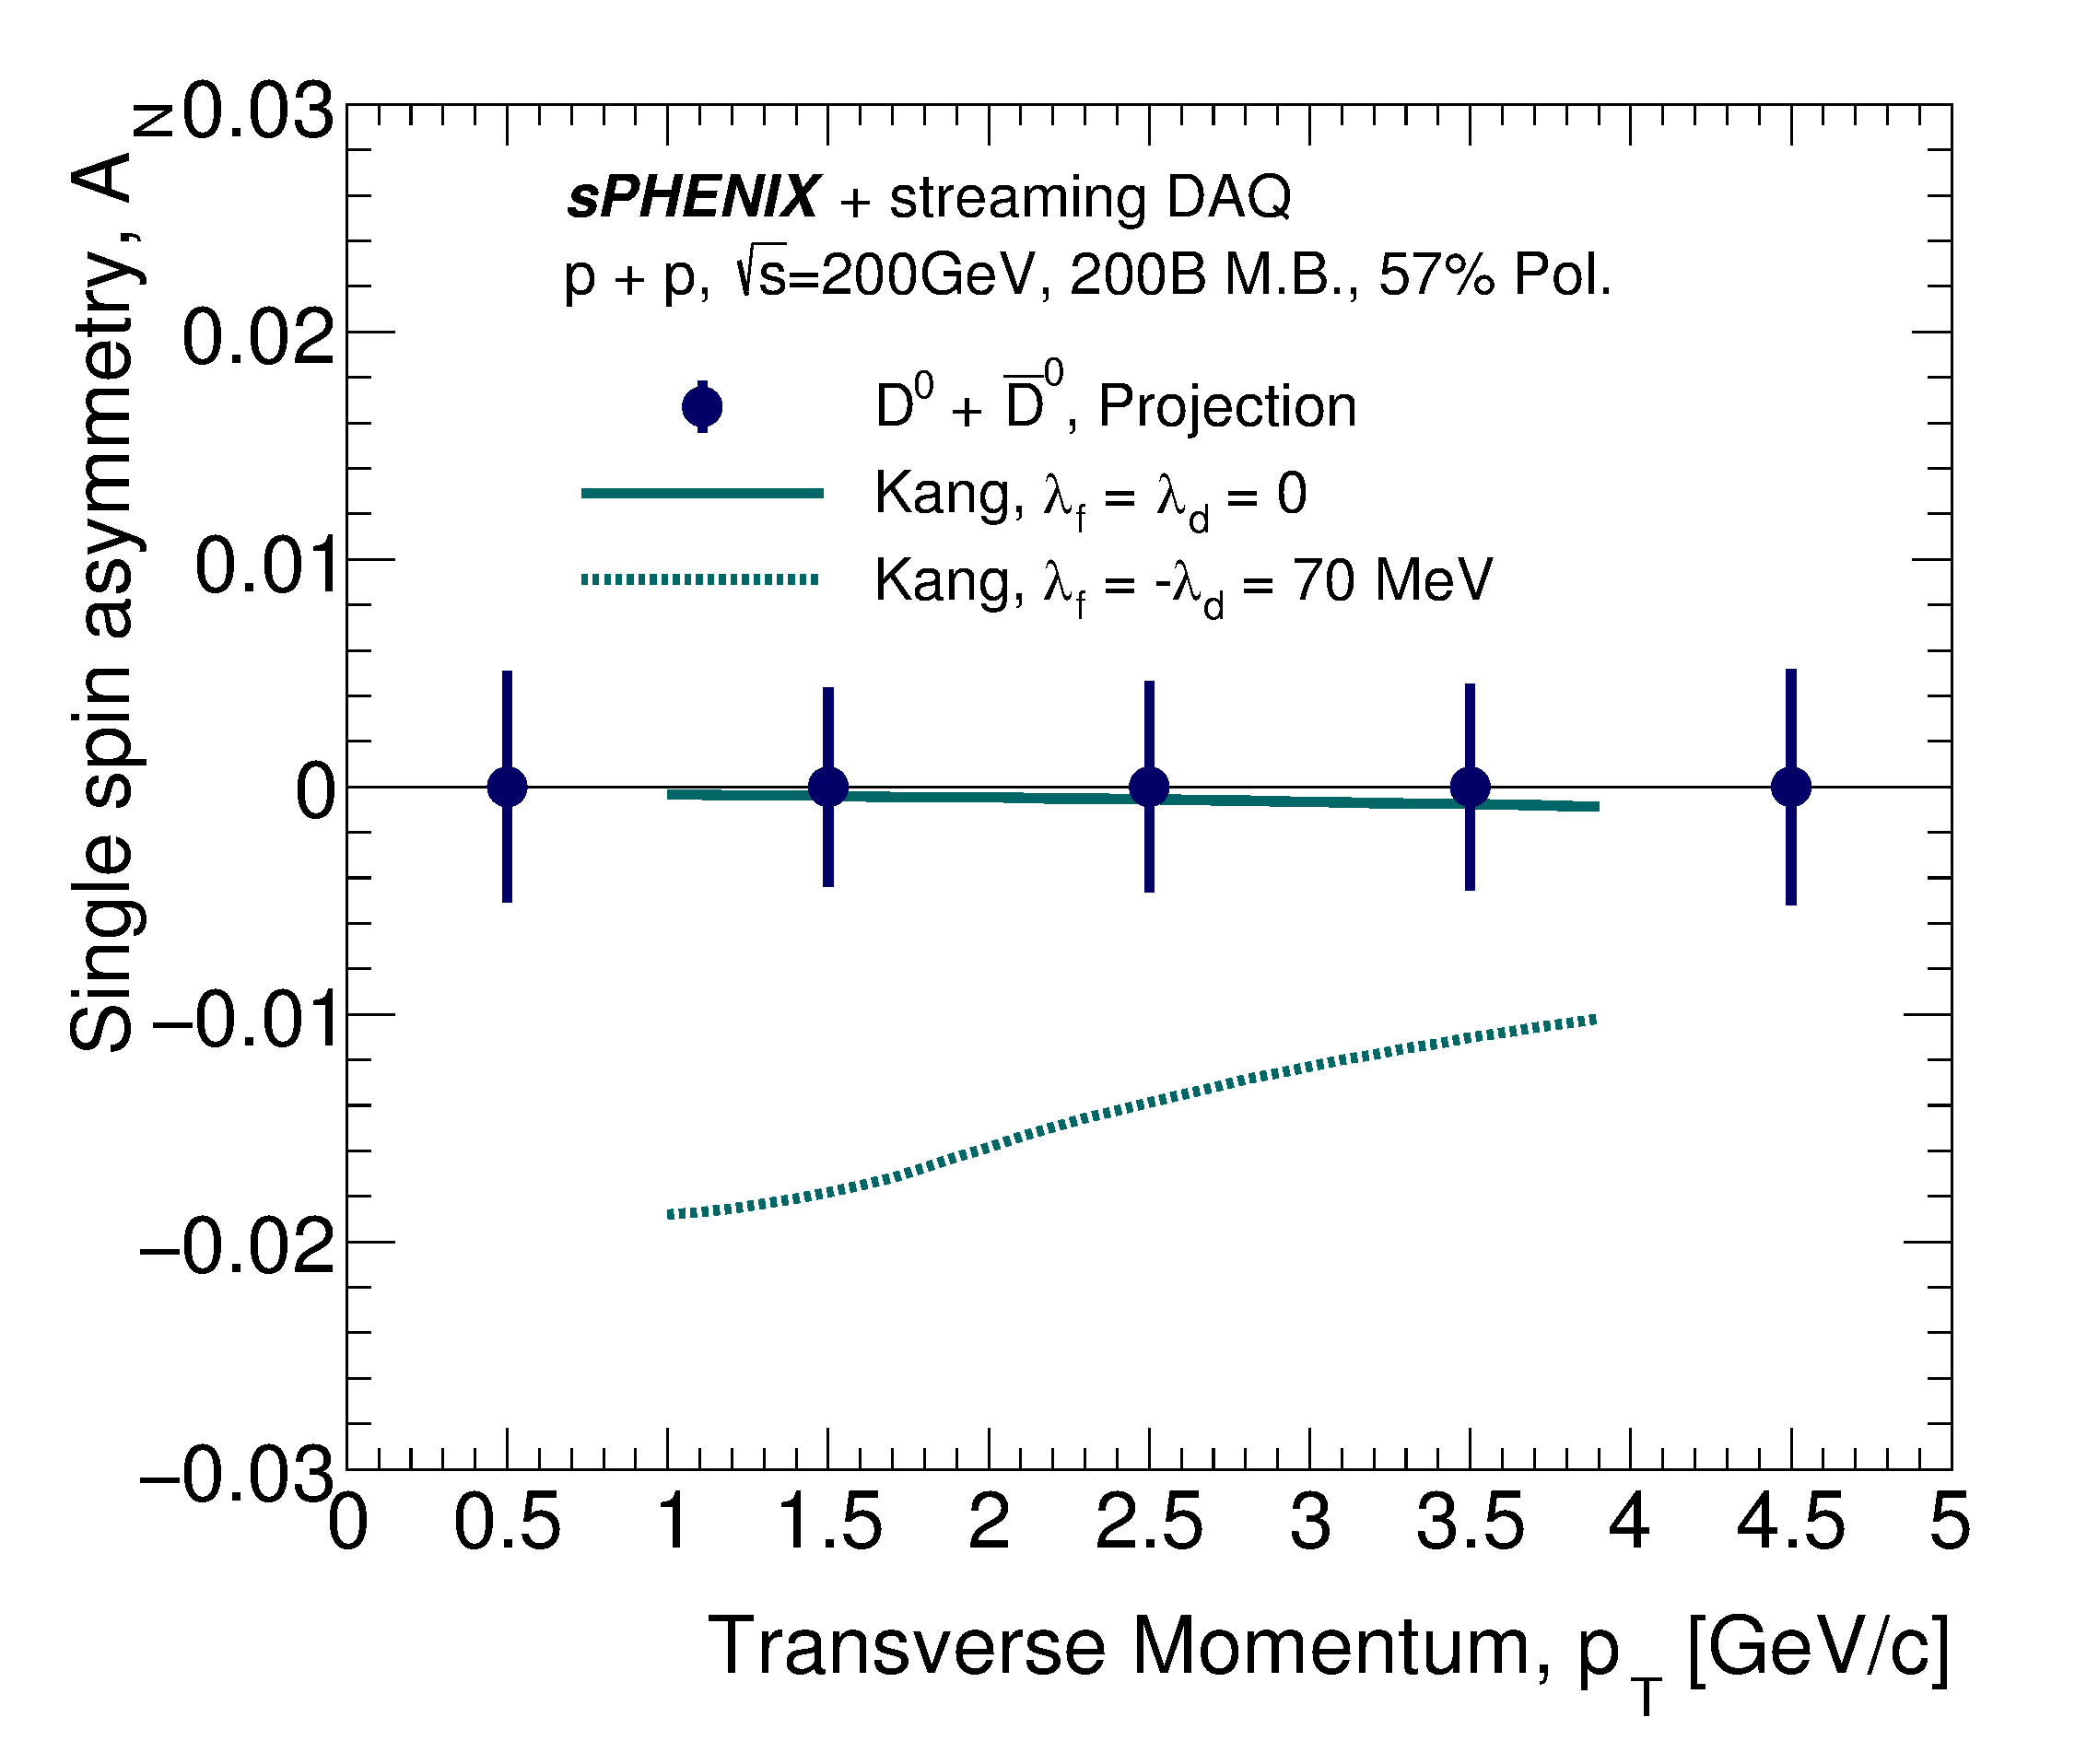
\includegraphics[width=.49\linewidth]{figs/RAA_DB_theory_root_AN_D0D0bar_pp200B.pdf}
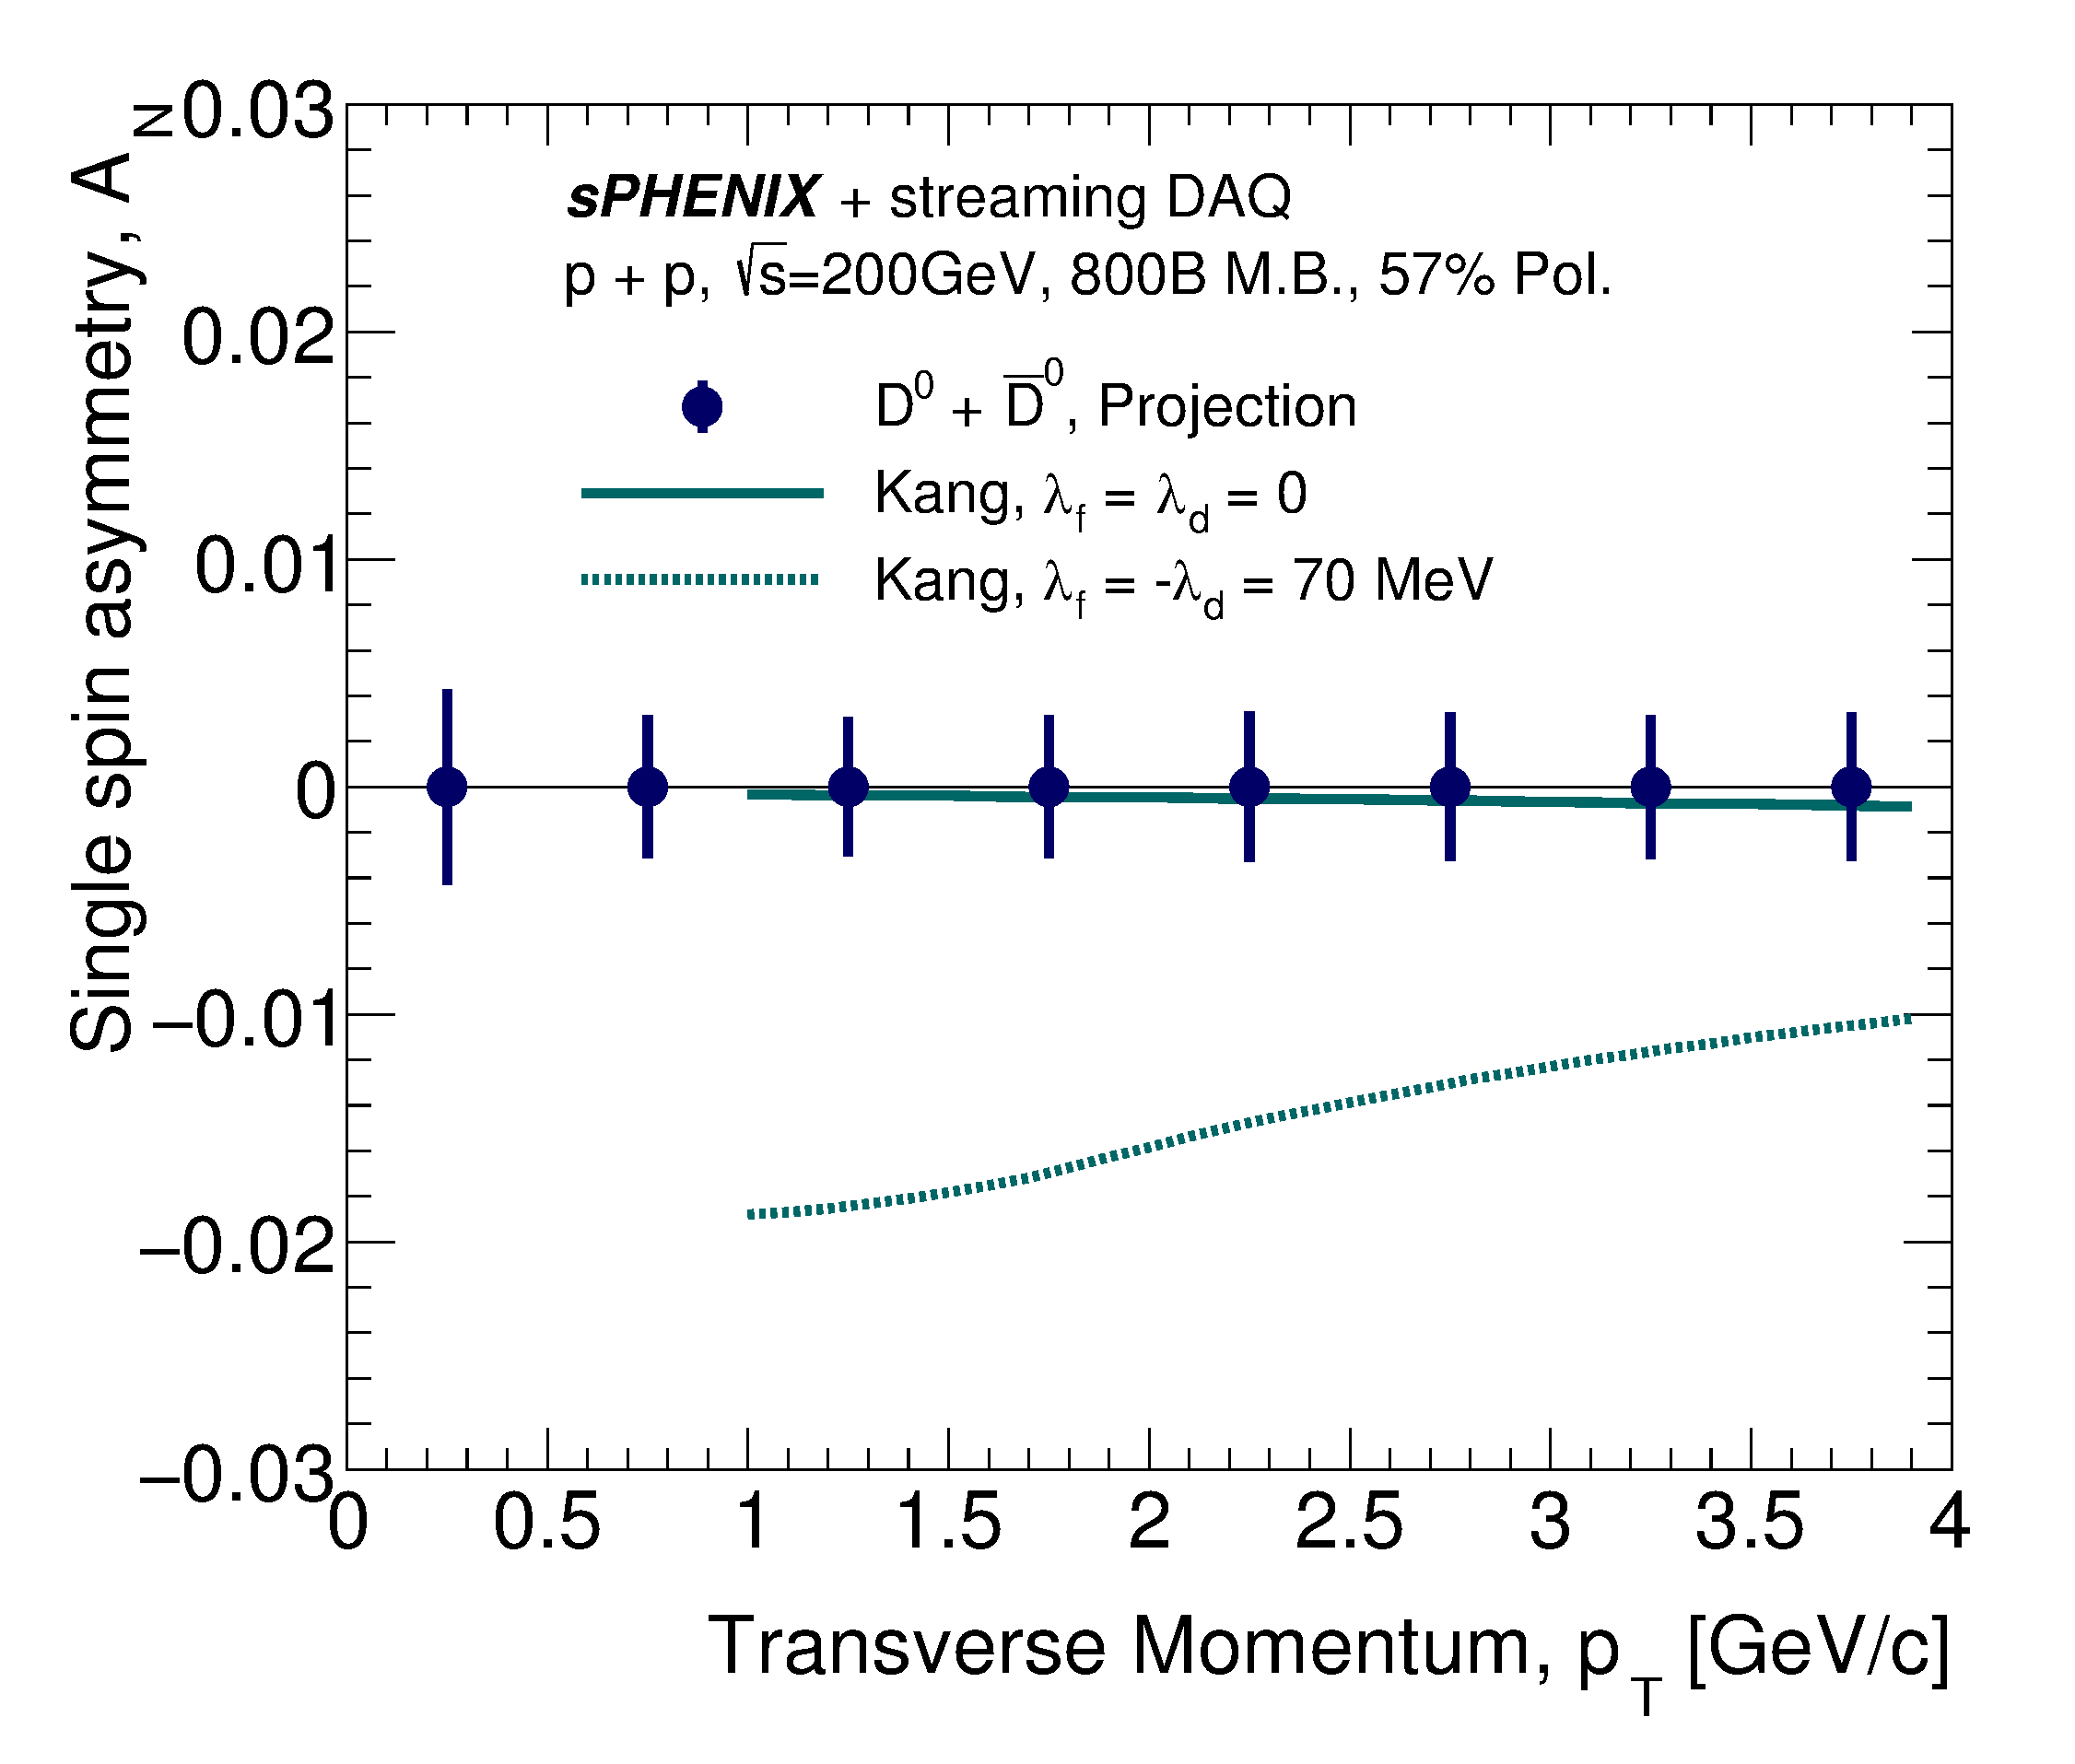
\includegraphics[width=.49\linewidth]{figs/RAA_DB_theory_root_AN_D0D0bar.pdf}
\caption{[To be updated with lumi numbers] Statistical projections of transverse spin asmmetry for the $D^0$ mesons for Year-2 and Year 2+4 data taking.}
\label{fig:AN-D0}
\end{center}
\end{figure}

Another interesting channel related to the Sivers effect is the inclusive jet TSSA, which has not yet been measured at central rapidity. sPHENIX can provide high precision measurements with uncertainties on the level of a few times $10^{-4}$. While the opposite sign contribution of up and down quarks to Sivers asymmetry is expected to suppress the measured TSSA, tagging the leading hadron charge will preferentially enhance the contribution from fragmenting up or down quarks, and therefore will enable the flavor-separated measurements in the central rapidity kinematics.

Dijet measurements allow for direct access to parton intrinsic transverse momentum $k_T$. Again, charged tagging will enhance the effect from either up or down quarks, which otherwise will be essentially cancelled out. Recent STAR preliminary results showed a nonzero effect for charge-tagged jets. sPHENIX as a dedicated detector for jet and photon measurements is expected to significantly contribute to these measurements and to extend it to photon-jet measurements, which essentially isolate the quark-gluon scattering process at leading order, thus giving access to the gluon Sivers effect.

Another possible origin of the observed TSSAs is the Collins mechanism, which correlates the transverse polarization of a fragmented quark to the angular distribution of hadrons within a jet. This gives access to the transversity distribution in the proton, which can be interpreted as the net transverse polarization of quarks within a transversely polarized proton. Along with the unpolarized PDF and helicity PDF, transversity is one of three leading-twist PDFs, least known at the moment. The integral in $x$ over the valence quark transversity distribution defines the tensor charge, a fundamental value calculable in lattice QCD, therefore enabling the crucial comparison of experimental measurements with ab-initio theoretical calculations.

Measuring angular distributions of dihadrons in the collisions of transversely polarized protons, couples transversity to the so-called “interference fragmentation function” (IFF) in the framework of collinear factorization. The IFF describes a correlation between the spin of an outgoing quark and the angular distribution of a hadron pair that fragments from that quark.  A comparison of the transversity signals extracted from the Collins effect and IFF measurements will explore questions about universality and factorization breaking.

The first nonzero Collins and IFF asymmetries in $p+p$ collisions have been observed by STAR collaboration at midrapidity, and shown to be invaluable to constrain the transversity distribution. sPHENIX, with its excellent hadron and jet calorimetric trigger capabilities coupled with its high-rate DAQ capabilities, is expected to deliver high-statistics samples for both Collins and IFF asymmetries. sPHENIX's capability to collect a significant
data sample with streaming readout will allow us to extend the charged dihadron measurements for IFF asymmetries from the barrel region ($|\eta|<1$) to more forward kinematics up to $\eta=2$. 
%Fig.* shows projected uncertainties for IFF asymmetries [hopefully we'll get them].


\subsection {Transverse Spin: pp vs pA}

$p\uparrow$+A collisions at RHIC provide unique opportunities to study spin effects in a nuclear environment. These studies may provide new insights into the origin of the observed TSSAs and a unique tool to investigate the rich phenomena behind TSSAs in hadronic collisions. TSSAs measured in polarized $p$+A collisions moreover offer a new approach to studying small-system collisions, in which numerous surprising effects have been observed in recent years.

First RHIC results from the 2015 RHIC run showed a puzzling evolution of the TSSA from $p+p$ to $p+Al$ and then $p+Au$. While STAR's preliminary result for $\pi^{0}$ asymmetry in forward rapidity (with $0.2<x_F<0.7$) showed no significant nuclear dependence, PHENIX's positively charged hadron asymmetries in the intermediate rapidity range (with $0.1<x_F<0.2$) discovered a strong nuclear dependence in the TSSA, from $A_N \sim 0.03$ in $p+p$ collisions to a value consistent with zero in $p+Au$ collisions. No clear explanation for such a behavior has been offered at the moment. Obviously, more data, differentiated in $p_T$ and $x_F$, would be highly desirable. sPHENIX is able to collect much more data in this channel, with fine binning, which is expected to provide crucial information on the nature of TSSAs in hadronic collisions and on understanding of the spin probe - nucleus interaction, a novel topic directly associated with RHIC's unique ability to collide polarized protons with nuclei.

Figure~\ref{fig:AN_h} shows the projected uncertainties for sPHENIX, based on MB data collected with the streaming readout. The sPHENIX tracking system will provide us with charged hadron measurements in the pseudorapidity range up to $\eta=2$, which overlaps with the PHENIX range, where the strong nuclear effect was observed ($1.2<\eta<2.4$).

\begin{figure}[htbp]
\centering
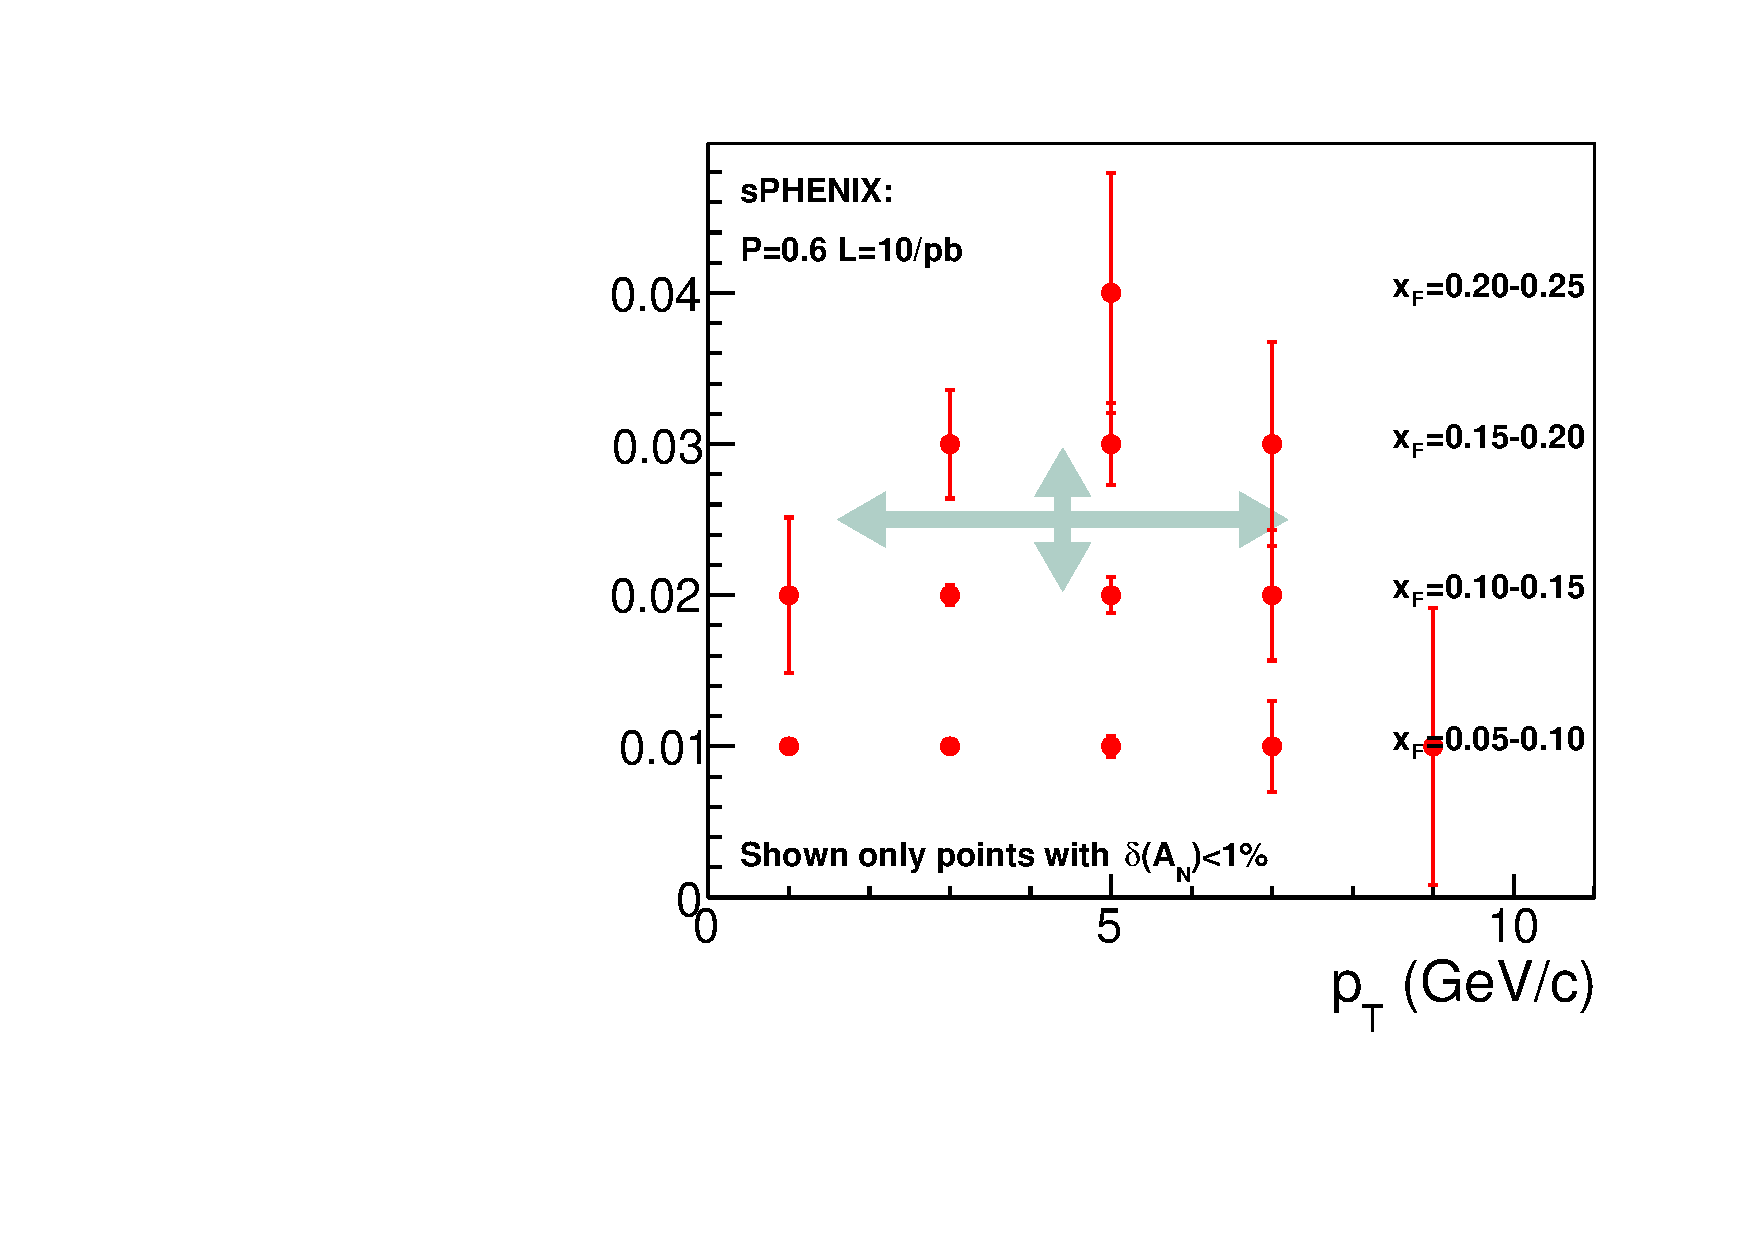
\includegraphics[width=0.60\textwidth]{figs/sphenix_han.pdf}
\caption{Projected statistical uncertainties for $h^{+}$ $A_N$ in $p+p$ collisions, for data collected with streaming readout; similar uncertainties are expected from $p+Au$ data; green arrows indicate the stat. uncertainty and the $p_T$ coverage of the PHENIX data point (with $0.1<x_F<0.2$).}
\label{fig:AN_h}
\end{figure}

The other measurements (e.g. Collins and IFF asymmetries) will also be compared between $p+p$ and $p+A$ systems and may potentially bring new surprises.


\subsection {Unpolarized Measurements}

A number of cold QCD measurements that do not require beam polarization are planned in $p+p$ and $p$+A collisions. Hadronization studies will be performed with hadron-in-jet measurements, multidifferential in momentum fraction $z$ of the jet carried by the produced hadron, in the transverse momentum $j_T$ of the hadron with respect to the jet axis, and in the angular radial profile $r$ of the hadron with respect to the jet axis. This includes studies for both light quark and heavy quark hadrons. Comparison of $p+p$ and $p$+A collisions will provide information on the nuclear modification of hadronization processes. Measurements performed by PHENIX of nonperturbative transverse momentum effects and their nuclear modifications in back-to-back dihadron and photon-hadron correlations, will be extended to dijet and photon-jet measurements in sPHENIX.  These measurements will help to separate the effects associated with intrinsic parton momentum $k_T$ in the nucleon or nucleus and fragmentation transverse momentum $j_T$. These correlation measurements may also help to probe theoretically predicted factorization breaking effects within the transverse-momentum-dependent framework. Upsilon and J/$\Psi$ polarization measurements will shed further light on heavy quarkonium production mechanisms.

%\chapter{Species Scan}
\label{chap:species_scan} - jln, this needs to all go into the out years... below.
\chapter{Beam Use Proposal 2026-2027}
\label{chap:beam_use_proposal_extra}

In this Chapter we provide details on a potential additional two years of running in 2026-2027 that presents a further return on investment in sPHENIX and also the entire RHIC program.   We highlight if such a window of opportunity arises this would represent the last opportunity for data taking in heavy-ion mode in this energy regime in our lifetime. 

\section{Proposal Summary}

The sPHENIX proposal for such a potential window of opportunity is summarized in Table~\ref{tab:summary2627}.   The two years assume 28 cryo-weeks in each and with a sPHENIX uptime of 80\% with detector operations having reached a mature state.   Projected luminosities are documented by these years 2026 and 2027 by C-AD.  For completeness we detail in the cryo-weeks for the potential 2026 and 2027 runs at the end of this Chapter in Section~\ref{sec:cryo20262027}.

\begin{table}[h]
\centering
\caption{The recorded luminosity (Rec. Lum.) and sampled luminosity (Samp. Lum.) values are for collisions with z-vertex $|z|<$ 10 cm.  \label{tab:summary2627}}
\bigskip
\centering
\begin{tabular}{ | c | c | c | c | c | c | c  | }
\hline
Year & Species & $\sqrt{s_{NN}}$ & Cyro  & Physics & Rec. Lum. & Samp. Lum. \\
     &         & [GeV]           & Weeks & Weeks   & $|z|<$10~cm & $|z|<$10~cm  \\ \hline \hline
     {\bf 2026} & $p^{\uparrow}p^{\uparrow}$   & 200 & 28 & 15.5      & 1.0 \pb [10 kHz]   & 130 \pb \\ 
      & & & & & 130~\pb [100\%-$str$] & \\ \hline
 --  & O+O    & 200 & -- & 2        & 14~\nb +  47~\nb [100\%-$str$] & 47~\nb  \\ \hline
 --  & Ar+Ar   & 200 & -- & 2      & 30~\nb + 68~\nb [100\%-$str$] & 68~\nb  \\ \hline \hline
{\bf{2027}} & \auau   & 200 & 28 & 24.5 & 30 \nb [100\%-$str$/DeMux]   & 31 \nb \\ \hline
\end{tabular}
\end{table}

We highlight that key upgrades at very modest cost are a major factor increasing the physics impact of these additional years of running.   DeMultiplexing the calorimeter readout increases the Level-1 trigger accept rate to 30 kHz, doubling the rate of calorimeter data events.    Increasing the tracking detectors streaming readout to 100\% results in an order of magnitude more data than in the 2024-2025 data taking.    These upgrade options are detailed in Chapter~\ref{chap:readout}.

%\section{Physics Projections}
%We detail the potential physics gain from the 2026 and 2027 running in the following two subsections, focusing %first on the additional \auau and \pp running and then on the novel system O+O and Ar+Ar running.

\section{\auau and \pp Physics Reach}

First, we start with the \auau increased physics reach.    In Table~\ref{tab:auau2027} we compare directly the \auau recorded and sampled luminosities from the three runs in 2023, 2025, and the potential opportunity in 2027.   The upgrades enable a doubling of the \auau data set to 30 nb$^{-1}$ or equivalently 200 billion \auau events.    These events are a permanent archive of \auau data to be mined for any future analysis once the RHIC machine is not longer running heavy ions.    There are no trigger biases or selections that would preclude any analysis within the acceptance and performance parameters of sPHENIX.

\begin{table}[h]
\centering
\caption{Summary of Au+Au at 200 GeV option sPHENIX Beam Use Proposal.
The recorded luminosity (Rec. Lum.) and first sampled luminosity (Samp. Lum.) values are for collisions with z-vertex $|z|<$ 10 cm.  The final column shows the sampled luminosity for all z-vertex values, relevant for calorimeter only measurements.\label{tab:auau2027}}
\bigskip
\centering
\begin{tabular}{ | c | c | c | c | c | c | c  | }
\hline
Year & Species & $\sqrt{s_{NN}}$ & Cyro  & Physics & Rec. Lum. & Samp. Lum. \\
     &         & [GeV]           & Weeks & Weeks   & $|z|<$10~cm & $|z|<$10~cm  \\ \hline \hline

2023 & \auau   & 200 & 24 (28) & 9 (13) & 3.7 (5.7) \nb   & 4.5 (6.9) \nb  \\ \hline
2025 & \auau   & 200 & 24 (28) & 20.5 (24.5) & 13 (15) \nb   & 21 (25) \nb  \\ \hline
{\bf{2027}} & \auau   & 200 & 28 & 24.5 & 30 \nb [100\%-$str$/DeMux]   & 31 \nb \\ \hline
\end{tabular}
\end{table}

The impact on the \pp data set is even more substantial.   The comparison of running \pp in 2024 and 2026 is shown in Table~\ref{2026pp}.   The striking gain is in the 130~\pb recorded with the tracking detectors via 100\%-$str$ mode, more than a factor of ten over the previous data set.    There are many measurements, particularly in the heavy-flavor and transverse spin (cold QCD) arena where selecting physics triggers are not available and thus the \pp measurements are the statistical limitation in nuclear modification factors.    This enormous data set both for calorimetric jets with 130~\pb additional sampled and for all channels available via the tracking detectors with 130~\pb recorded again represents an immediate opportunity to advance our precision physics knowledge and a permanent archive of data from RHIC.

\begin{table}[h]
\centering
\caption{The recorded luminosity (Rec. Lum.) and sampled luminosity (Samp. Lum.) values are for collisions with z-vertex $|z|<$ 10 cm.  \label{tab:2026pp}}
\bigskip
\centering
\begin{tabular}{ | c | c | c | c | c | c | c  | }
\hline
Year & Species & $\sqrt{s_{NN}}$ & Cyro  & Physics & Rec. Lum. & Samp. Lum. \\
     &         & [GeV]           & Weeks & Weeks   & $|z|<$10~cm & $|z|<$10~cm  \\ \hline \hline
2024 & $p^{\uparrow}p^{\uparrow}$     & 200 & 24 (28) & 12 (16) & 0.3 (0.4) \pb [5 kHz] & 73 (101) \pb  \\
     &                                &     &  & &  7.3 (10.1) \pb [10\%-$str$]&   \\ \hline
     {\bf 2026} & $p^{\uparrow}p^{\uparrow}$   & 200 & 28 & 15.5      & 1.0 \pb [10 kHz]   & 130 \pb \\ 
      & & & & & 130~\pb [100\%-$str$] & \\ \hline
\end{tabular}
\end{table}

WHICH EXAMPLE FIGURES SHOULD WE INCLUDE HERE... AND HOW MANY!

%%%%%%%%%%%%%%%%%%%%%%%%%%%%%%%%%%%%%%%%%%%%%%%%%%%%%%%%%%%%%%%%%%%%%%%%%%%%%
\section{O+O and Ar+Ar Physics Reach}

The RHIC program has a 100\% track record of learning new physics and gaining insights from every novel nuclear species combinations put into collision.    It is a testament to the facility and the constant improvements, including the EBIS source, that have been the lifeblood of the machine.    An opportunity to run smaller symmetric collision species of O+O and Ar+Ar is essentially guaranteed to provide key insights and resolve some key outstanding puzzles in the field.  

\begin{figure}
    \centering
    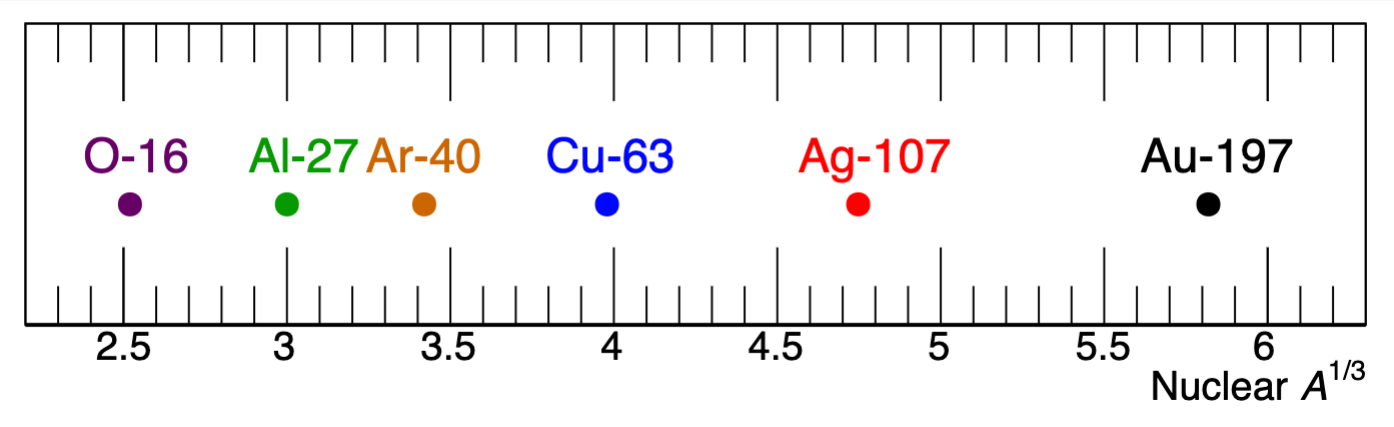
\includegraphics[width=0.85\linewidth]{figs/figure_A.png}
    \caption{Caption}
    \label{fig:figA}
\end{figure}

\begin{figure}
    \centering
    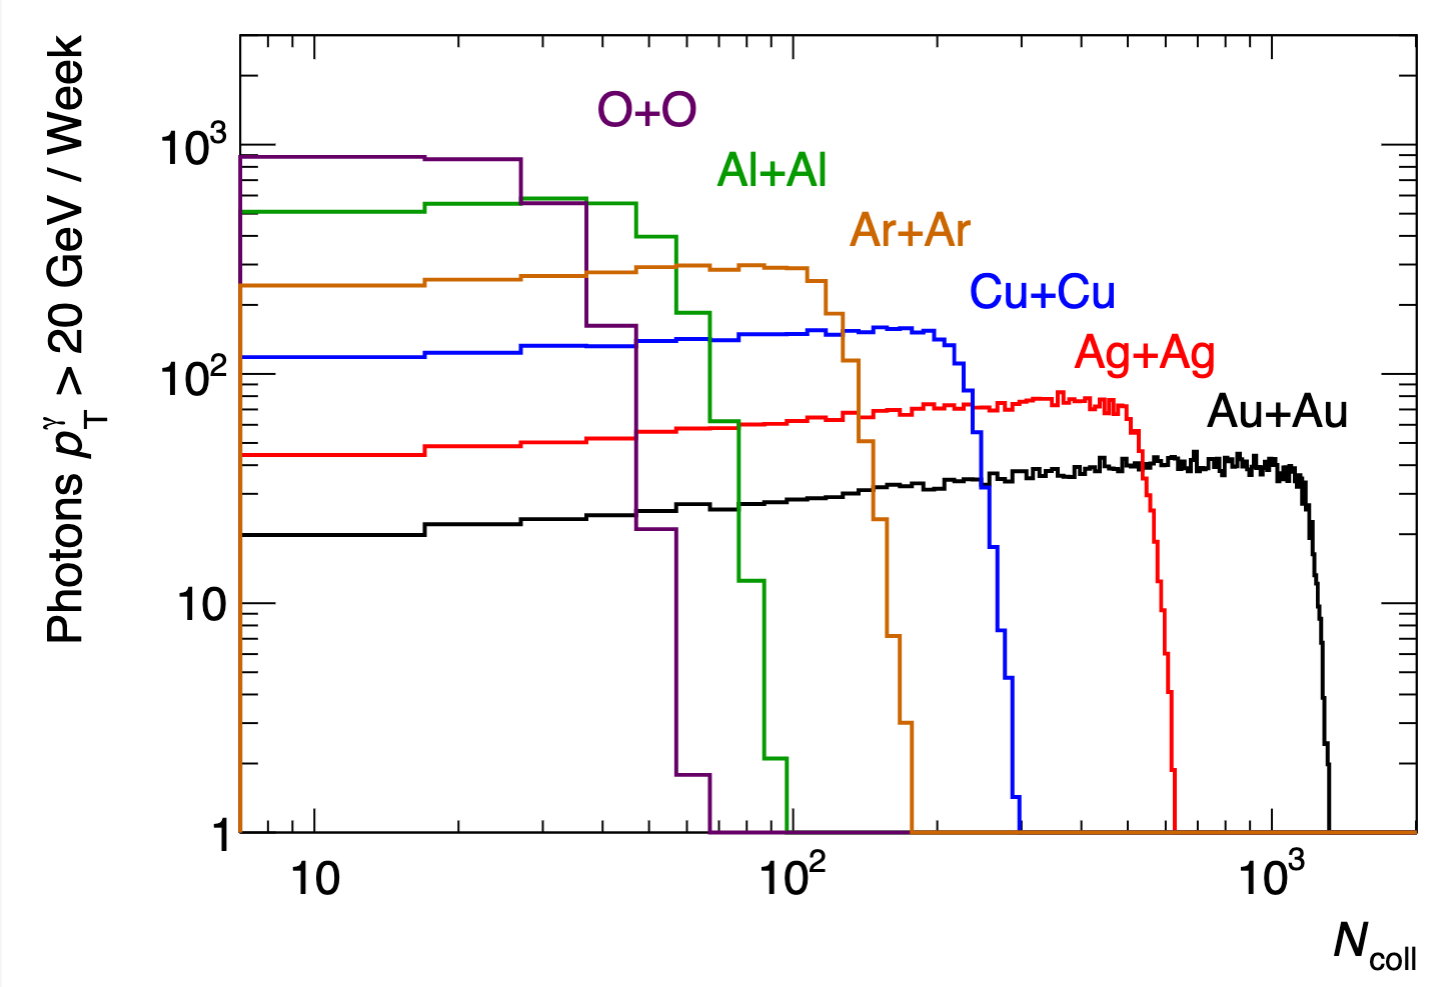
\includegraphics[width=0.85\linewidth]{figs/figure_small_perweek.png}
    \caption{Caption}
    \label{fig:figSmallPhoton}
\end{figure}


%%%%%%%%%%%%%%%%%%%%%%%%%%%%%%%%%%%%%%%%%%%%%%%%%%%%%%%%%%%%%%%%%%%%%%%%%%%%%
\newpage
\section{Cryo-Week Details}
\label{sec:cryo20262027}

In Table~\ref{tab:cryoplan2026} and Table~\ref{tab:cryoplan2027} we detail the 28 cryo-weeks of potential running in 2026 and 2027 respectively.

\begin{table}
\centering
\begin{tabular}{ | c | l | }
\hline
Weeks & Designation \\ \hline
0.5  & Cool Down from 50 K to 4 K \\ \hline
2.0  & Set-up mode 1 (p$^{\uparrow}$p$^{\uparrow}$ at 200 GeV) \\ \hline
0.5  & Ramp-up mode 1 (8 h/night for experiment) \\ \hline
15.5 & Data taking mode 1 (p$^{\uparrow}$p$^{\uparrow}$ Physics) \\ \hline
2.0  & Set-up mode 2 (O+O at 200 GeV) \\ \hline
0.5  & Ramp-up mode 2 (8 h/night for experiment) \\ \hline
2.0 & Data taking mode 2 (O+O Physics) \\ \hline
2.0  & Set-up mode 3 (Ar+Ar at 200 GeV) \\ \hline
0.5  & Ramp-up mode 3 (8 h/night for experiment) \\ \hline
2.0 & Data taking mode 3 (Ar+Ar Physics) \\ \hline
0.5  & Controlled refrigeration turn-off \\ \hline \hline \hline
28.0 & Total cryo-weeks \\
\hline
\end{tabular}
\caption{Year 2026 run plan for 28 cryo-weeks with p$^{\uparrow}$p$^{\uparrow}$, O+O, and Ar+Ar 200~GeV collisions.\label{tab:cryoplan2026}}
\end{table}


\begin{table}
\centering
\begin{tabular}{ | c | l | }
\hline
Weeks & Designation \\ \hline
0.5  & Cool Down from 50 K to 4 K \\ \hline
2.0  & Set-up mode 1 (Au+Au at 200 GeV) \\ \hline
0.5  & Ramp-up mode 1 (8 h/night for experiments) \\ \hline
24.5 & Data taking mode 1 (Physics) \\ \hline
0.5  & Controlled refrigeration turn-off \\ \hline \hline \hline
28.0 & Total cryo-weeks \\
\hline
\end{tabular}
\caption{Year 2027 run plan for 28 cryo-weeks with Au+Au 200~GeV collisions.
\label{tab:cryoplan2027}}
\end{table}
\chapter{Summary}
\label{chap:summary}

sPHENIX will be the first new collider detector at RHIC in over twenty
years,  performing very high statistics studies of jet
production, jet substructure and open and hidden heavy flavor over an
unprecedented kinematic range at RHIC.  The experiment
is a specific priority of the DOE/NSF NSAC Long Range Plan and 
will play a critical role in the completion of the RHIC science mission by enabling qualitatively
new measurements of the microscopic nature of quark-gluon plasma.
sPHENIX is distinguihed by high rate capability and large acceptance, 
combined with high precision tracking and electromagnetic and hadronic calorimetry.

The effort to construct the experiment is officially underway, with
the DOE MIE project having been granted PD-2/3 approval in September
2019. First year of data taking will be 2023; the final year of sPHENIX operations in
2025 is dictated by BNL's reference schedule for the EIC project.

Each run in this three year period plays a critical role in fulfilling the 
sPHENIX science mission outlined in the NP Long Range Plan:
\begin{itemize}
\item Year-1 serves to commission all detector subsystems and full
  detector operations, and to validate the calibration and
  reconstruction operations essential to delivering the sPHENIX
  science in a timely manner.  Year-1 will
  also allow collection of a \auau data set enabling sPHENIX to repeat
  and extend measurements of ``standard candles'' at RHIC.
\item Year-2 will see commissioning of the detector for \pp collisions
 and collection of a large \pp reference data set, as well as a large \pAu data set
  for studies of cold QCD.
\item Year-3 is focused on collection of a very large statistics \auau
 data set for measurements of jets and heavy flavor observables with
  unprecedented statistical precision and accuracy.
\end{itemize}

The collaboration also sees a strong physics case for additional running in Year-4 to Year-5 (2026 - 2027), should the occasion
arise. This represents unique opportunities for collecting massive,
archival \apa and spin polarized \pp data sets in the final years of
RHIC operation. 



\cleardoublepage

\appendix
\chapter{Beam Use Proposal Charge}
\label{chap:charge}

The charge from the Associate Laboratory Director Berndt Muller was received by the sPHENIX Spokespersons on July 11, 2020.   The charge is included below.

\begin{verbatim}
For the Sept 10-11 meeting of the PAC I would like you to prepare the 
following documents and presentations:

STAR: Beam Use Request for Run-21 and Run-22

STAR and sPHENIX: Beam Use Requests for Runs 23-25

The BURs should be based on the following number of expected cryo-weeks:

2021:  24 (28)
2022:  20
2023:  24 (28)
2024:  24 (28)
2025:  24 (28)

Presentations only:

STAR: Update on spin physics and isobar run analyses
PHENIX: Update on ongoing analysis efforts and data archiving effort
sPHENIX: Update on EIC EoI based on sPHENIX

The Beam Use requests should be submitted in written form no later than 
August 31. 2020.
\end{verbatim}

\cleardoublepage

\backmatter

%\cleardoublepage
%\phantomsection
%\addcontentsline{toc}{chapter}{List of Tables}
%\listoftables

%\cleardoublepage
%\phantomsection
%\addcontentsline{toc}{chapter}{List of Figures}
%\listoffigures

\cleardoublepage
\phantomsection
\addcontentsline{toc}{chapter}{References}

\bibliographystyle{unsrturl}
\bibliography{refs}

\end{document}  %%%%%%%%%%%%%%%%%%%%%%%%%%%%%%%%%% End Document


